\documentclass[a4paper, oneside]{thesis}

\usepackage[utf8]{inputenc}
\usepackage[T1]{fontenc}
\usepackage{float}
\usepackage{pdfpages}

%%%%%%%%%%%%%%%%%%%%%%%%%%%%%%%%%%%%%%%%%%%%%%%%%%%%%%%%%%%%%%%%%%%%%%%%%%%%%%%%%%%%%%%%%%%%%%%%%
% DOCUMENT METADATA

\thesistype{Master's Thesis} % Master's Thesis, Bachelor's Thesis, Semester Thesis, Group Project
\title{Probing Language Models With Topic Models}

% Analyzing Language Models with Topic Models
% What Topics tell us about Language Models
% Topic Models, the key to understanding Bias in Language Models?
% The meaning of Topics in a Language Model
  
% Topic Models, the key to understanding Language Models?
% What Topic Models have to say about Language Models
% Topic Models and their opinion about Language Models
% Topic Models, an Insight into Language Models
% What Topics say about a Language Model
% What the Topics of a Language Model reveal
% What Topics of a Language Model reveal
% Language Models and the meaning of their Topics
% Looking deep into Language Models with a Topic Model Analysis
% Topic Models analyze Language Models
% A Topic-Analysis of Language Models (TALM)
% Topics and their insight into Language Models


\author{Franz Knobel}
\email{knobelf@student.ethz.ch}

\institute{Rycolab\\[2pt]
Computational Linguistics, Natural Language Processing and Machine Learning\\[2pt]
ETH Zürich}

% Optionally, you can put in your own logo here
%\logo{\includegraphics[width=0.2\columnwidth]{figures/disco_logo_faded}}

\supervisors{Clara Meister\\[2pt] Prof.\ Dr.\ Ryan Cotterell}

% Optionally, keywords and categories of the work can be shown (on the Abstract page)
%\keywords{Keywords go here.}
%\categories{ACM categories go here.}

\date{\today}

%%%%%%%%%%%%%%%%%%%%%%%%%%%%%%%%%%%%%%%%%%%%%%%%%%%%%%%%%%%%%%%%%%%%%%%%%%%%%%%%%%%%%%%%%%%%%%%%%

\begin{document}

\frontmatter % do not remove this line
\maketitle

\cleardoublepage

\begin{acknowledgements}
First and foremost, I would like to thank my supervisor Clara Meister. Her constant support in the form of motivation, feedback, fresh ideas and explanations was an invaluable help and I appreciated it greatly. 
Secondly, I would like to thank Denise Spicher from the study administration. Her persistent moral and administrative support throughout my studies made ETH feel like home. 
I would also like to thank my supervising professor Ryan Cotterell for his valuable insights into my work. 
Furthermore, the continuous support from friends and family helped me stay on track over those six months. Thank you all for being there for me!
\end{acknowledgements}


\begin{abstract}
This thesis introduces a new approach to analyzing language models with topic models. Specifically, we generate corpora from language models and then use topic models to analyze the language models via these corpora. This analysis reveals which areas of the semantic space language models used today are learning. We then compare the topic model distributions of the model-generated corpora with a topic model fitted to its training data---using a metric based on the Jensen-Shannon distance---to assess whether the innate topic distribution of a language model is a reflection of its training or a byproduct of its inductive biases. Through the variation of several factors, e.g. model architecture and generation strategy, we are able to gain a better understanding of the inductive biases of certain components that are part of the language modeling pipeline. 
\end{abstract}

\tableofcontents

\mainmatter % do not remove this line

% Start writing here
\chapter{Introduction}

Pretrained language models have yielded state-of-the-art performance on a myriad of tasks along with reducing the computational resources often required to train NLP models by providing an advanced starting point for practitioners. Yet, due to the sheer size of the support of these models, the learned probability distribution over natural language strings is difficult to analyze. The support of the distribution alone---the set of all possible strings that can be built using a specific vocabulary---is countably infinite. While a number of techniques have recently been proposed for analyzing the attributes of natural language that these models learn \cite{desintpro, alain2016understanding, pandit2021probing, koto2021discourse, belinkov2022probing}, it is still unclear what portions of the semantic space they learn (or fail) to represent.

One set of techniques used to find out more about the specific properties of language learned by these models is called probing. Probing is a method where supervised models are trained to predict linguistic properties from text. If a property is encoded in the text, the resulting accuracy of the aforementioned models is assumed to be high. Probing is applied relative to some baseline and we just \textit{assume} the probe found the property. This process raises the question whether the probe interpreted the text it was given or just learned the task itself. \cite{desintpro}

We propose an alternative method to probing language models by utilizing a known technique from natural language processing: the topic model. Topic models cluster documents from a corpus into topics and provide insight into what words occur together and how often they occur in the analyzed text, i.e. the semantic space. Language models are generally trained on vast and unstructured text corpora. Through this they learn key mechanics of natural language \cite{rytting2021leveraging}, s.t. they can be fine-tuned on a variety of NLP tasks. This requires the model to learn the hidden structures and connections between sentences and words in the training corpus. That way, the model will be able to apply the learned knowledge to different subtasks, e.g. prediction of news articles or movie reviews. We call that generalizing beyond the training data. The problem with generalizing is that we hardly know how to control what the language model generalizes and what not, apart from the training data \cite{MarasovicGradient2018NLP}. 

By analyzing the semantic space with topic models, we try to gain a better understanding of the language model and the assumptions it makes to generalize beyond the observed data, i.e. the inductive bias. The inductive bias is encoded in the language modeling algorithm and therefore difficult to analyze from these \textit{black boxes}. By sampling strings (also called documents) from a pretrained language model, we generate a corpus. This corpus should provide an unbiased representation of the information learned by the model. We then train topic models---using techniques such as Latent Dirichlet Allocation (LDA) \cite{blei2003latent}---to understand the distribution over topics that the language model captures. Finally, we compare those distributions across different corpora to better comprehend this inductive bias.

We assume that a language model learns the language and therefore the semantic space of the learning data. By comparing the topic distributions from learned data to data generated by the trained language model, we might discover discrepancies in the comparison metric. Those discrepancies ought to indicate that the prior assumption, meaning the inductive bias, skews the models topic distribution. For example, this could hint towards the fact that models favor learning generalizations over specific semantic spaces. By comparing different topic models \cite{blei2003latent, neuralLDA} on different language models \cite{gpt-2, transformer-xl}, we expect the resulting topic models to provide us with valuable information about the impact the inductive bias of our language models has on future predictions.

In this thesis, we employ a combination of techniques from \textit{Topic Modeling} and \textit{Pretrained Language Models}. The first part of this thesis consists of creating a baseline. We train a Language Model (GPT-2 \cite{gpt-2}) and compare the learned topic model to the topic model learned from the original dataset. We then evaluate and compare topic models from different text corpora with each other using our own designed metric. The second part of this thesis focuses on analyzing the topic probability distributions to get further insights into where the found discrepancies in our metric originated from, i.e.:
\begin{itemize}
    \item the language model architecture,
    \item the sampling technique for generating text from a language model or
    \item design choices of the topic model (e.g. tokenization, model architecture, etc.).
\end{itemize}
To this end, we additionally train a second language model (Transformer-XL \cite{transformer-xl}) and expand our topic model technique with the neural LDA \cite{neuralLDA}. Moreover, we compare the impact of different sampling techniques for language models (Top-P sampling \cite{holtzman2019curious} vs. Typical sampling \cite{meister2022typical}) and various topic sizes ($\{2, 3, 5, 10, 20, 50, 100\}$). We also study the influence of the dictionary, i.e. the set of unique words, that our topic model uses for learning the topic distributions. By adding bigrams and trigrams to the dictionary, we hope to provide the topic model with more information about related words such that it can learn the semantic space better. 

This work exploits the abilities of topic models by applying them to a task for which they have not yet been used. By means of a topic analysis, we gain a better understanding of the characteristics of language learned by today's language models, i.e. the inductive bias. A deeper understanding opens the way to new research, for example in the direction of language model architecture, the way they are trained and employed for various NLP tasks, and the application of topic models.

\chapter{Background}
This chapter reviews the theories necessary for the main part of the thesis. As we are creating topic models of pretrained language models, we need to know what those are and how they work. In the following sections, we explore their relevant origin  on top of providing an overview on current evaluation and comparison techniques.

% =============================
\section{Language Modeling}
% =============================
\subsection{Definition and Application}
Language models are created to distill valuable insights from raw text without the help of a human. To name a few tasks of language models:
\begin{itemize}
    \item \textbf{Natural-language generation (NLG)} extracts and transforms information in the form of raw data or text into readable and human understandable text. 
    \item \textbf{Natural-language understanding (NLU)} takes text as input and translates it into a more formal representation, so that computer applications can understand it. For example simple commands given to robots or more complex ones, like comprehension of newspaper articles.
    \item \textbf{Automatic summarization of texts} produces a readable summary of a fragment of text and can be extractive or abstractive. Extractive summarization concatenates strings with different length without knowing what they actually mean. On the other hand, abstractive summarization creates a context sensitive summary by using a combination of statistical and linguistic properties of the analyzed text. \cite{gupta2010survey}
    \item \textbf{Machine translation} translates text or speech from one language to another.
    \item \textbf{Question answering}, with or without context, answers text questions from humans. Answers are created with knowledge from large databases. This is usually a knowledge database or an unstructured collection of natural language documents. The questions themselves can be closed or open-ended.
    \item \textbf{Speech recognition} creates text equivalent to any input in the form of audio speech. 
    \item \textbf{Optical character recognition (OCR)} scans visual input and transforms it into machine-encoded text. Such input can be to images of typed, handwritten or printed text in the from a scanned document, a photo of a document or a scene-photo.
    \item \textbf{Paraphrasing} is a subcategory of text-to-text generation and is the art of paraphrasing words, sentences and full texts.
\end{itemize}

The standard definition of a language model is a model of the probability distribution over strings $p(\mathbf{y})$ in a natural language. This model should provide an estimate of the (unconditional) probability of observing some string $\mathbf{y} \in\mathcal{Y}$, where $\mathcal{Y}$ is the set of all valid strings in a language. Different attempts over time resulted in different model architectures, e.g. the n-gram (unigram, bigram, trigram, etc.) model, the log-linear model and the neural model. For large pretrained language models, neural language models deliver state of the art results on various NLP tasks. Compared to traditional language models, neural models allow conditioning on increasingly larger contexts with only linear increases in the number of parameters. They parameterize words as vectors (word embeddings) and use these vectors as inputs. These parameters are learned as part of the training process of neural models. Each neural model has a specifically designed architecture for the data it was designed to learn, which puts restrictions on the learning algorithm. Furthermore, the ability to generalize to unseen data introduces an inductive bias to our model, which in itself is not a bad thing. In fact, we need our model to generalize to unseen data. This way, the model will be able to apply the learned knowledge to different subtasks it was not trained for, e.g. prediction of news articles or movie reviews.

A first attempt to neural language modeling by Bengio et al., 2003 \cite{bengio2003neural} uses feed-forward neural network models. However, with increasing lexicon size, the computations regarding the output layer become computationally intractable. The reason being that the predicted output on a particular input needs to be a probability distribution over the entire lexicon (softmax over the vocabulary). With recurrent neural networks (RNN), this limitation is avoided as they can learn arbitrary long influences without being dependant on the size of the lexicon (infinite context). In an RNN, each node is aware of its direct predecessor and the information from earlier nodes is only indirectly available through the encoding of the encodings. This leads to a loss of information as the lexicon gets bigger.

% =======================================
\subsection{Attention Mechanism}
The attention mechanism poses a solution to the loss of information in large RNN networks. It overcomes the limitation of the fixed-size vector representation of the input sequence. Attention comes in the form of a hidden layer and computes a categorical distribution (or hierarchy of categorical distributions) over the input. The input can be the direct words or intermediate input from other layers. \cite{kim2017structured}

The concept of the attention mechanism was introduced by Bahadanau et al., 2014 \cite{bahdanau2014neural} for machine translation (see fig. \ref{fig:attentionMT}) and has demonstrated success on various NLP tasks. 
\begin{figure}[H]
    \centering
    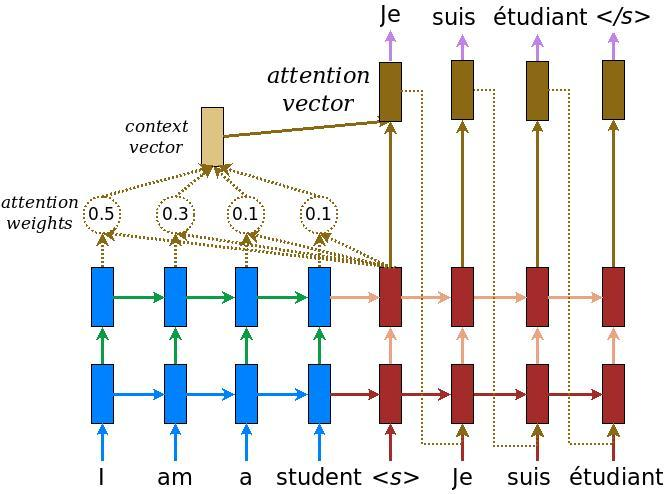
\includegraphics[width=0.7\textwidth]{figures/attention}
    \caption{Attention Mechanism for machine translation with encoder (blue) and decoder (red). \cite{attentionmechanism}}
    \label{fig:attentionMT}
\end{figure}
Later, Yang et al., 2016 \cite{yang2016hierarchical} introduced the intra or self-attention mechanism for document classification. Because not all words contribute equally to the representation of the meaning of a sentence, the attention mechanism was adapted to a word level, such that it relates different positions of a single sequence to compute a representation of the sequence. 

Vaswani et al., 2017 \cite{vaswani2017attention} exploited this technique in their proposed architecture, the Transformer, and introduced an adaptation of self-attention and the new multi-head attention. 

% =======================================
\subsubsection{Self-Attention}
The self-attention mechanism \cite{vaswani2017attention} makes inputs aware of each other and tells them which are the more important ones. The outputs of this mechanism are aggregates of these interactions and the attention scores. Every input is represented by three vectors, i.e. a key $k$, a query $q$ and a value $v$. They are a product of the input vector and three global weight matrices, i.e. $W^Q,\;W^K,\;W^V$ (see fig. \ref{fig:selfattention}), which are learned during the training process. Every input uses those matrices to calculate their three representations.
\begin{figure}[H]
    \centering
    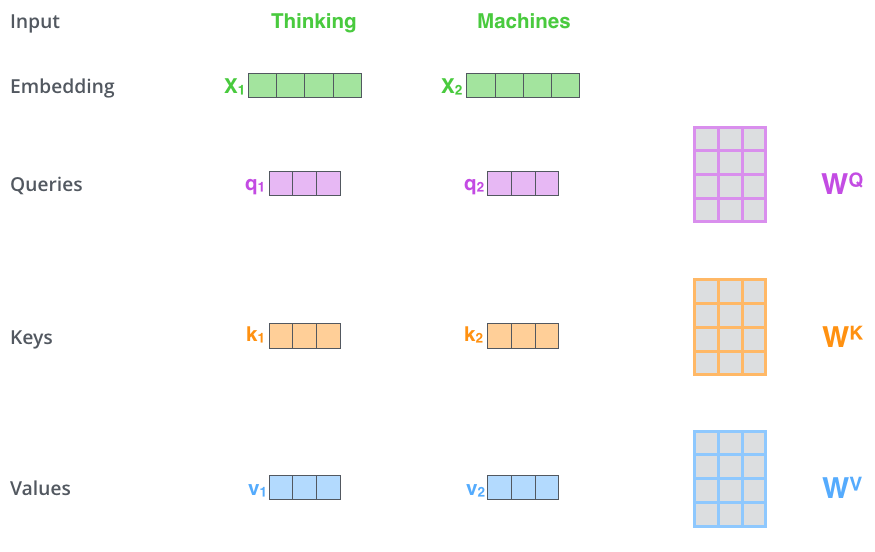
\includegraphics[width=0.7\textwidth]{figures/selfattention}
    \caption{Self-Attention Mechanism: Illustrating input/embeddings (green), query (pink), keys (orange) and values (blue). \cite{illustratedtransformer}}
    \label{fig:selfattention}
\end{figure}
Depending on where to put attention, different scoring functions are used. In the Transformer architecture, the scaled-dot-product (see fig. \ref{fig:scaled-dot-product-attention}) is used.
\begin{figure}[H]
    \centering
    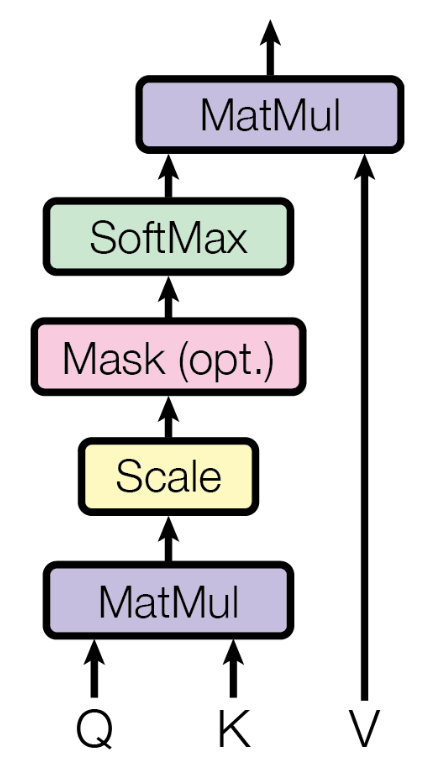
\includegraphics[width=0.2\textwidth]{figures/scaled-dot-product-attention}
    \caption{Scaled Dot-Product. \cite{vaswani2017attention}}
    \label{fig:scaled-dot-product-attention}
\end{figure}
The output of the scaled-dot-product attention are the weighted values $V$ according to eq. \ref{eq:sdp}. 
\begin{equation}\label{eq:sdp}
    \text{Attention}(\mathbf{Q},\mathbf{K},\mathbf{V})=\text{softmax}\left(\frac{\mathbf{Q}\mathbf{K}^T}{\sqrt{d_k}}\right)\mathbf{V}
\end{equation}

% =======================================
\subsubsection{(Masked) Multi-Head Attention}\label{sec:multheadat}
the goal is to make the different inputs aware of each other at different positions. Apart from the collectively learned weight matrices ($W^Q,\;W^K,\;W^V$), we calculate the output for input $x_1$ by using the query vector $q_1$ in all self-attentions instead of using each their own query vector ($q_2, q_3, ...)$. The resulting self-attention vectors are then summed up giving us the multi-head attention vector for input $x_1$. This process is repeated for every input, but in practice, this is done very efficiently with matrix multiplications (see fig. \ref{fig:multi-head-attention}).
\begin{figure}[H]
    \centering
    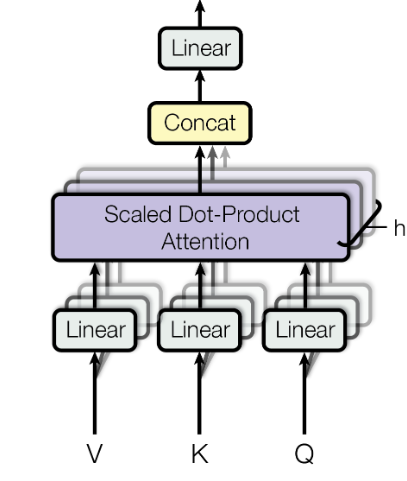
\includegraphics[width=0.3\textwidth]{figures/multi-head-attention}
    \caption{Multi-Head Attention. \cite{vaswani2017attention}}
    \label{fig:multi-head-attention}
\end{figure}

The masked multi-head attention is a slight variation of the normal multi-head attention. Before the softmax step (see fig. \ref{fig:scaled-dot-product-attention}), the multi-head-attention layer uses only earlier positions in the output sequence. This is done by setting all future positions to minus infinity. 

% =======================================
\subsection{The Transformer}
Vaswani et al., 2017 \cite{vaswani2017attention} posed a solution, to the limitations of the RNN architectures by combining original attempts to neural language modeling, which were based on feed-forward networks, with the attention mechanism. The so called Transformer architecture relies entirely on the attention mechanism to draw out the global dependencies between the input and output \cite{illuaatte}. It predicts $y_t$ by only using the $k$ most recent inputs, $x_{t-k+1},...,x_t$ (fig. \ref{fig:feedforward0}). To be able to depend on the most $k$ recent inputs, the model must assume a strong conditional independance.
\begin{figure}[H]
    \centering
    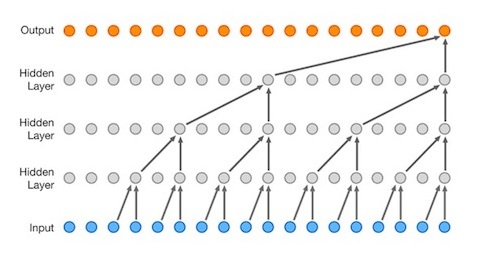
\includegraphics[width=0.9\textwidth]{figures/feedforward0}
    \caption{Illustration of an autoregressive feed-forward language model. \cite{feedforward}}
    \label{fig:feedforward0}
\end{figure}
Please note that in the next step the output is generated conditioned on the $k$ most recent inputs and becomes part of the input. The window of $k$ inputs then shifts one step to the right (fig. \ref{fig:feedforward1}).
\begin{figure}[H]
    \centering
    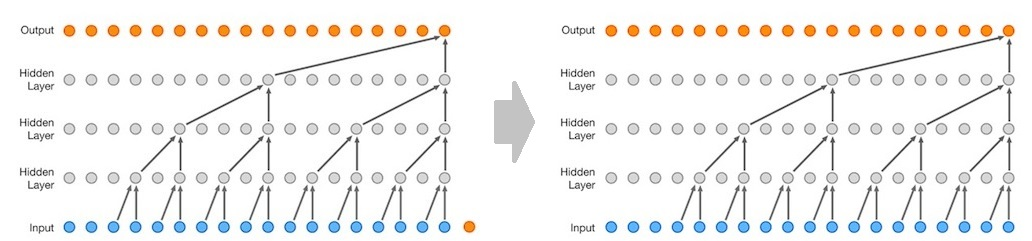
\includegraphics[width=1.0\textwidth]{figures/feedforward1}
    \caption{Illustration of the next step of an autoregressive feed-forward language model. \cite{feedforward}}
    \label{fig:feedforward1}
\end{figure}
The originally proposed Transformer architecture (see fig. \ref{fig:transformer-vis}) is an alteration of the sequence-to-sequence or encoder-decoder model \cite{attentionmechanism}. 
\begin{figure}[H]
    \centering
    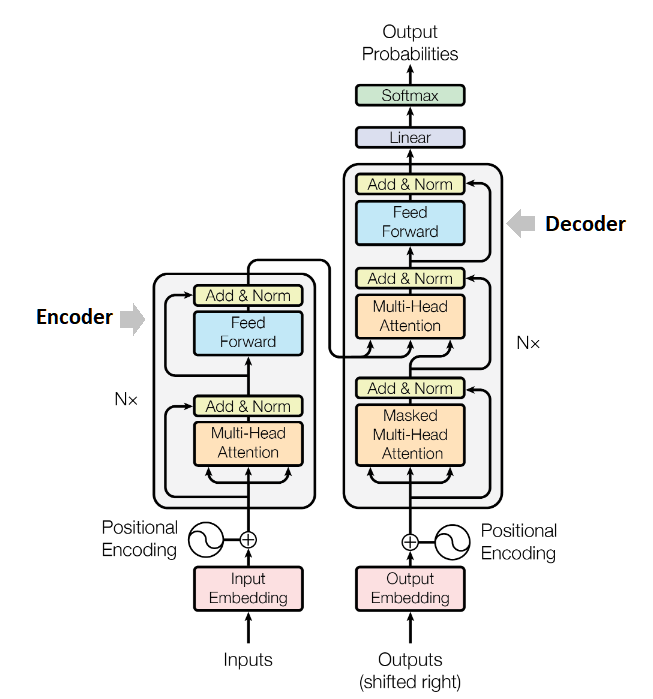
\includegraphics[width=0.7\textwidth]{figures/transformer}
    \caption{Illustration of the original Transformer Architecture. \cite{vaswani2017attention}}
    \label{fig:transformer-vis}
\end{figure}
Fig. \ref{fig:transformer-vis} just visualizes the incorporation of one encoder and one decoder. In practice, multiple encoders and decoders are put in series (see fig. \ref{fig:transformer-mult}).
\begin{figure}[H]
    \centering
    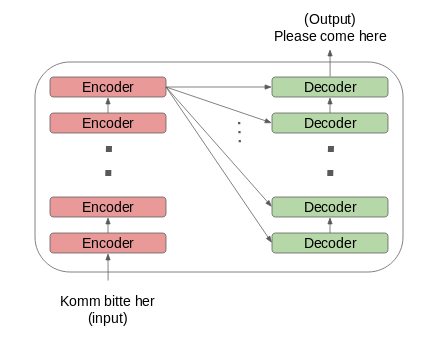
\includegraphics[width=0.6\textwidth]{figures/mult_trafo}
    \caption{Illustration of the encoder-decoder stack. \cite{howdotrafo}}
    \label{fig:transformer-mult}
\end{figure}
We can see that first the learned embeddings get encoded with a positional encoding. This is done by adding a one-hot vector to the embedding, which indicates the position of each word. 

The encoder encodes the full sequence into a context vector with fixed length. It is doing that by stepping through the input time steps. In the Transformer architecture this context vector comes in the form of a set of attention vectors $K$ and $V$. 

The decoder steps through the output time steps. While doing that, it reads from the two attention vectors, $K$ and $V$, mentioned before. These are used by each decoder in its \textit{Multi-Head Attention} (see sec. \ref{sec:multheadat}) block and help the decoder focus on appropriate places in the input sequence. After multiple decoding steps, the output after a linear and softmax block is a probability distribution where a word is sampled from (see sec. \ref{sec:gentext}). The sampled word of each iteration is then appended to the original input and again fed into the decoder to calculate the next output, and so on. Just like with the encoder inputs, the positional encodings are added to the word embeddings at every iteration. 

After basic training or pretraining, the language model is usually fine-tuned for specific NLP tasks. Fine-tuning means training on a task-specific dataset. Depending on performance and task, additional linear layers are added at the end of the language model and some parameters of the model are frozen, i.e. they do not change while fine-tuning. \cite{trafoarch}

% =======================================
\subsection{Transformer Based Architectures}
The realization that the encoder and decoder part can be used separately for different NLP tasks led to different language models based on the Transformer architecture. 

% =======================================
\subsubsection{GPT-1}
Focusing research on the decoder part (see fig. \ref{fig:gpt}) resulted in the well-known GPT-1 model \cite{radford2018improving}. GPT-1 computes the probability $p(\mathbf{y})$ of a complete sentence given nothing or a beginning of a sentence, where $\mathbf{y}\in\mathcal{Y}$ and $\mathcal{Y} = \{\textsc{bos}+\mathbf{v}+\textsc{eos}\mid \mathbf{v} \in \mathcal{V}^* \}$. $\mathbf{y}= \langle y_1, y_2, \dots\rangle$ is a sequence consisting of natural language tokens  $y\in\mathcal{V}$ from a set vocabulary $\mathcal{V}$, padded with special \textsc{bos} and \textsc{eos} tokens to demarcate the beginning and end of a string, respectively. 
\begin{figure}[H]
    \centering
    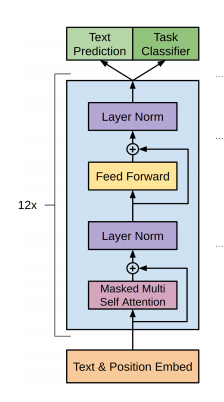
\includegraphics[width=0.3\textwidth]{figures/gptarch}
    \caption{The GPT-1 Architecture. \cite{radford2018improving}}
    \label{fig:gpt}
\end{figure}
GPT-1 is a unidirectional model, meaning it is only aware of what came before. It learns using unlabeled data and is fine-tuned by providing examples of specific downstream tasks like classification, sentiment analysis, textual entailment, etc. Its major advantage is the massive volume of data it was pretrained on. This makes adapting the \textit{raw}-trained model possible for different NLP tasks with very little data. 

% =======================================
\subsubsection{GPT-2}
The GPT-2 \cite{gpt-2} model pretty much follows the architecture of the original GPT-1 model (see fig. \ref{fig:gpt2}). New additions are that each sub-block now has the layer normalization from the end in the beginning and to the layer normalization block in the middle an additional layer is added (see fig. \ref{fig:gpt2}). The weights of the residual layers (used at initialization) are newly scaled by a factor of $1/\sqrt{N}$ where $N$ is the number of residual layers. This accounts for the accumulation on the residual path with model depth. The vocabulary is expanded to 50,257 tokens, the context size to 1024 tokens and the batchsize to 512 documents \cite{gpt-2}. This resulted in 1.5B parameters for the largest model in contrast to the 117M parameters for GPT-1. 
\begin{figure}[H]
    \centering
    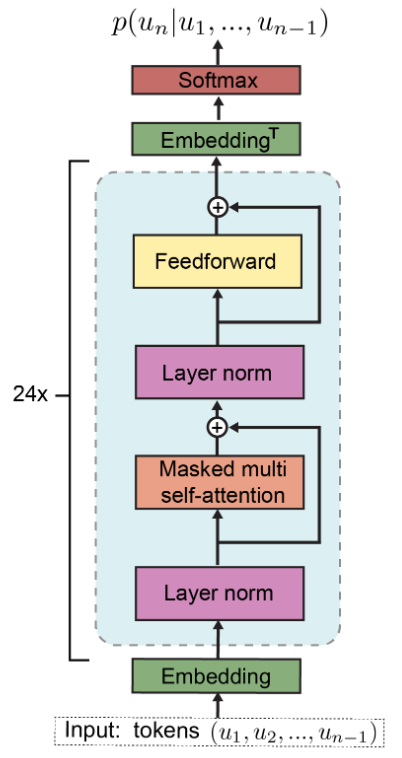
\includegraphics[width=0.4\textwidth]{figures/gpt2}
    \caption{The GPT-2 Architecture. \cite{heilbron2019tracking}}
    \label{fig:gpt2}
\end{figure}
The model was trained on the WebText dataset \cite{radford2019language}. This dataset was created by scraping web pages which have been curated, respectively filtered, by humans and then filtered with a combination of content extractors. Important to note is that Wikipedia was not included as it is a common data source for other datasets and could complicate analysis due to overlapping training data with test evaluation tasks. \cite{gpt-2}

% =======================================
\subsubsection{Transformer-XL}
Transformer-XL \cite{transformer-xl} builds upon the decoder part of the Transformer architecture. It extends the memory of the fixed-length context by conditioning on the sequences that came before. Without disrupting temporal coherence, Transformer-XL additionally solves the issue of context fragmentation. Context fragmentation is one of the main limitations of the original Transformer model and happens when a model tries to fit a document, the document gets segmented because it is too big, and long-term dependencies are then lost. 

The decoder from the original Transformer architecture is modified as such, that it functions like a cell from the RNN architecture where the memory transfer happens in the attention mechanism (see fig. \ref{fig:transformer-xl-arch}).
\begin{figure}[H]
    \centering
    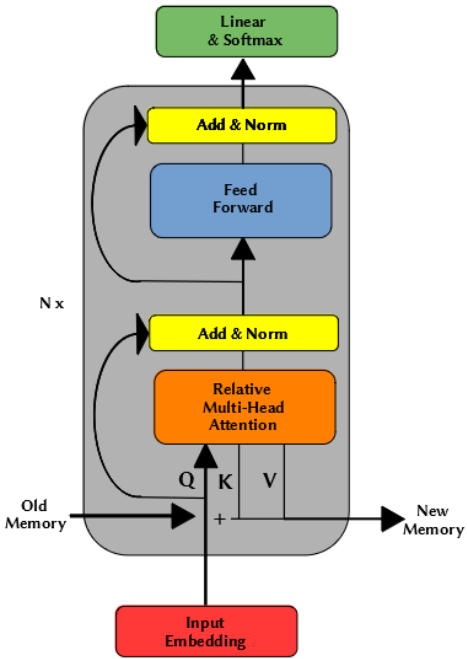
\includegraphics[width=0.5\textwidth]{figures/transformer-xl-arch}
    \caption{The Transformer-XL model. \cite{dowdell2020language}}
    \label{fig:transformer-xl-arch}
\end{figure}
Transformer-XL was trained separately on multiple datasets including Wikitext-103 and experiments have shown that it learns much longer dependencies.

% =======================================
\subsubsection{Probing Language Models}
A language model tries to learn the hidden structures and connections between sentences and words in the training corpus. To shed light on these hidden properties, researchers try to isolate linguistic phenomena through specifically designed multi-class classification problems, so called probing tasks. We assume that if a system has a good performance on a probing task, it has encoded the phenomena we were probing for. Those probes can have a low computational cost but there is a hidden complexity, i.e. we do not know the ideal setup. This means, we do not know how complex our probe has to be to find a property, e.g. whether a linear model suffices or deep learning is required. Thus, what part of the training data we use for training the probe, is rather unclear. We know in fact that with enough training data, a complex enough model is able to learn any linguistic phenomena we want it to find, and we therefore have to be aware of false positives. Recent studies have shown that it is definitely possible to memorize a good amount of specific labeling decisions without being dependant on the representation's linguistic properties. \cite{desintpro, gul2019linspector, hewitt2019structural, white2021non, lingwis}

% =======================================
\section{Generating Text From Pretrained Models}\label{sec:gentext}
% =======================================
\subsection{Ancestral Sampling}\label{sec:sampling}
Based on the standard definition of a language model and therefore on an autoregressive language model $p_\theta$, a string $\mathbf{y}\sim p_\theta$ can be generated from the conditional probability distributions. Given the relationship in eq. \ref{eq:joint}, we can set $y_1 = \textsc{bos}$ or the empty string, and sample $y_t\sim p(\cdot\mid\mathbf{y}_{<t})$ until we sample the \textsc{eos} token. 
\begin{equation}\label{eq:joint}
    p(\mathbf{y})=p(y_1,...,y_t)=p(y_1)\cdot p(y_2\mid y_1)\cdot...\cdot p(y_t\mid y_{t-1})=\prod_{t=1}^{|\mathbf{y}|} p(y_t\mid\mathbf{y}_{<t})
\end{equation}
This means, using the chain rule of probability, we can model the probability of an entire string as the product of the conditional probability of each word given its prior context. Here we define $\mathbf{y}_{<t} = \langle y_1, \dots, y_{t-1}\rangle$. We call this ancestral sampling, as we start by sampling the ancestor $p(y_1)$, then $p(y_2\mid y_1)$ and so on.

% =======================================
\subsection{Top-P Sampling}
In Top-P or \textit{nucleus} sampling \cite{holtzman2019curious} we choose from the smallest possible set of words whose cumulative probability exceeds the probability $p$. Among this set of words, the probability mass is redistributed. Thus, the number of words in the set can dynamically increase and decrease according to the probability distribution of the next word.

Formally, Top-P sampling reduces the set of words $\mathcal{V}$ from the distribution $p(y\mid y_{1:i-1})$ to the smallest subset $\mathcal{V}^{(p)}\subset \mathcal{V}$, s.t.
\begin{equation}
    \sum_{y\in \mathcal{V}^{(p)}}{p(y\mid y_{1:i-2})}\geq p.
\end{equation}
Illustrated by an example in fig. \ref{fig:topp}, we set $p=0.93$. Top-P sampling chooses the minimum number of words, such that their summed up probability mass exceeds $p=93\%$. Here, this set is defined as $\mathcal{V}_{top-p}$ (per definition, equal to $\mathcal{V}^{(0.93)}$). On the left side the 9 most likely words have to be included, where on the right side only the top 3 words are needed to exceed $93\%$. \cite{trafogen}
\begin{figure}[H]
    \centering
    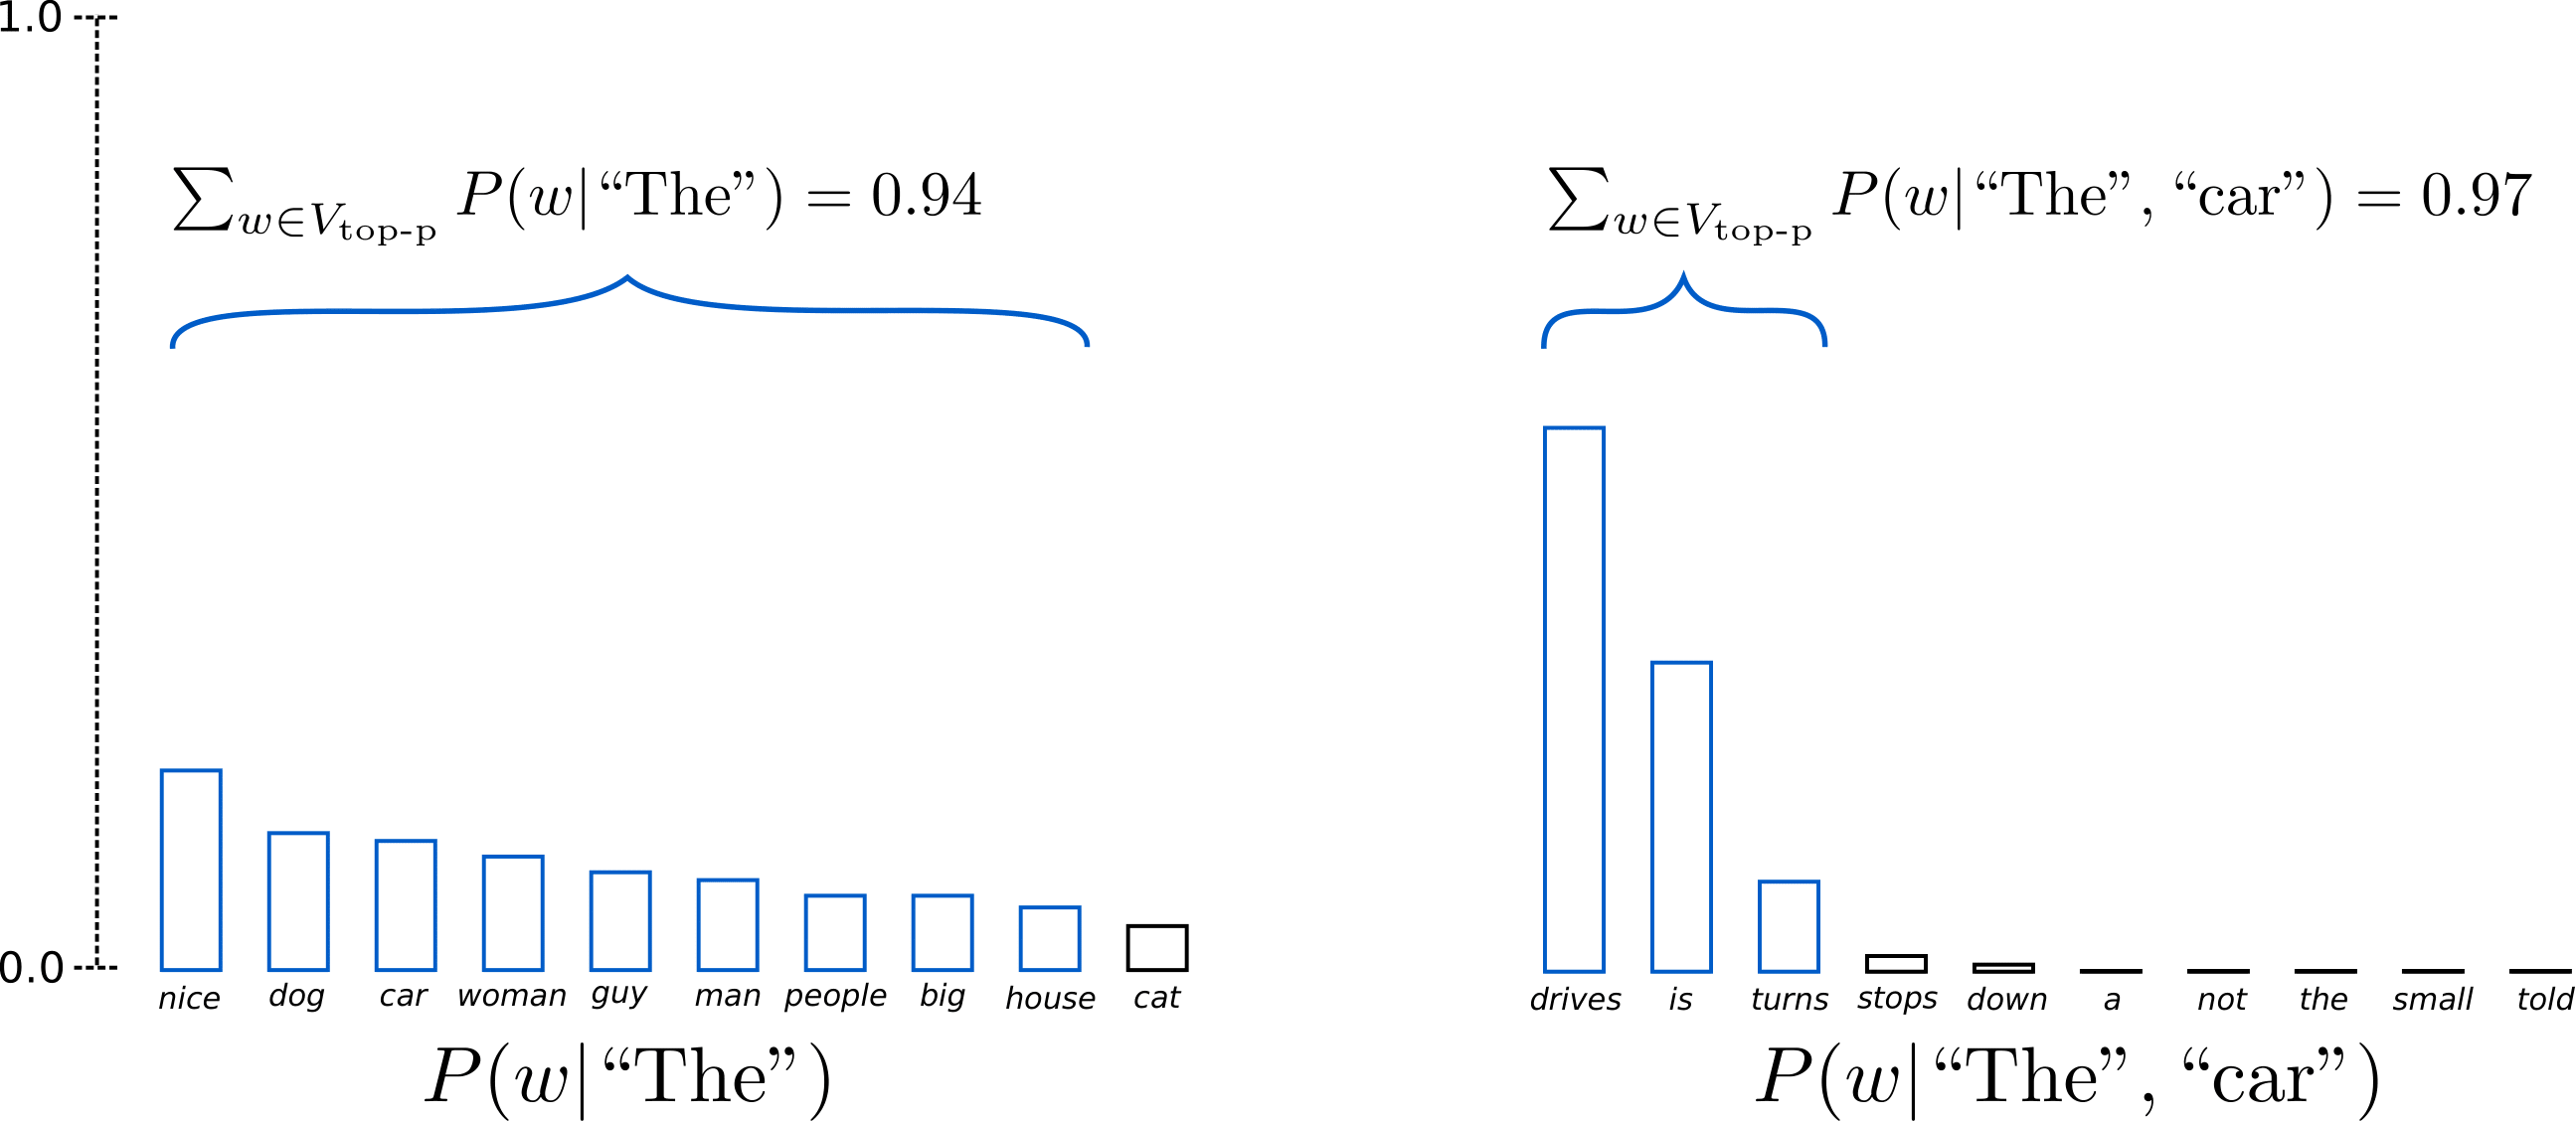
\includegraphics[width=1.0\textwidth]{figures/topp}
    \caption{Top-P sampling example. \cite{trafogen}}
    \label{fig:topp}
\end{figure}

% =======================================
\subsection{Typical Sampling}
Typical sampling \cite{meister2022typical} tries to imitate human communication. Instead of choosing words that have a certain probability mass, like Top-P sampling, it samples according to the information content of the words. The information content of the set of words is expected to be close to the information content of the model. Which is equal to its conditional entropy, i.e. we assume that for human-like text eq. \ref{eq:toppdiff} is very small.
\begin{equation}
    \varepsilon=\left|H(p(\cdot\mid \mathbf{y}_{<t}))+log\, p(y_t\mid \mathbf{y}_{<t})\right|
\label{eq:toppdiff}
\end{equation}
The sampled distribution is then limited to the word subset as $\mathcal{V}^{(\tau)}\subseteq\mathcal{V}$. This subset has to minimize eq. \ref{eq:toppdiff2} at each time step. Therefore, the subset changes constantly. 
\begin{equation}
    \sum_{y\in\mathcal{V}^{(\tau)}}{\varepsilon},\text{ s.t. }\sum_{y\in\mathcal{V}^{(\tau)}}{p(y\mid \mathbf{y}_{<t})}\geq\tau.
\label{eq:toppdiff2}
\end{equation}
After reducing the word count in the subset, it has to be renormalized according to eq. \ref{eq:norm}.
\begin{equation}
    \begin{aligned}
        \pi(y\mid\mathbf{y}_{<t})=\left\{
        \begin{matrix*}[l]
            p(y\mid\mathbf{y}_{<t})/\sum_{y\in\mathcal{V}^{(\tau)}}{p(y\mid\mathbf{y}_{<t})}, & \text{if }y\in \mathcal{V}^{(k)} \\ 
            0, & \text{else}
        \end{matrix*}\right.
    \end{aligned}
\label{eq:norm}
\end{equation}

% =======================================
\subsection{Evaluation and Metrics}
In general, it is a good idea not only to evaluate our trained model by the loss or the accuracy, but also by testing them on an actual task. We call that extrinsic evaluation. By embedding our trained model directly in an application and measuring how much the application improves, we can immediately see how different models perform and behave. For example, if we want to measure the difference in performance of two models trained for speech recognition. To achieve that, we run the speech recognizer two times and can then directly see which one of the results is a more accurate transcription. This process requires us to train a full system, which makes it computationally expensive and, depending on your model and processing power, very slow. Therefore, it is sometimes more practical to have a metric (better than accuracy or loss) that can cost-efficiently evaluate potential improvements in a language model and its quality, independent of any application. We call this intrinsic evaluation. This evaluation needs, apart from the model, a test set. The models we want to compare are then fitted onto this test set and whichever model assigns a higher probability, or rather more accurately predicts the test set, is a better model. The metric itself is based on the probability of the test set. Important is that any part of the test set should not be used for training. Otherwise, it would introduce a bias to the model which makes the probabilities for the test set higher than they actually are. An example for a widely used probability-based metric is Perplexity, or short PP. \cite{slp3}

% =======================================
\subsubsection{Perplexity}\label{sec:perplexity}
Perplexity \cite{perplexity} is an intrinsic evaluation method and is the inverse probability of the test set, normalized by the number of words. For a test set$_w=w_1,w_2,...,w_N$ the Perplexity is:
\begin{equation}
    PP(W)=\sqrt[n]{\frac{1}{P(w_1,...,w_N)}}.
    \label{eq:perplexity}
\end{equation}
To a human-like and syntactically correct text, a model assigns a high probability. Low probabilities should be the result of fake, incorrect, or highly infrequent sentences. Therefore, the best model is going to be the one that assigns the highest probability to a real and correct test set. By assigning a high probability, the model is not perplexed (surprised) by it (see fig. \ref{fig:perplexity}). This implicates that a language model with low perplexity has a good understanding of how the language works. A simpler interpretation of the perplexity score is interpreting it as the weighted branching factor. This means, if we have a perplexity of 42, the model is confused because it has to pick from 42 words when trying to guess the next word. \cite{perplexity}
\begin{figure}[H]
    \centering
    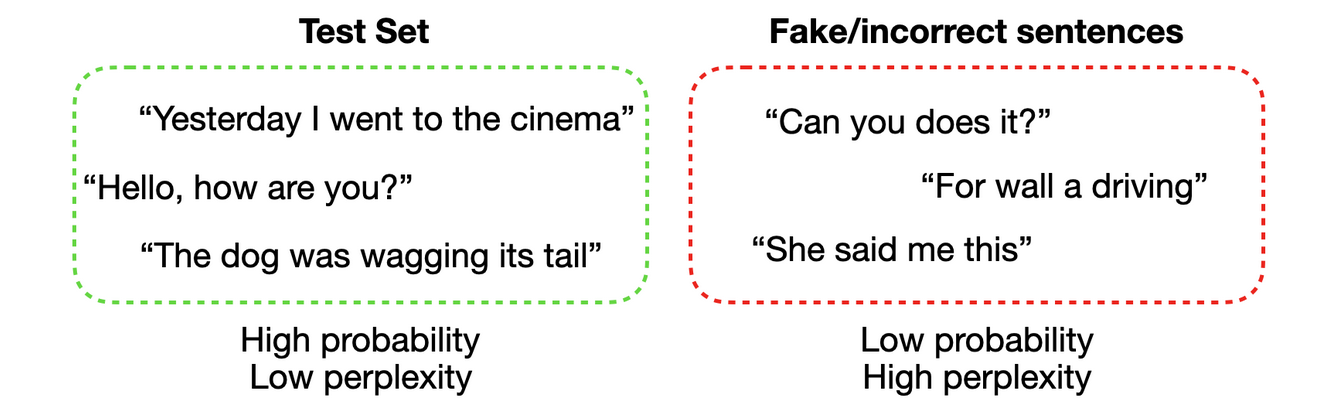
\includegraphics[width=1.0\textwidth]{figures/perplexity_example}
    \caption{Example of the Perplexity score. \cite{perplexity}}
    \label{fig:perplexity}
\end{figure}
Perplexity can also be defined as the exponential of the cross-entropy (see eq. \ref{eq:crosspp}), which is equivalent to the previous definition (eq. \ref{eq:perplexity}).
\begin{equation}
    PP(W)=2^{H(W)}=2^{-\frac{1}{N}log_2 P(w_1,...,w_N)}
\label{eq:crosspp}
\end{equation}

% =======================================
\section{Topic Modeling}
% =======================================
\subsection{Definition and Application}
A \textit{topic} is normally a phrase or a set of words that describes the content of a text. Topic modeling tries to find such topics. It is an unsupervised machine learning technique which has the ability to analyze a set of documents. Within those documents it detects patterns in multiple sentences down to the word level. It then clusters groups of words and similar expressions to best characterize this set of documents. This technique is useful for a wide range of data analysis from social media posts, emails, chats, customer support conversations, up to cancers' genomic samples. The process of dividing a corpus can in general be divided into two parts:
\begin{enumerate}
    \item A set of topics, where the topic is described in some specific way
    \item Multiple sets of grouped documents according to the topics they cover
\end{enumerate}
We assume that every document is represented by a distribution over topics. This distribution is the result of the probability mass for every topic covering this document. Those topics are defined and learned in the process, like latent variables. It is an unsupervised technique and does not require a training dataset. Hidden patterns and insights are found in the process. This does not guarantee accurate results. \cite{tmint} 

An well-known topic modeling technique is called latent Dirichlet allocation (LDA) \cite{blei2003latent}. 

% =======================================
\subsection{Latent Dirichlet Allocation (LDA)}
LDA \cite{blei2003latent} is a statistical model of a collection of documents. The model assumes that a document consists of multiple topics and a topic of multiple words. This variability of random multinomial distributions is modeled with the help of the Dirichlet distribution. The Dirichlet distribution basically models a probability distribution of probability distributions. The figure below illustrates the intuition:
\begin{figure}[H]
    \centering
    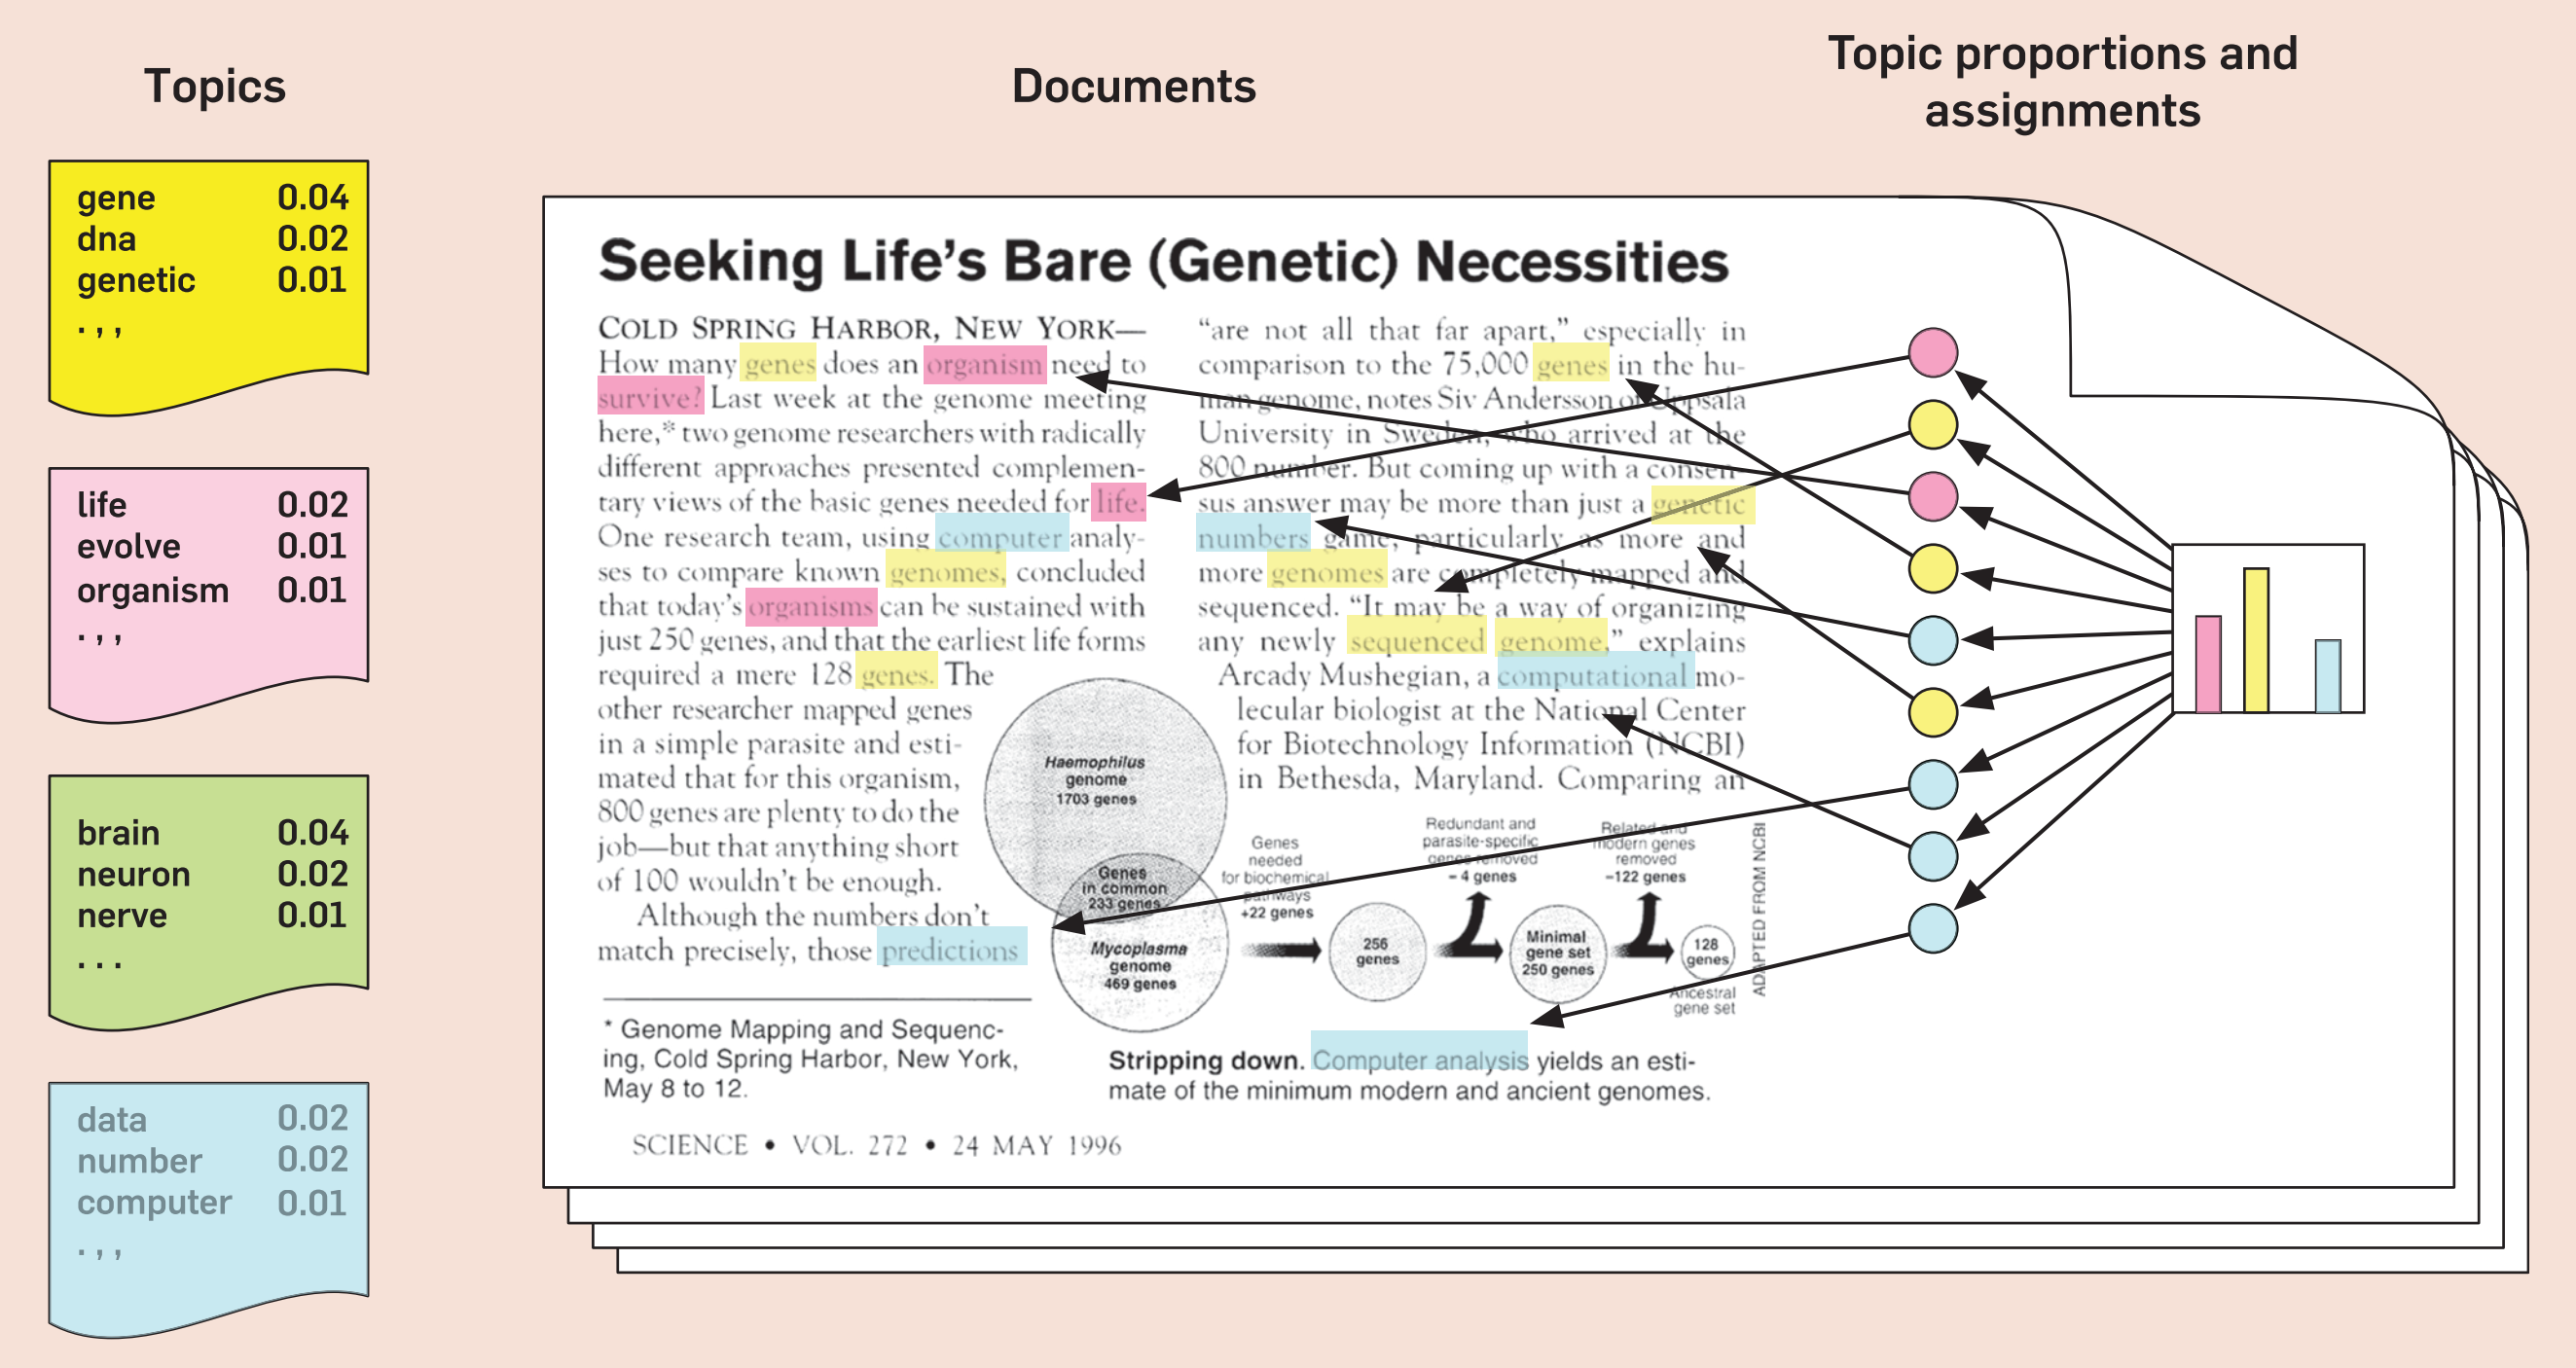
\includegraphics[width=1\textwidth]{figures/topicmodel}
    \caption{The intuition behind Latent Dirichlet Allocation. \cite{kim2019insider}}
\end{figure}
We assume that \textit{every document is a probability distribution over topics} (far right) and \textit{every topic is a probability distribution over words} (far left). The number of topics is a parameter defined by the user at initialization. 
We also assume that each document is generated by the following steps:
\begin{enumerate}
    \item Randomly choose a distribution over topics (the histogram on the right)
    \item Randomly choose the number of words for the document.
    \item For each word:
    \begin{enumerate}
        \item Randomly choose a topic (the colored coins)
        \item Randomly choose a word from the corresponding topic distribution (color from the coin matching the topic color on the left)
    \end{enumerate}
\end{enumerate}
To understand this process mathematically (see fig. \ref{fig:lda}), we reverse engineer a corpus. First, we assume a corpus has $M$ documents and a document has $N$ words $w_n$. The number of words is sampled from a poisson distribution $N\sim Poisson(\xi)$. Every word $w_n$ in a document is sampled from a multinomial distribution $\beta$ conditioned on the topic $z_n$. The topic $z_n$ is again sampled from a multinomial distribution $z_n\sim Multinomial(\theta)$. And at last, the multinomial distribution $Multinomial(\theta)$, that defines the topic distribution for a document, is sampled from a Dirichlet distribution: $\theta\sim Dir(\alpha)$. 
\begin{figure}[H]
    \centering
    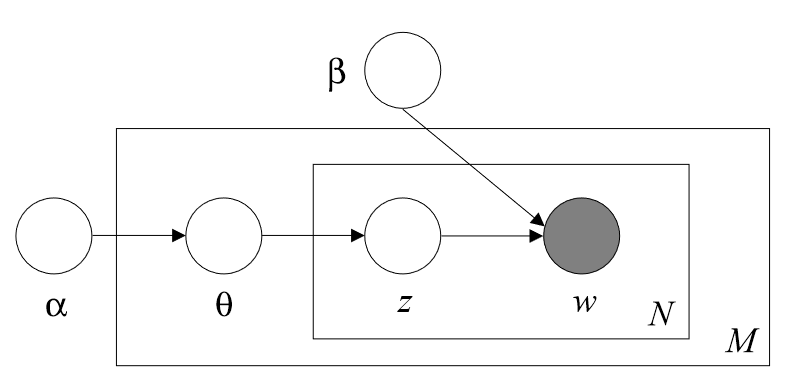
\includegraphics[width=0.8\textwidth]{figures/lda}
    \caption{Graphical model representation of the LDA model. \cite{blei2003latent}}
    \label{fig:lda}
\end{figure}

Simply speaking, if an LDA model is trained on a corpus, what we get are two sets of probability distributions. One set is the topic-word distribution where we get the multinomial distribution of words for every topic. The other is the multinomial distribution of topics for every document. 

With those two sets of distributions, we can make statements about what topics occur within our documents and what words those topics define. We can go even further, with LDA we can generate documents and therefore make assumptions what topics future documents might be about. 

However, a new document may contain words or topics that did not appear in any of the documents in the training corpus. These topics and words would have zero probability in the topic-word distribution. To smooth the multinomial parameters, the document-topic distribution is sampled from a Dirichlet distribution, but not the topic-word distribution. For this reason, we have to modify our LDA model. The modification as seen in fig. \ref{fig:lda_smooth} samples the multinomial topics-word distribution, $\beta$, also from a Dirichlet distribution $\beta\sim Dir(\eta)$.
\begin{figure}[H]
    \centering
    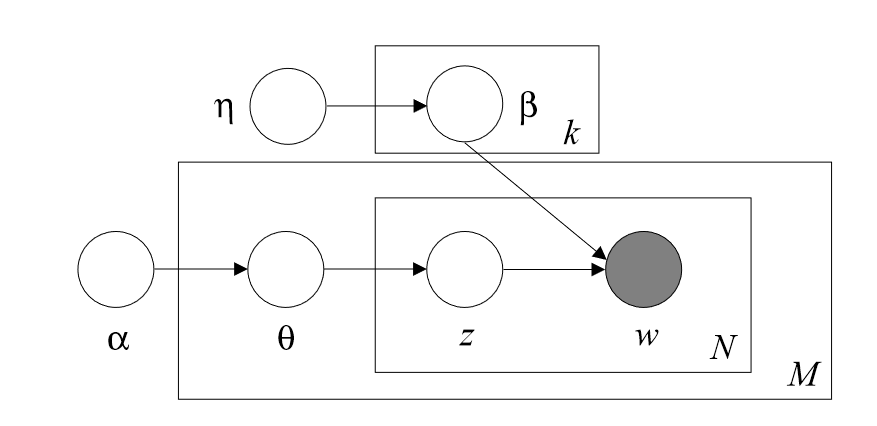
\includegraphics[width=0.8\textwidth]{figures/lda_smooth}
    \caption{Graphical model representation of the smoothed LDA model. \cite{blei2003latent}}
    \label{fig:lda_smooth}
\end{figure}
There are different strategies to train an LDA model. The original paper trains the LDA model through inference with variational Bayes \cite{blei2003latent} but since then there have been various other approaches, e.g. streaming Gibbs sampling \cite{gao2016streaming}, Markov random fields \cite{he2019end}, variational message passing \cite{taylor2021variational}, and many more.

In this work we are using LDA in combination with online variational Bayes \cite{hoffman2010online} which relies on online stochastic optimization. This technique manages to effortlessly analyze a massive amount of documents and can adapt to new documents at a later point in time without being trained from scratch.

% =======================================
\subsection{Neural LDA}
The parameters of the original LDA model have to be learned by variational inference techniques (e.g. EM algorithm for empirical Bayes, Gibbs sampling). This limits the model, especially for new data. Neural LDA proposes a new inference technique (AVITM) \cite{neuralLDA} that utilizes the inference network and does not require running slow variational optimization. To model a Dirichlet distribution with a neural network, they use a Laplace approximation \cite{mackay1998choice} so that the model prior could be assumed Gaussian. With that, the inference network can be defined as a neural network by using the reparametrization trick \cite{kingma2013auto} and the neural network is then able to successfully mimic the probabilistic inference process.  

% =======================================
\subsection{Evaluation and Metrics}
% =======================================
\subsubsection{Metrics of Quality (Topic Coherence)}\label{sec:coherence}
According to João Pedro \cite{topiccoherencemeasures}, topic modeling algorithms are a theoretical technique based on mathematics and statistics. However, a mathematically sound and perfect model does not necessarily reflect an ideal model from a human perspective. For example, a topic modeling algorithm containing the following two topics shows this problem.
\begin{enumerate}
    \item Topic: fish, shark, tuna, sea. \textit{(In our sense a good topic)}
    \item Topic: nurse, brick, cheese, dark. \textit{(In our sense rather a bad topic)}
\end{enumerate}
As a human, one might think the first topic contains more correlating words. On the other hand, for the algorithm, they are probably equal concerning correlating words. Considering our goal to understand data, we want topics that are human-friendly. Misleading and meaningless topics are a consequence of blindly trusting the algorithm. Topic coherence measures aim to put the quality of human perception about the created topics in a number to make the evaluation more feasible. Topic Coherence answers the question of how well a topic fits into a text considering the word combinations (the context) in it. This also means that the measure is not only dependent on the topic itself but also on the original text used for training the topic model. In general, we not only want to judge one topic but all generated topics. Therefore, we have to somehow combine all individual topic scores at the end. 

The topic coherence measure is defined in a pipeline-like structure (segmentation, probability calculation, confirmation measure, aggregation) as shown in fig. \ref{fig:tcm}. Each combination of those components uniquely defines different types of coherence scores. The reference corpus and the topics $t$ are received as inputs and a real valued confirmation measure $c$ is returned. 
\begin{figure}[H]
    \centering
    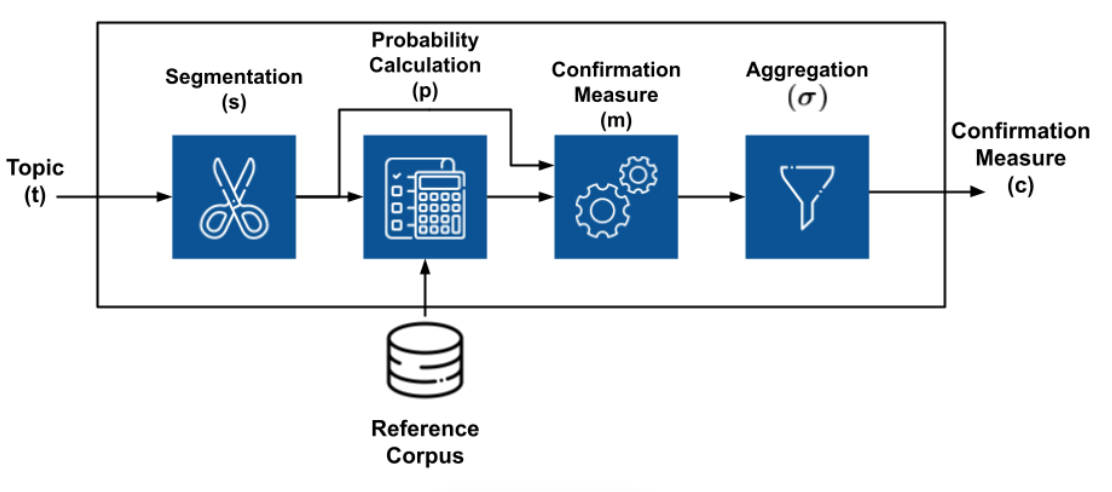
\includegraphics[width=0.9\textwidth]{figures/topiccoherence}
    \caption{General topic coherence measures structure. \cite{topiccoherencemeasures}}
    \label{fig:tcm}
\end{figure}
\textbf{The segmentation part} $s$ creates pairs of word subsets. For example, let $W={w_1,...,w_n}$ be the top-n most probable words of a topic $t$. Then, let $S$ be the set of subset pairs from $W$: $S={(W^{'},W^{*}),W^{'},W^{*}\subseteq W}$. $W^{*}$ is used to confirm $W^{'}$ in the probability calculation part. To get a better grasp of this segmentation let us look at some concrete examples for $W={"seal","egg","fibsh"}$:
\begin{equation}
    \begin{split}
        S^{one}_{one}(W)=\{&(seal,egg),(seal,fibsh),(egg,seal),\\
        & (egg,fibsh),(fibsh,seal),(fibsh,egg)\}
    \end{split}
\end{equation}
\begin{equation}
    \begin{split}
        S^{one}_{all}(W)=\{&(\{seal\},\{egg,fibsh\}),(\{egg\},\{seal,fibsh\}),\\
        & (\{fibsh\},\{seal,egg\})\}
    \end{split}
\end{equation}

\textbf{The probability calculation part} $p$ defines the function used to calculate the probabilities drawn from the corpus. Examples of such functions are the following:
\begin{itemize}
    \item \textbf{P}\textit{bd} (boolean document) calculates the probability as the number of documents the word or words $w$ occur in, divided by the total number of documents.
    \item \textbf{P}\textit{bs} (boolean sentence) calculates the probability as the number of sentences the word or words $w$ occur in, divided by the total number of sentences.
    \item \textbf{P}\textit{bsw} (boolean sliding window) calculates the probability as the number of sliding windows the word or words $w$ occur in, divided by the total number of sliding windows.
\end{itemize}
\textbf{The confirmation measure part} $m$ calculates a score by evaluating the probability function over the segmentations $S$ from the previous part. A low confirmation measure implicates that the words in $W^{'}$ are disconnected with the words in $W^{*}$ and vice versa (see fig. \ref{fig:tcp}). 
\begin{figure}[H]
    \centering
    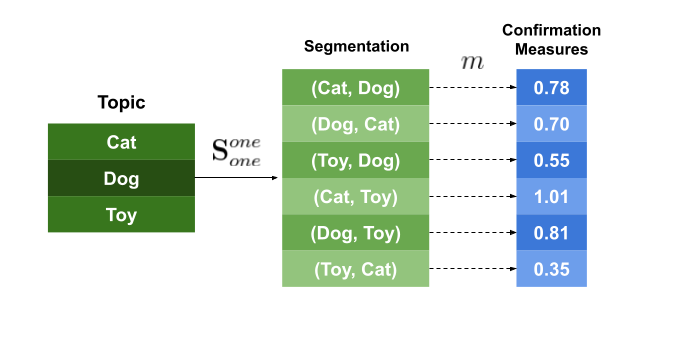
\includegraphics[width=0.9\textwidth]{figures/coherenceproba}
    \caption{Example of application of a confirmation measure $m$. \cite{topiccoherencemeasures}}
    \label{fig:tcp}
\end{figure}
There are two different types of confirmation measures:

\textit{Direct confirmation measures} use the subsets $W^{'}$ and $W^{*}$ to calculate the resulting score. E.g.:
\begin{equation}
    m_r(S_i)=\frac{P(W^{'},W^{*})}{P(W^{'})P(W^{*})}
\end{equation}
\begin{equation}
    m_{lr}(S_i)=log\frac{P(W^{'},W^{*})+\epsilon}{P(W^{'})P(W^{*})}
\end{equation}
\begin{equation}
    m_c(S_i)=\frac{P(W^{'},W^{*})}{P(W^{*})}
\end{equation}

\textit{Indirect confirmation measures} use the subset $W^{'}$ and $W^{*}$ separately to build a vector for all the words $W$ (see eq. \ref{eq:confmeas1}, \ref{eq:confmeas2}).
\begin{equation}
    \vec{v}_m(W^{'})=\left\{\sum_{w_i\in W^{'}}{m(w_i,w_j)}\right\}_{j=1,2,...,|W|}
    \label{eq:confmeas1}
\end{equation}
\begin{equation}
    \vec{v}_m(W^{'})=\left\{\sum_{w_i\in W^{'}}{m(w_i,w_j)}\right\}_{j=1,2,...,|W|}
    \label{eq:confmeas2}
\end{equation}
Those two vectors are combined with, for example, the cosine similarity function (see eq. \ref{eq:cos}).
\begin{equation}
    \tilde{m}_{cos}(W^{'},W^{*})=s_{cos}(\vec{v}_m(W^{'}),\vec{v}_m(W^{*}))
    \label{eq:cos}
\end{equation}
The idea behind the indirect confirmation measure is to find relations that the direct method could not.

\textbf{The aggregation part} $\sigma$ combines all previously calculated values into one. This value is the final topic coherence score and can be, for example, the arithmetic mean.

Currently, the score that has the highest correlation with all available human topic-ranking data is the coherence score $C_v$ \cite{syed2017full}. The type of the coherence score, as mentioned before, is uniquely defined by the segmentation, the probability calculation, the confirmation measure and the aggregation:
\begin{itemize}
    \item $S_{set} = \{(W', W^{*})\mid W' = \{w_i\}; w_{i} \in W; W^{*} = W\}$
    \item \textbf{P}\textit{bsw} - Boolean Sliding Window
    \item $\phi_{S_i}(\vec{u},\vec{w})=\frac{\sum_{i=1}^{|W|}{\vec{u}_i}\cdot\vec{w}_i}{\|\vec{u}\|_2\cdot\|\vec{w}\|_2},\;$ with $\;
           \vec{v}(W^{'})=\left\{\sum_{w_i\in W^{'}}{\textbf{NPMI}(w_i,w_j)^{\gamma}}\right\}_{j=1,...,|W|}\;$ and 
            $\;\textbf{NPMI}(w_i,w_j)^{\gamma}=\left(\frac{\text{log}\frac{P(w_i,w_j)+\epsilon}{P(w_i)\cdot P(w_j)}}{-\text{log}(P(w_i,w_j)+\epsilon}\right)$
    \item $\sigma=$ The arithmetic mean
\end{itemize}

A full insight in topic coherence measures with more examples of each part can be found in \textit{Exploring the Space of Topic Coherence Measures} by Röder et al. \cite{roder2015exploring}

% =======================================
\subsubsection{Metrics of Differences Between Models (Distance)}\label{sec:diffmet}
Topic models generate probability distributions and one way to compare those models with each other is to measure the similarity between them. We can do this by using the Jensen-Shannon distance. The Jensen-Shannon distance is the square root of the Jensen-Shannon divergence, also known as the information radius or total divergence to the average. The Jensen-Shannon divergence \cite{fuglede2004jensen} is based on the Kullback-Leibler divergence ($D_{KL}$) with the difference that it is symmetric and it always has a finite value. 
\begin{equation}
    JSD(P||Q)=\frac{1}{2}D_{KL}\left(P\left|\left|\frac{1}{2}(P+Q)\right.\right.\right)+\frac{1}{2}D_{KL}\left(Q\left|\left|\frac{1}{2}(P+Q)\right.\right.\right),
\end{equation}
with $D_{KL}(P||Q)$ denoting the relative entropy of $P$ with respect to $Q$.

The more similar the two distributions $P$ and $Q$ are, the closer to zero the resulting value is. The evaluation between two topic models requires both to have been trained with the same vocabulary. The vocabularies have to be exactly the same, including the positions of the words. Otherwise, additional and very tedious coding is required.

Furthermore, the topics of two topic models are not guaranteed to match the same topic IDs (1-1, 2-2, etc.). Therefore, the result is going to be a matrix ($M_{i,j}$ with $i,j\in[0,...,t]$, where $t=\textit{num topics}-1$), where all topics are compared to each other. The matching topics are then found by the lowest score for every line (or row). 
\chapter{Problem Statement}\label{chp:problemstatement}
\chapter{Experiments}\label{chp:experiments}
In this chapter we explain the implementation of our proposed approach and show the results we obtained. The git repository can be accessed here \cite{gitrepo}.

% =======================================
\section{Setup}
% =======================================
\subsection{Training Language Models}
To train our own language models we are using the HuggingFace library \cite{huggingface} implemented in Python for reproducibility. We use the predefined model parameters for both models (GPT-2 \cite{gpt2model}, Transformer-XL \cite{trafoxlmodel}) and train them on the Wikitext103 \cite{merity2016pointer,wikitext} corpus.\footnote{In this section, the terms "dataset" and "corpus" are used interchangeably.} To provide optimal results, we remove all headers and titles from the corpus previous to the training. The training itself is done on the ETH supercomputer Euler \cite{euler} on one \texttt{NVIDIA V100 TENSOR CORE GPU}. We name our new models \texttt{"gpt2\_ours"} and \texttt{"trafo\_xl\_ours"}. After training we evaluate our models using the perplexity score (see sec. \ref{sec:perplexity}) as implemented in the HuggingFace library and compare them to the scores from the original paper. 

\subsection{Generating Corpora}
We are conducting our analysis on a total of 32 different corpora with sizes of 10'000 and 100'000 documents. The 32 corpora also include duplicates which are created by sampling with a different seed, resulting in the two identifiers \texttt{dataset1} (seed $=42$) and \texttt{dataset2} (seed $=1337$). To create a document, we sample word tokens from a language model. We start with the BOS token (or empty string) and sample until the EOS token appears or until the string length of $1024$ characters is reached. 

From the already existing and preprocessed corpus Wikitext103, we randomly draw (with replacement) 10'000 and 100'000 documents. We do the same with the ArXiv corpus, where we only use the abstracts.
\begin{multicols}{2}
\begin{itemize}
    \item \texttt{dataset1-Wikitext103-10000}
    \item \texttt{dataset1-Wikitext103-100000}
    \item \texttt{dataset1-ArXiv-10000}
    \item \texttt{dataset1-ArXiv-100000}
    \item \texttt{dataset2-Wikitext103-10000}
    \item \texttt{dataset2-Wikitext103-100000}
    \item \texttt{dataset2-ArXiv-10000}
    \item \texttt{dataset2-ArXiv-100000}
\end{itemize}
\end{multicols}
From the original pretrained GPT-2 model, we sample 100'000 documents with ancestral sampling. For the smaller subset of 10'000 documents, we just take the first 10'000 entries from the larger set. The Transformer-XL model requires more computation power than GPT-2 to sample from. We therefore limit our corpus to 10'000 samples.
\begin{multicols}{2}
\begin{itemize}
    \item \texttt{dataset1-gpt2-10000}
    \item \texttt{dataset1-gpt2-100000}
    \item \texttt{dataset1-trafo\_xl-10000}
    \item \texttt{dataset2-gpt2-10000}
    \item \texttt{dataset2-gpt2-100000}
    \item \texttt{dataset2-trafo\_xl-10000}
\end{itemize}
\end{multicols}
From our own trained GPT-2 model (\texttt{gpt2\_own}), we sample 100'000 documents with ancestral sampling, Top-P sampling and Typical sampling (see sec. \ref{sec:sampling}). For the 10'000 document corpus we take again the first 10'000 documents from the respective larger corpus. We do the same for our self trained Transformer-XL model (\texttt{trafo\_xl\_own}) but limit the corpus size again to 10'000 samples. 
\begin{multicols}{2}{\footnotesize
\begin{itemize}
    \item \texttt{dataset1-gpt2\_ours-10000}
    \item \texttt{dataset1-gpt2\_ours-100000}
    \item \texttt{dataset1-gpt2\_ours-top\_p-10000}
    \item \texttt{dataset1-gpt2\_ours-top\_p-100000}
    \item \texttt{dataset1-gpt2\_ours-typ\_p-10000}
    \item \texttt{dataset1-gpt2\_ours-typ\_p-100000}
    \item \texttt{dataset1-trafo\_xl\_ours-10000}
    \item \texttt{dataset1-trafo\_xl\_ours-top\_p-10000}
    \item \texttt{dataset1-trafo\_xl\_ours-typ\_p-10000}
    \item \texttt{dataset2-gpt2\_ours-10000}
    \item \texttt{dataset2-gpt2\_ours-100000}
    \item \texttt{dataset2-gpt2\_ours-top\_p-10000}
    \item \texttt{dataset2-gpt2\_ours-top\_p-100000}
    \item \texttt{dataset2-gpt2\_ours-typ\_p-10000}
    \item \texttt{dataset2-gpt2\_ours-typ\_p-100000}
    \item \texttt{dataset2-trafo\_xl\_ours-10000}
    \item \texttt{dataset2-trafo\_xl\_ours-top\_p-10000}
    \item \texttt{dataset2-trafo\_xl\_ours-typ\_p-10000}
\end{itemize}}
\end{multicols}

% ====================================
\subsection{Training Topic Models}

% ====================================
\subsubsection{Additional Preprocessing}
Before training our topic models, we do some preprocessing on our datsets to tokenize our documents:
\begin{enumerate}
    \item convert every character to lowercase
    \item split strings into words
    \item remove numbers, but not words that contain numbers
    \item remove words that contain only one character
    \item lemmatize the document
    \item (optional) add bigrams and append to each document
    \item (optional) add trigrams and append to each document
\end{enumerate}
We test the influence of unigrams, the combination of unigrams and bigrams, and the combination of unigrams, bigrams and trigrams on all of our results. 

% ====================================
\subsubsection{Dictionary Creation} 
After preprocessing, we create a dictionary for each corpus and filter all words that appear in more than 50\% of the documents or appear less than 20 times. 

As we want to compare two corpora with each other, we are required to use the same dictionary in the exact same order when creating the topic models. Therefore, each comparing pair has their unique dictionary. We create two versions of that dictionary, one where we take the intersection and one where we take the union of the two original dictionaries.

% ====================================
\subsubsection{Training Topic Models}
For creating topic models with classic LDA, we use the \texttt{LdaMulticore} class from the Gensim library \cite{gensim}. We are training the model on the ETH Euler supercomputer, each model on 4 cores. We find that a higher core count does not give us any increase in performance. To evaluate the stability of the LDA model, we train 9 additional topic models of the same topic with a different seed for the \texttt{gpt2\_ours}, \texttt{Wikitext103} and \texttt{ArXiv} corpora with both 10'000 and 100'000 documents.

For creating topic models with neural LDA \cite{neuralLDA}, we use the OCTIS library \cite{octis}. Due to hardware and software limitations, we limit the training size to 10'000 samples. We train all neural LDA models on the ETH Euler supercomputer on an \texttt{NVIDIAGeForceGTX1080} each. As the neural LDA model is a neural network, we find the optimal hyperparameter by using Bayesian optimization. There, we find that a low dropout rate ($\le0.2$), a low number of layers ($\leq2$) and a higher number of neurons ($\geq1800$) result in optimal models.

We train topic models for 2, 3, 5, 10, 20, 50 and 100 topics and evaluate them using the $C_v$ coherence score (see sec. \ref{sec:coherence}).

% =======================================
\subsection{A Metric for Comparing Topic Models}
The results of a topic model are two sets of probability distributions, the topic-word and document-topic distribution matrices. We are interested in how similar topics from different models are. Similar topics can be understood as two topic-word distributions with a similar set of highly probable words (see fig. \ref{fig:wordcloud-gpt2_nt-wiki_nt-5-2} and \ref{fig:wordcloud-gpt2_nt-wiki_nt-10-3}). 
\begin{figure}[H]
    \centering
    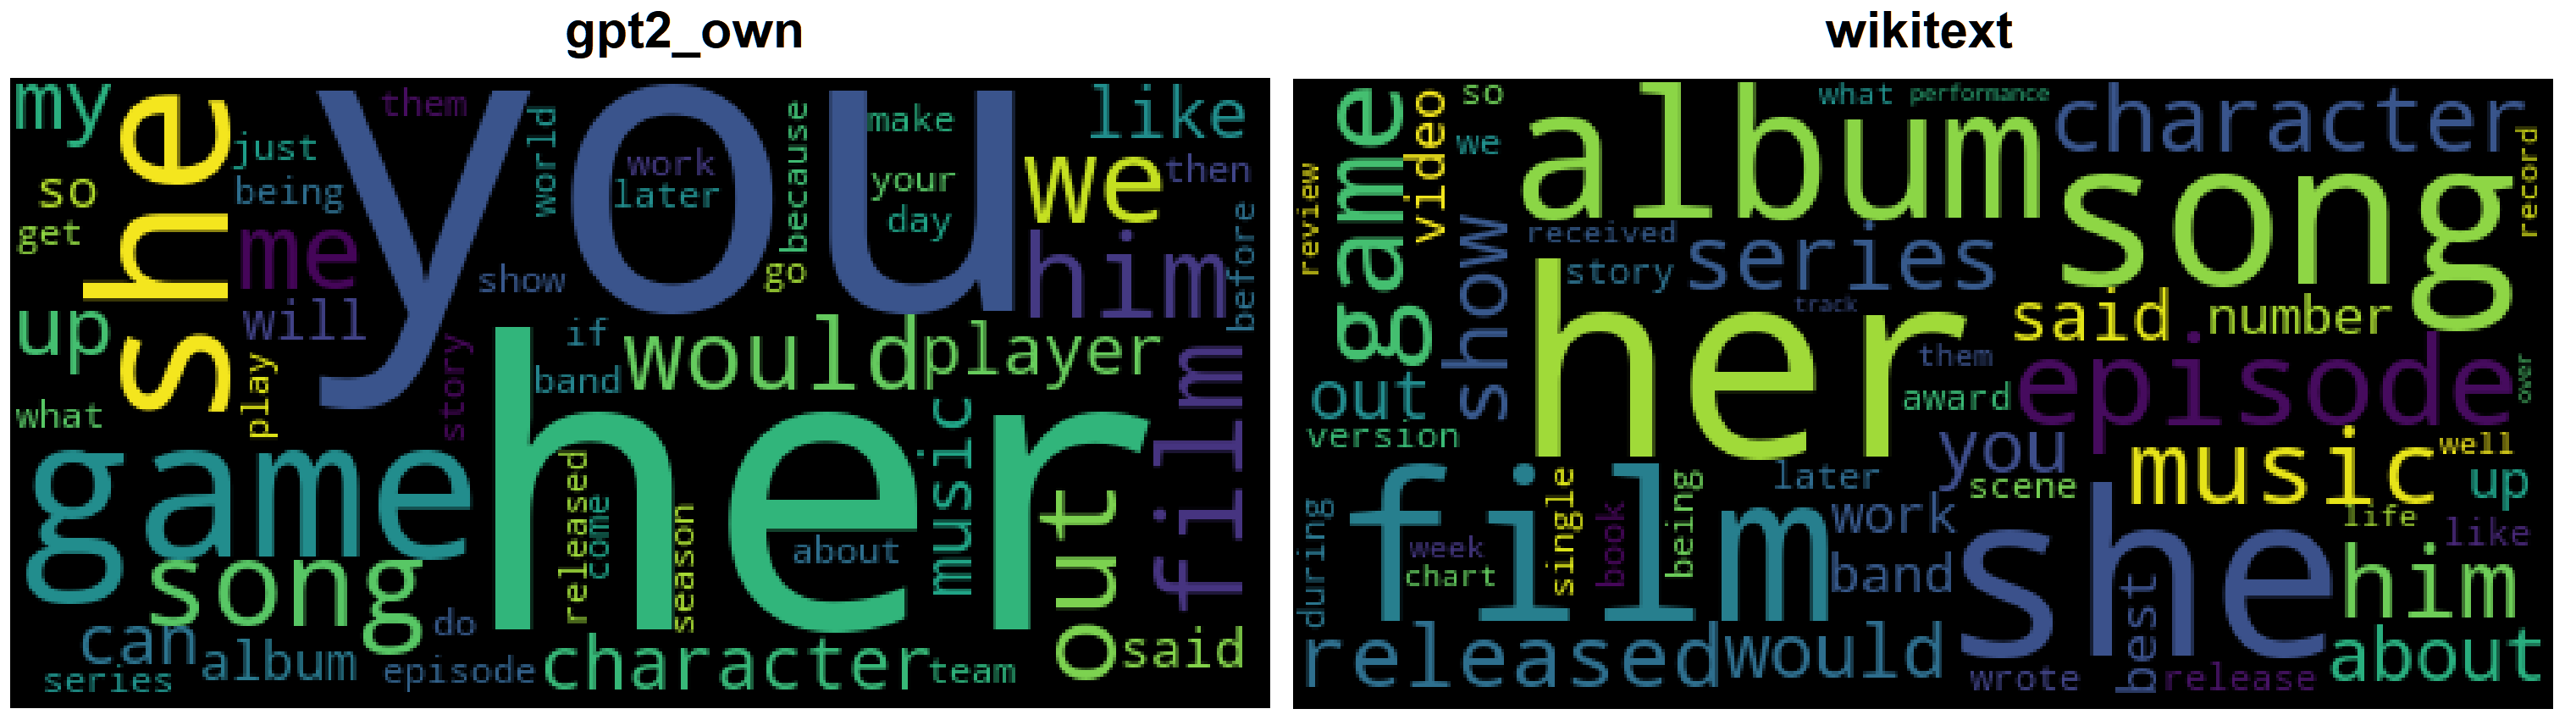
\includegraphics[width=0.8\textwidth]{figures/wordcloud-gpt2_nt-wiki_nt-5-2}
    \caption{Wordcloud example 1 of two similar topics. The size of the word corresponds to the probability of that word in that topic. This is topic 2 out of 5, trained on a corpus with 100'000 documents, using intersected dictionaries and ancestral sampling. Created using classic LDA.}
    \label{fig:wordcloud-gpt2_nt-wiki_nt-5-2}
\end{figure}
\begin{figure}[H]
    \centering
    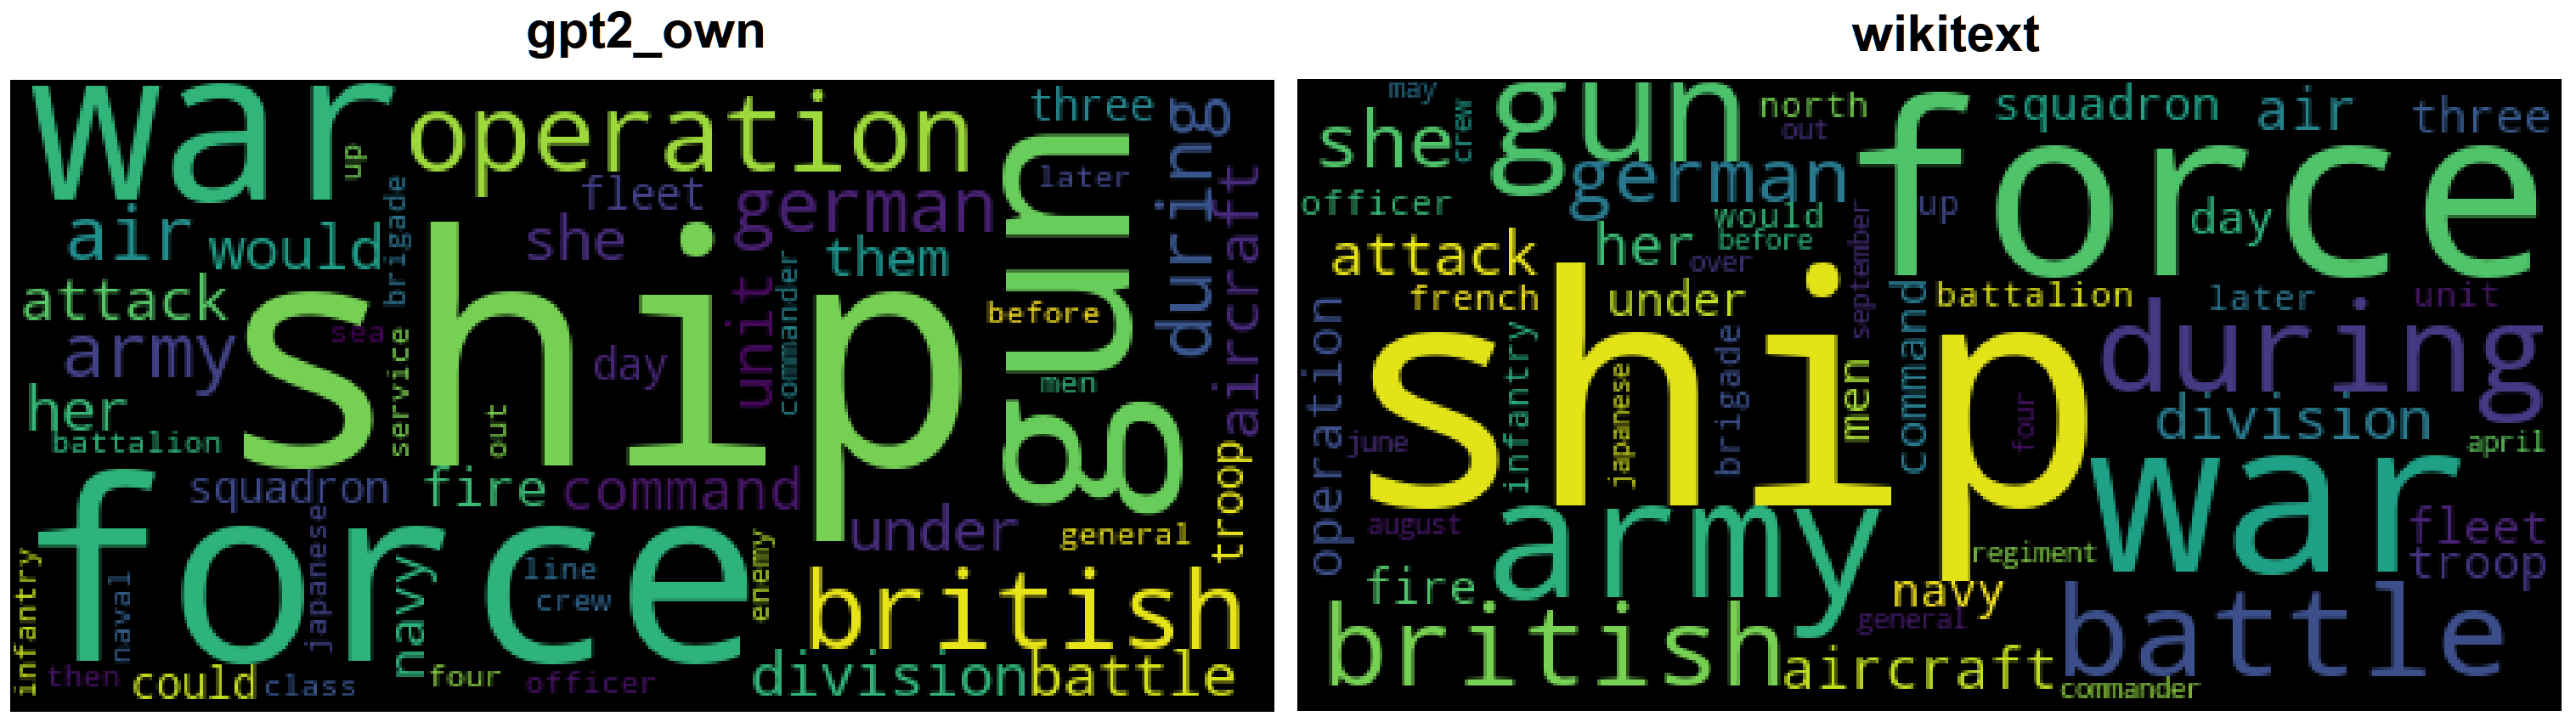
\includegraphics[width=0.8\textwidth]{figures/wordcloud-gpt2_nt-wiki_nt-10-3}
    \caption{Wordcloud example 2 of two similar topics. The size of the word corresponds to the probability of that word in that topic. This is topic 3 out of 10, trained on a corpus with 100'000 documents, using intersected dictionaries and ancestral sampling. Created using classic LDA.}
    \label{fig:wordcloud-gpt2_nt-wiki_nt-10-3}
\end{figure}
To put that comparison into a number, we compare all rows from the topic-word matrices $T_1$ and $T_2$ with each other by using the Jensen-Shannon distance. The rows contain the topic-word distributions of the words. We then obtain two new matrices $M^{(1)}$ and $M^{(2)}$ (see eq. \ref{eq:jsd}) containing those distances for every topic pair.
\begin{equation}\label{eq:jsd}
    \begin{split}
        & M^{(1)}_{i,j}=JSD(P_i||Q_j), \\
        & M^{(2)}_{i,j}=JSD(Q_i||P_j),\\
        & \forall i,j\in[0,n-1],\\
        & n = \text{number of topics,}\\
        & P_i=i-th \text{ row of }T_1,\\
        & Q_j=j-th \text{ row of }T_2
    \end{split}
\end{equation}
Fig. \ref{fig:diff_classic_lda_intersection_5} and \ref{fig:diff_classic_lda_intersection_10} are illustrations of similarity matrices. A deep dark red means that two topics are very different and a deep dark blue indicates the opposite. As shown, not every topic from one model has a matching counterpart. Occasionally, there are multiple topics from the other topic model that are similar to one topic. 
\begin{figure}[H]
    \centering
    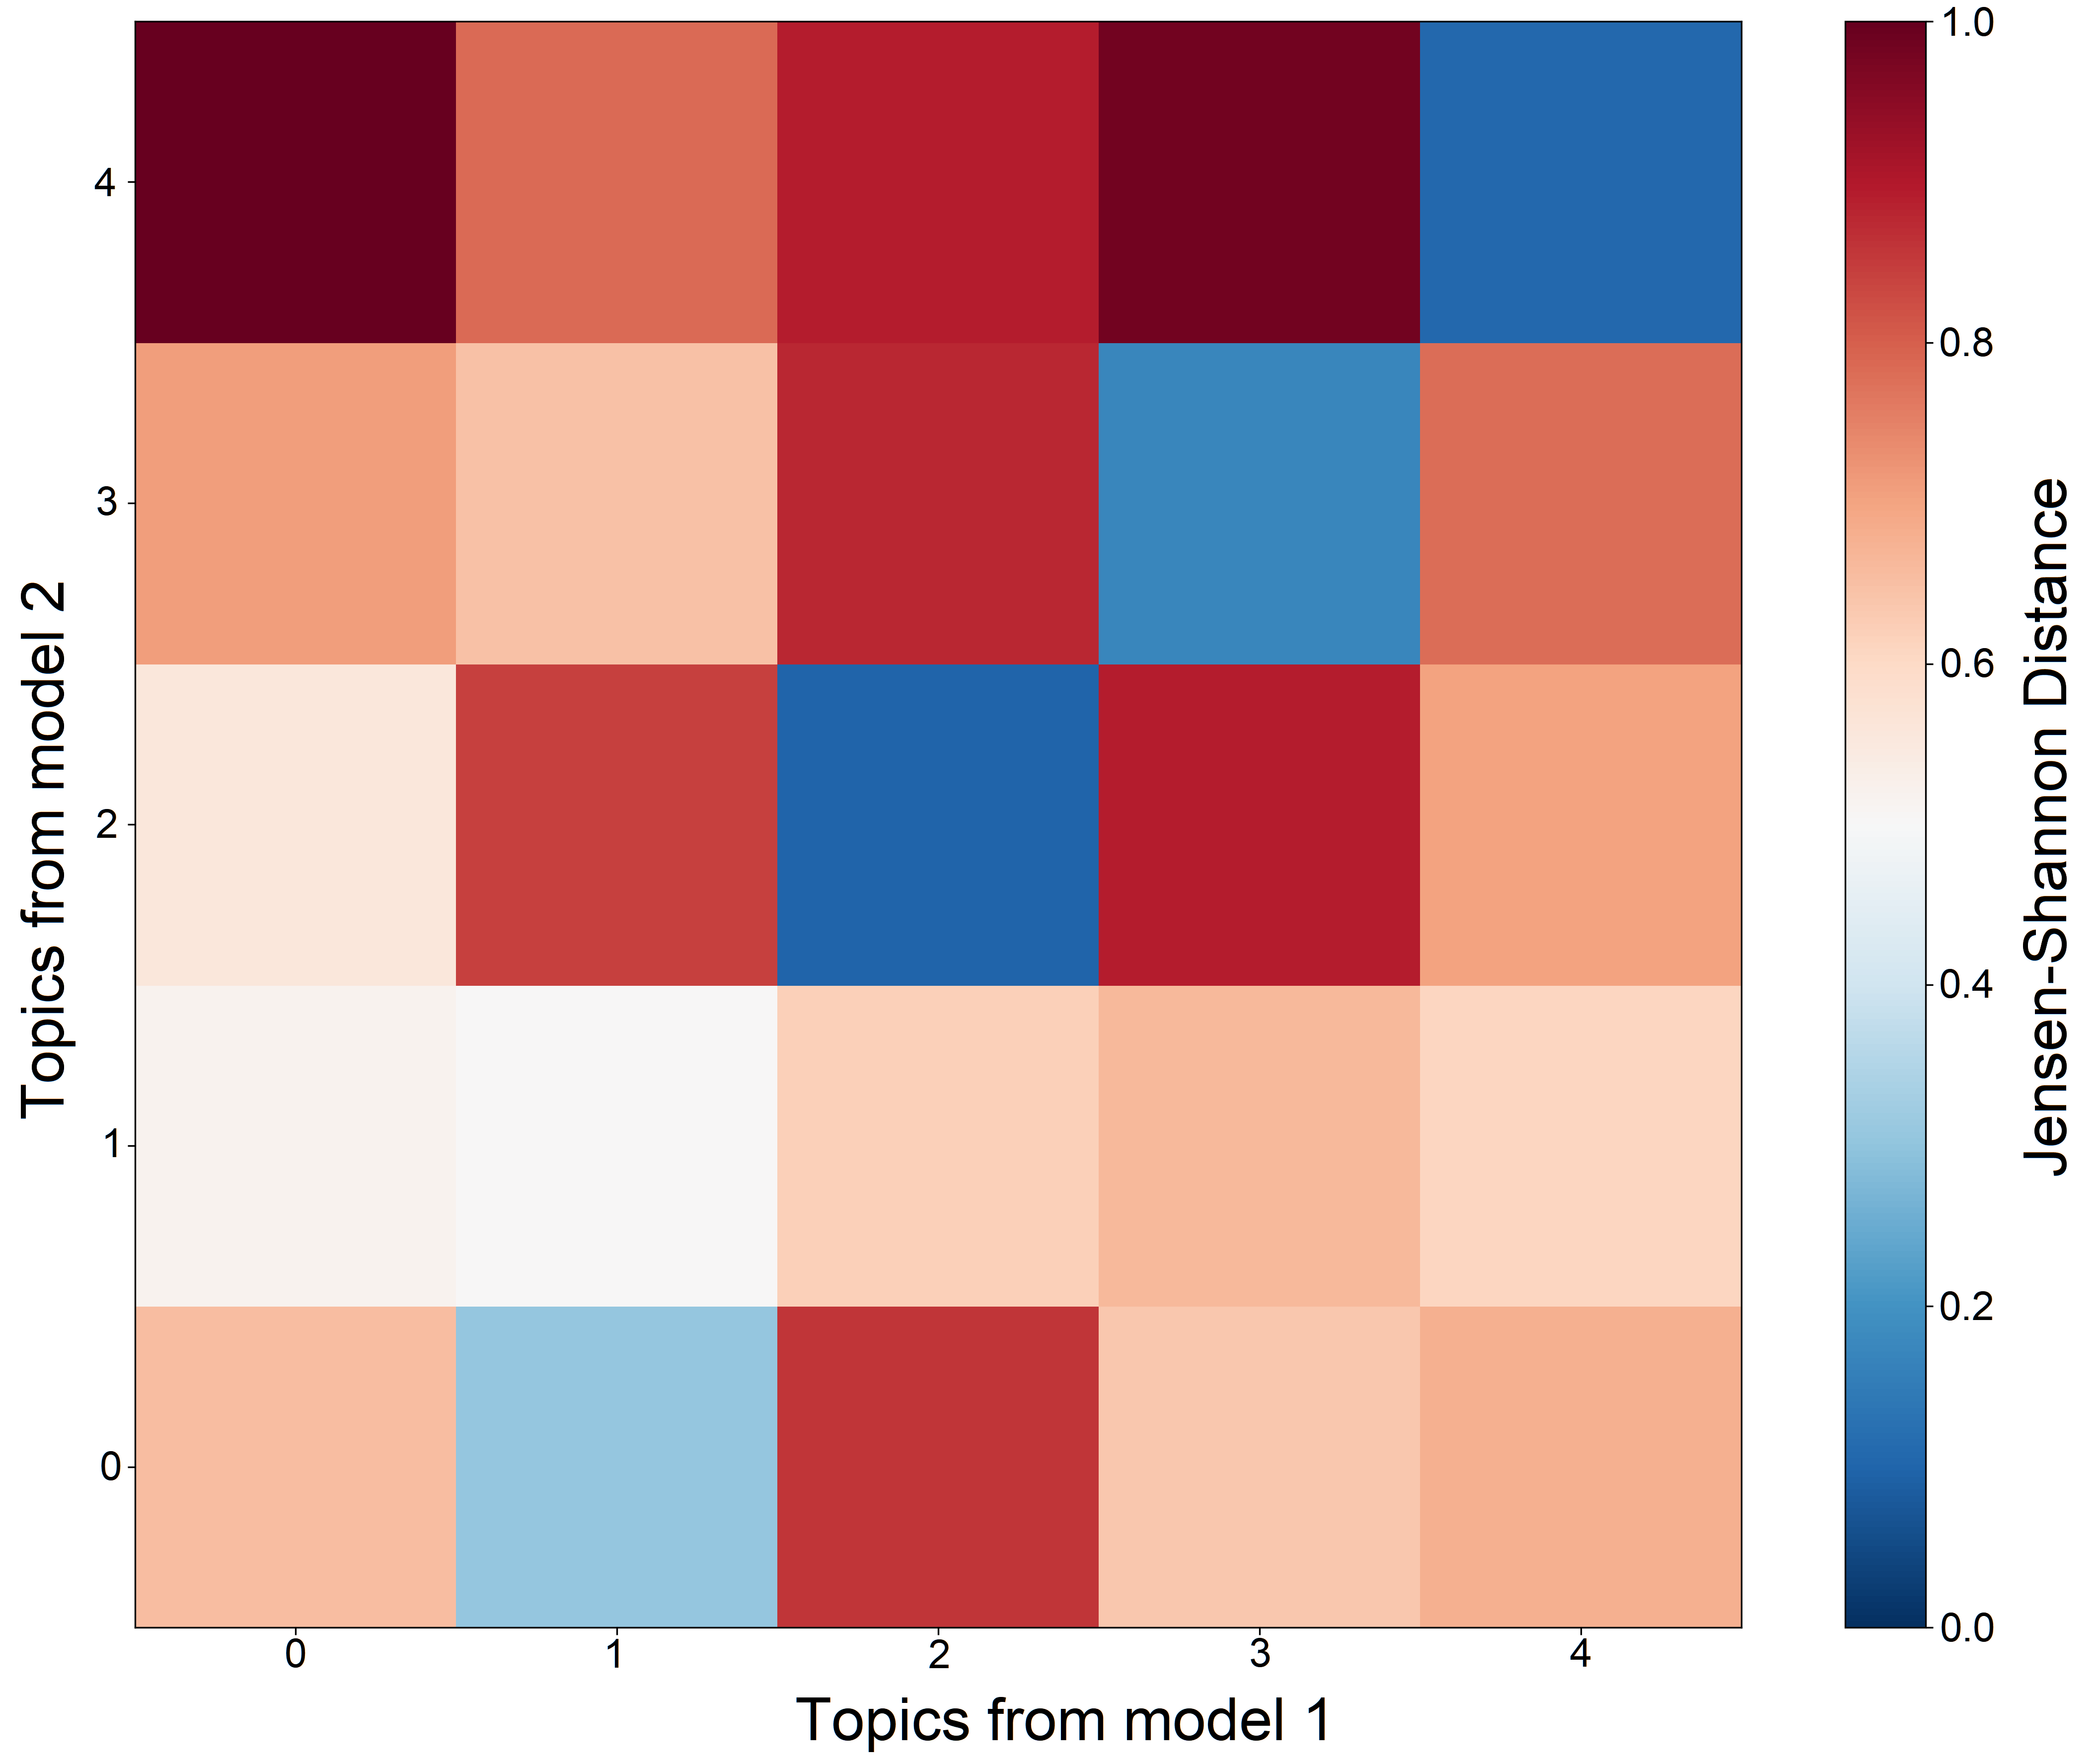
\includegraphics[width=0.5\textwidth]{figures/diff_classic_lda_intersection_5}
    \caption{Illustration of the similarity matrix for 5 topics using the Jensen-Shannon distance. Comparing \texttt{gpt2\_ours} vs. \texttt{wikitext}, trained on a corpus size of 100'000 documents and with intersected dictionaries.}
    \label{fig:diff_classic_lda_intersection_5}
\end{figure}
\begin{figure}[H]
    \centering
    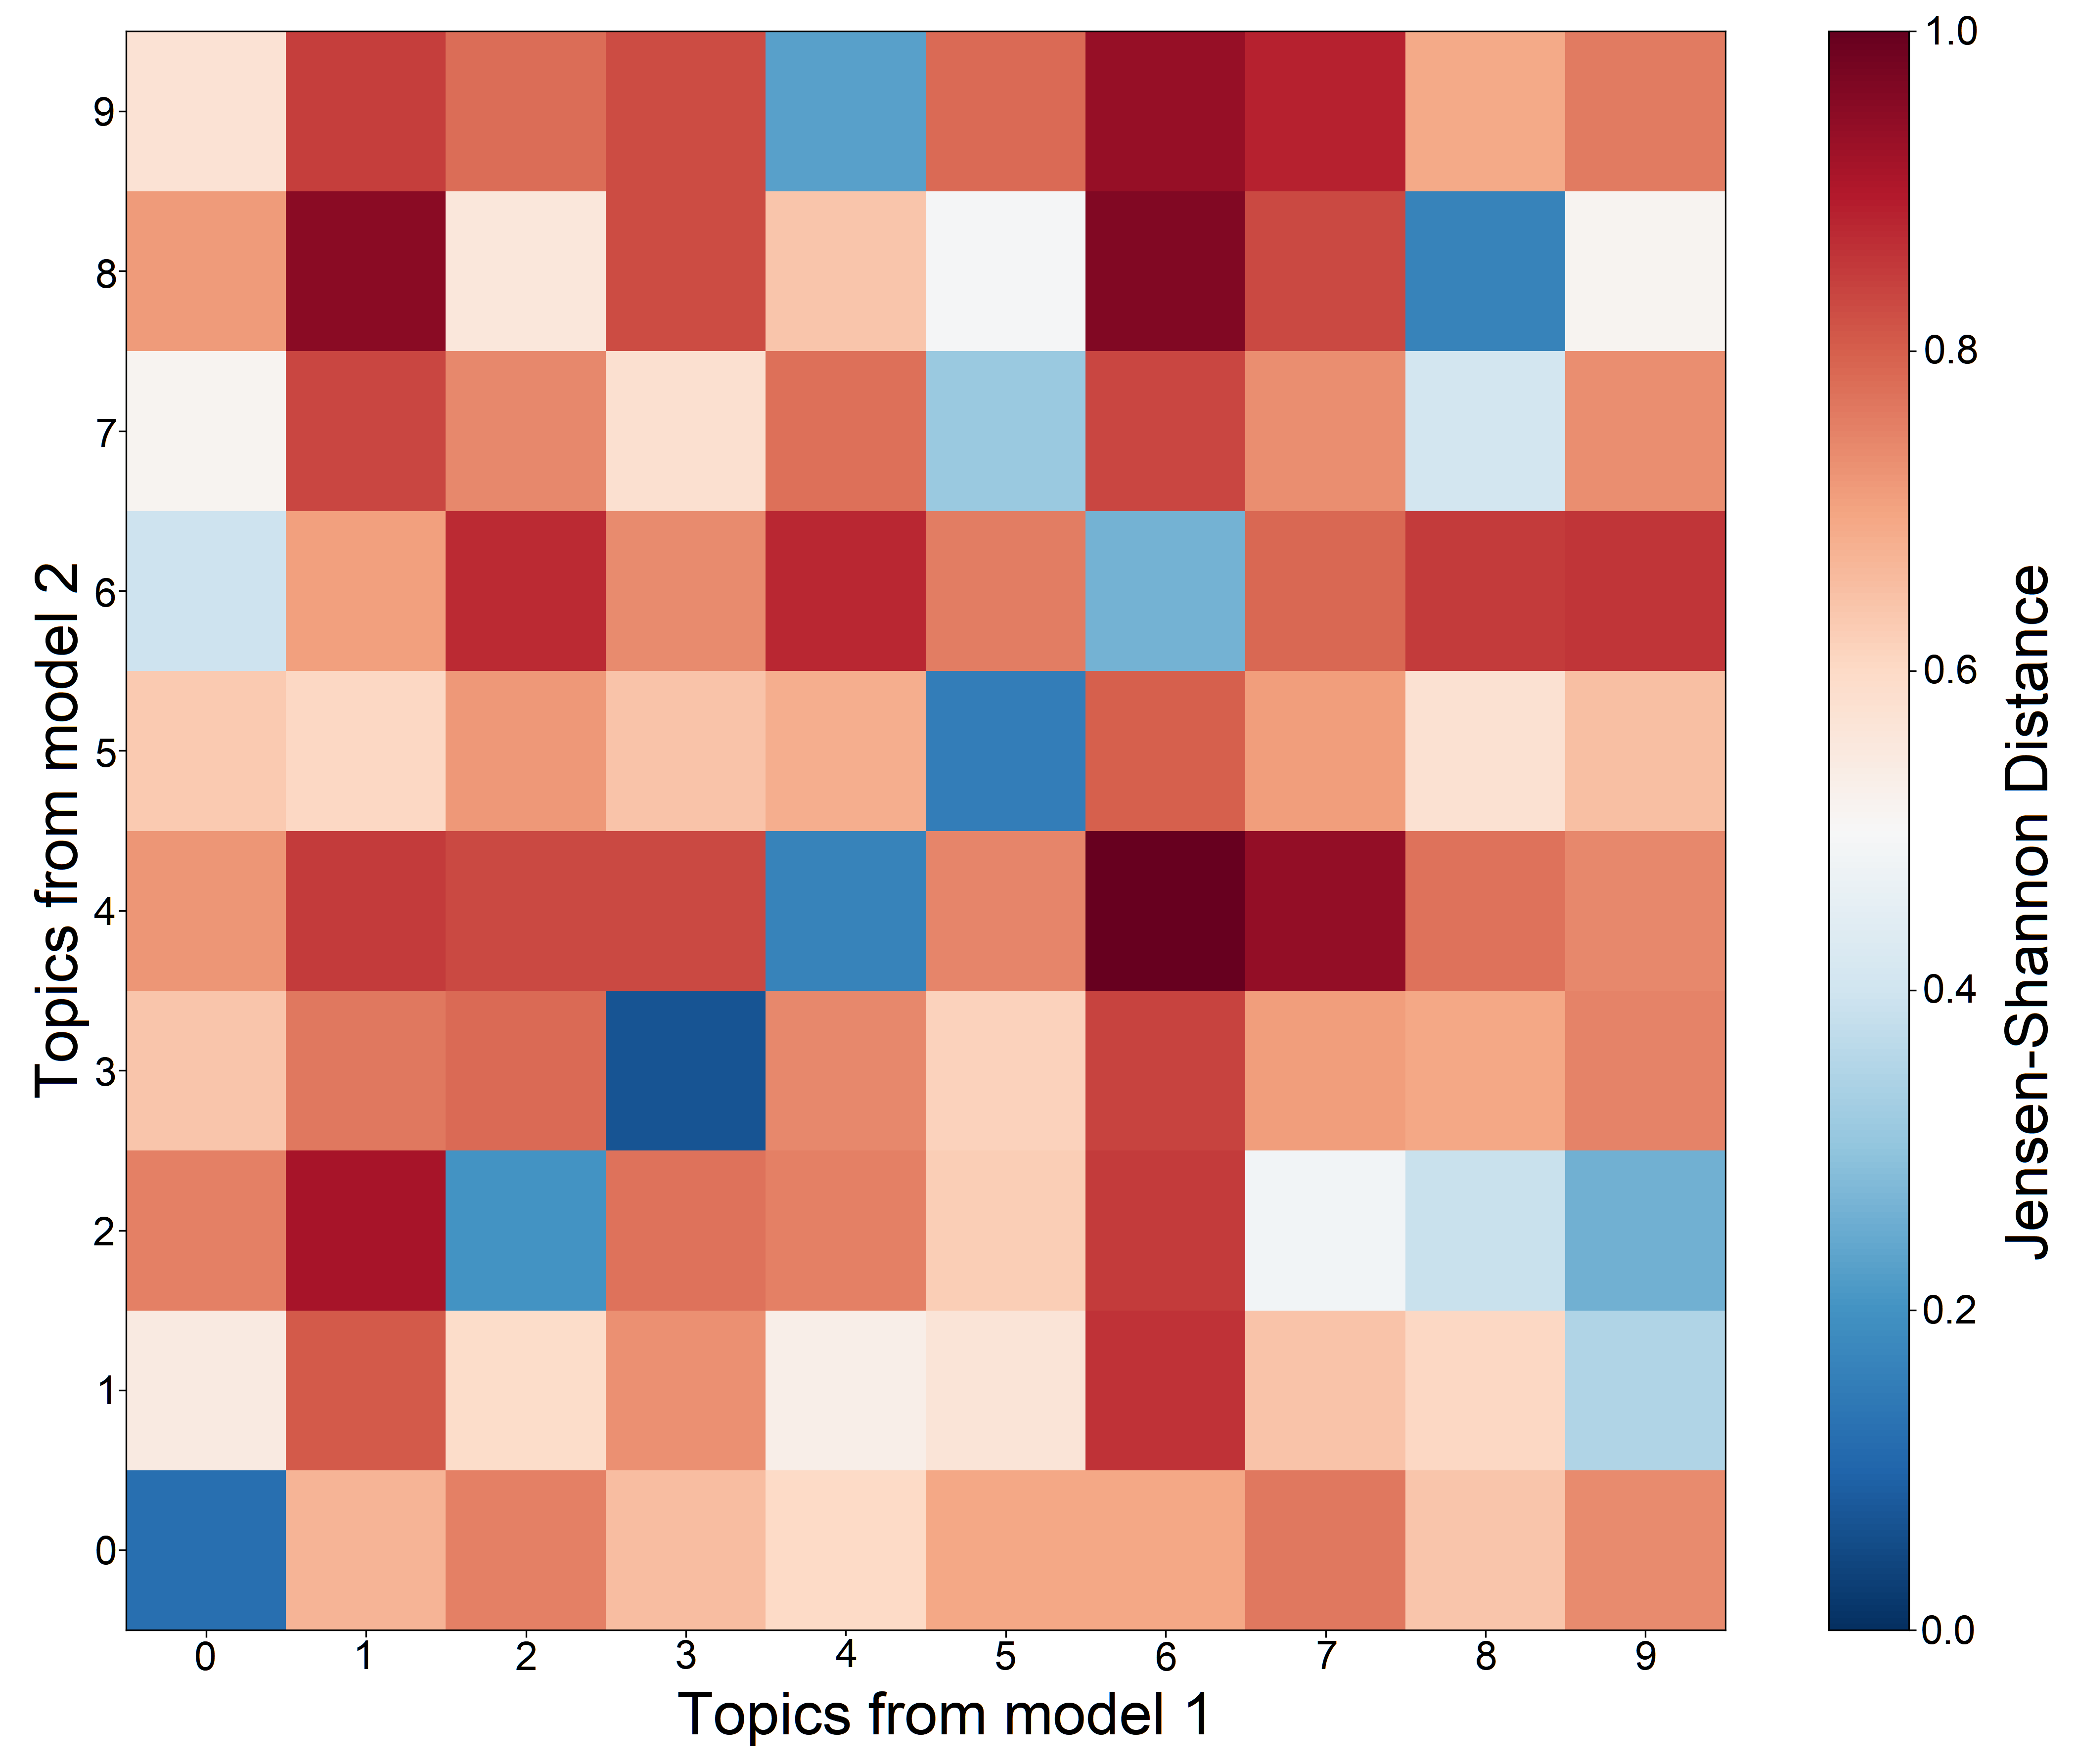
\includegraphics[width=0.6\textwidth]{figures/diff_classic_lda_intersection_10}
    \caption{Illustration of the similarity matrix for 10 topics using the Jensen-Shannon distance. Comparing \texttt{gpt2\_ours} vs. \texttt{wikitext}, trained on a corpus size of 100'000 documents and with intersected dictionaries.}
    \label{fig:diff_classic_lda_intersection_10}
\end{figure}
In order to find out if two topic models found similar clusters, we take the best match for each topic and weigh it by how probable that topic is in the corpus. For this, we calculate the boolean probability of each topic. Meaning, for a topic, we count the number of times it is the most dominant topic in a document, divided by the total number of documents in a corpus. With the two document-topic matrices $D1$ and $D2$, we get the Python code snippet in \ref{eq:probabpython}.
\begin{code}
\captionof{listing}{Topic Probability Calculation}
\label{eq:probabpython}
\begin{minted}{Python}
    import numpy as np
    
    n = number_of_topics
    m = total_numer_of_documents
    u1 = np.argmax(D1, axis=1)  
    u2 = np.argmax(D2, axis=1)
    p1 = np.zeros(n)
    p2 = np.zeros(n)
    
    for topic in range(n):
        p1[topic] = np.count_nonzero(u1 == topic)/m
        p2[topic] = np.count_nonzero(u2 == topic)/m
\end{minted}
\end{code}
Now, we weigh the resulting vector from taking the minimum in every row from the similarity matrix with the probability vector and sum them up. We combine those two operations with the scalar product. Our final metric is the mean of both resulting values as shown in eq. \ref{eq:final}.  
\begin{equation}\label{eq:final}
    \text{metric }=\frac{\langle p1,\text{ amin}(M^{(1)},\text{ axis}=1)\rangle + \langle p2,\text{ amin}(M^{(2)},\text{ axis}=1)\rangle}{2}
\end{equation}

% =======================================
\section{Results}\label{sec:results}
During our experimentation we find that topic models created with intersected dictionaries tend to be more reliable and stable in relation to our metric and the quality of the topic models. We therefore focus our findings on results with intersected dictionaries. Furthermore, we did not find any notable difference in our results by adding bigrams or trigrams to our dictionaries, thus we only report on our findings with unigrams.

% =======================================
\subsection{Quality of Our Language Models}
Concerning the quality of our language models, we do not see a major deviation from the original scores (see table \ref{tab:origcoh}) and can therefore say that the quality of our language models is in the range of confidence of the original scores. This means that we assume our trained language models have learned the language of the corpus they were trained on to the same degree as the original models.
\begin{table}[ht]
\caption{Perplexity}
\centering
    \begin{tabular}{ |p{3cm}||p{3cm}|p{3cm}|  }
        \hline
        Language Model & Original & Ours\\
        \hline
        \hline
        GPT-2          & 37.50 & 32.58\\
        \hline
        Transformer-XL & 24.0  & 27.43\\
        \hline
    \end{tabular}
\label{tab:origcoh}
\end{table}

% =======================================
\subsection{Quality of Our Topic Models}
% =======================================
\subsubsection{Corpora With 100'000 Samples}
For corpora with 100'000 documents, we evaluate the coherence score (mean and variance) in two ways for each corpus (\texttt{gpt2\_ours}, \texttt{gpt2}, \texttt{wikitext}, \texttt{arxiv}). First, we compare the influence of changing the seed when creating a topic model. The mean and variance is taken from topic models with different seeds. As shown in fig. \ref{fig:Unigrams-100000-var-cv-is}, the mean ranges from $0.33$ to $0.58$ and the variance stays in the range of $\pm0.05$ of the mean. On average, we can see that the quality of each of our topic models here is the highest when using $20$ to $50$ topics.
\begin{figure}[H]
    \centering
    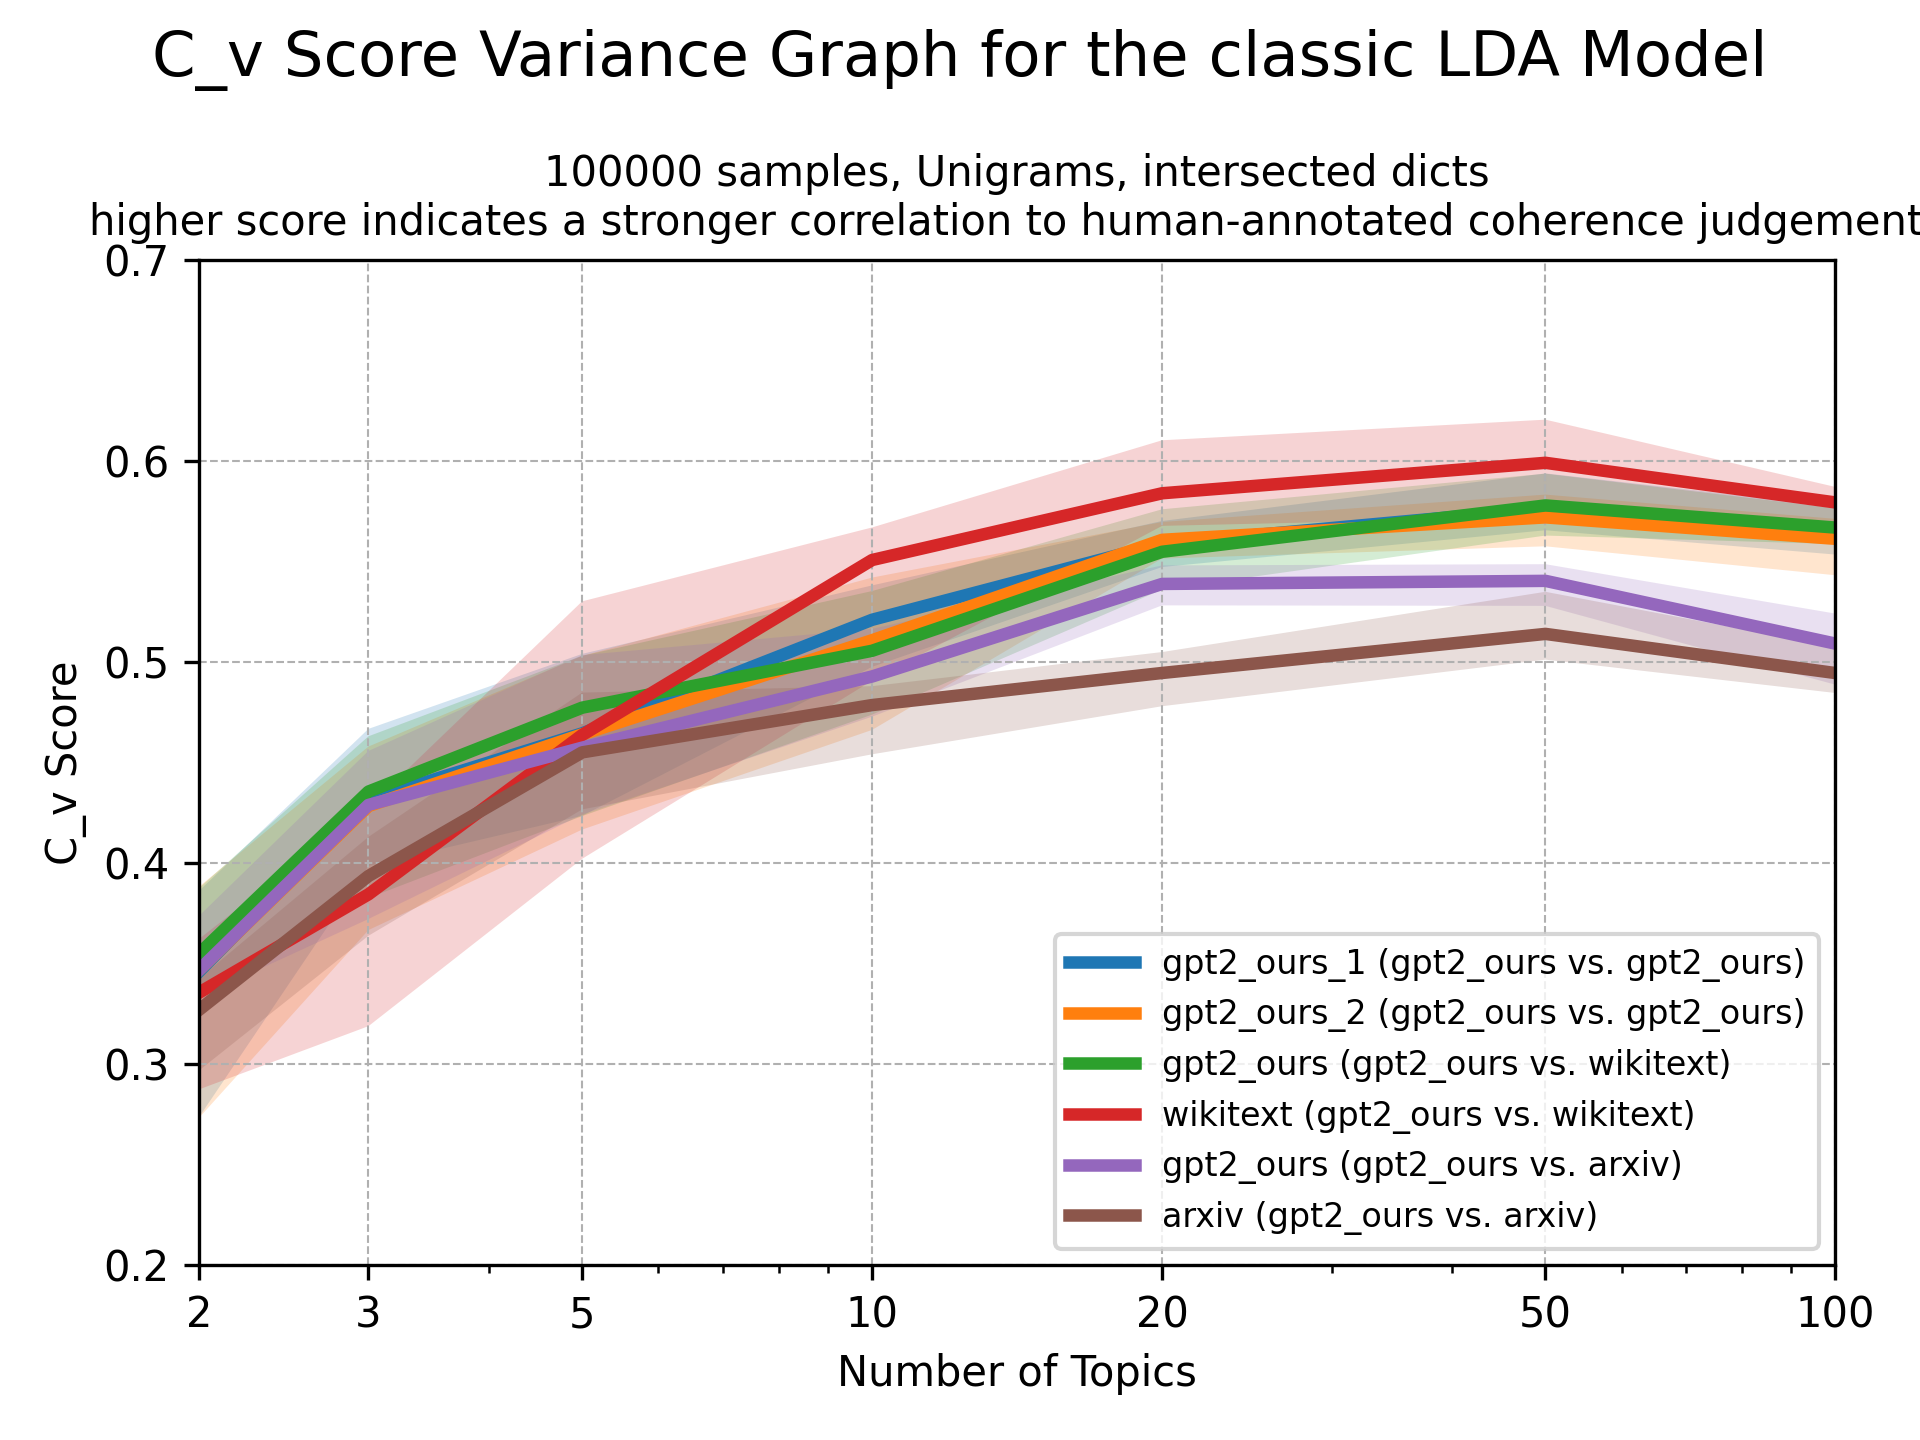
\includegraphics[width=0.6\textwidth]{figures/Unigrams-100000-var-cv-is}
    \caption{Topic coherence of topic models with different seed.}
    \label{fig:Unigrams-100000-var-cv-is}
\end{figure}
Secondly, we compare the influence of a slightly changed dictionary. As previously mentioned, we take the intersection of each dictionary pair of which we want to compare the corpora. This means, when looking at the \texttt{wikitext} corpus, we get 7 different dictionaries and therefore 7 slightly different topic models for that corpus. Those different dictionaries result from comparing the corpus with \texttt{gpt2}, \texttt{arxiv}, \texttt{gpt\_ours}, \texttt{gpt\_ours} with Top-P sampling, \texttt{gpt\_ours} with Typical sampling and twice for \texttt{wikitext} itself. As shown in fig. \ref{fig:Unigrams-100000-crossmodel-cv-var-classic_lda-gpt2+nt-is} on the left, the topic model scores are in a similar range of $0.29$ to $0.59$ with a variance of $\pm0.05$. On average, we can see that the quality of each of our topic models here is the highest when using $20$ to $50$ topics. 

We also evaluate the influence of different sampling methods for the \texttt{gpt2\_own} corpus and the quality of the resulting topic models. Fig. \ref{fig:Unigrams-100000-crossmodel-cv-var-classic_lda-gpt2+nt-is} on the right shows that on average Top-P and even more so Typical sampling improves the quality of topics created by topic models.
\begin{figure}[H]
    \centering
    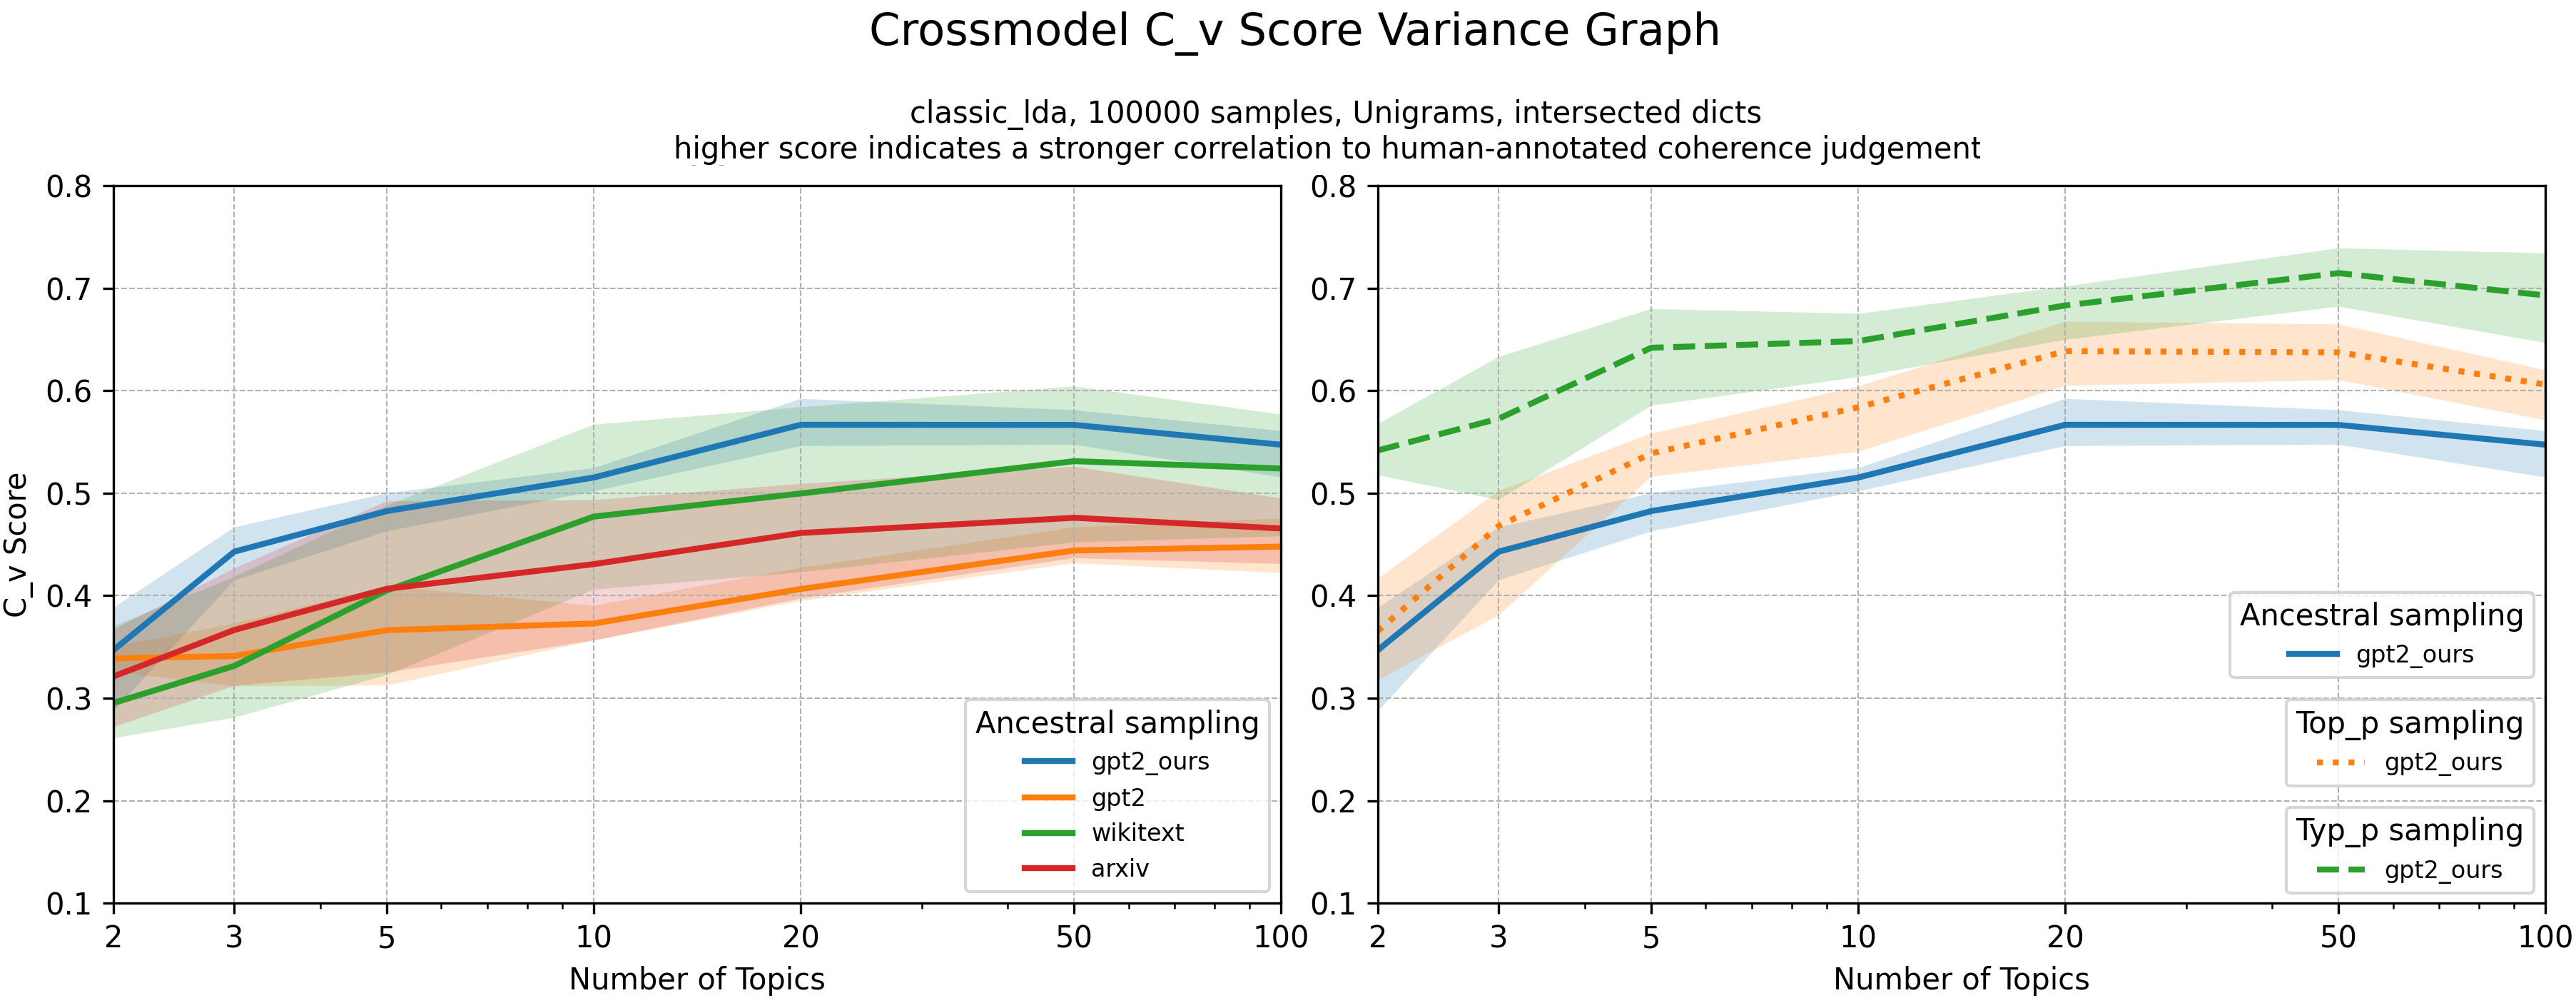
\includegraphics[width=1\textwidth]{figures/Unigrams-100000-crossmodel-cv-var-classic_lda-gpt2+nt-is}
    \caption{Topic coherence of topic models with slightly different dictionaries.}
    \label{fig:Unigrams-100000-crossmodel-cv-var-classic_lda-gpt2+nt-is}
\end{figure}

% =======================================
\subsubsection{Corpora With 10'000 Samples}
Similar to corpora with 100'000 documents, for corpora with 10'000 documents, we first compare the influence of changing the seed when creating a topic model. The mean and variance is taken from topic models with different seeds. In fig. \ref{fig:Unigrams-10000-var-cv-is}, the mean ranges from $0.31$ to $0.58$ and the variance stays in range of $\pm0.05$ of the mean. On average, we see that the quality of each of our topic models here is the highest when using $10$ to $50$ topics, depending on the corpus. 
\begin{figure}[H]
    \centering
    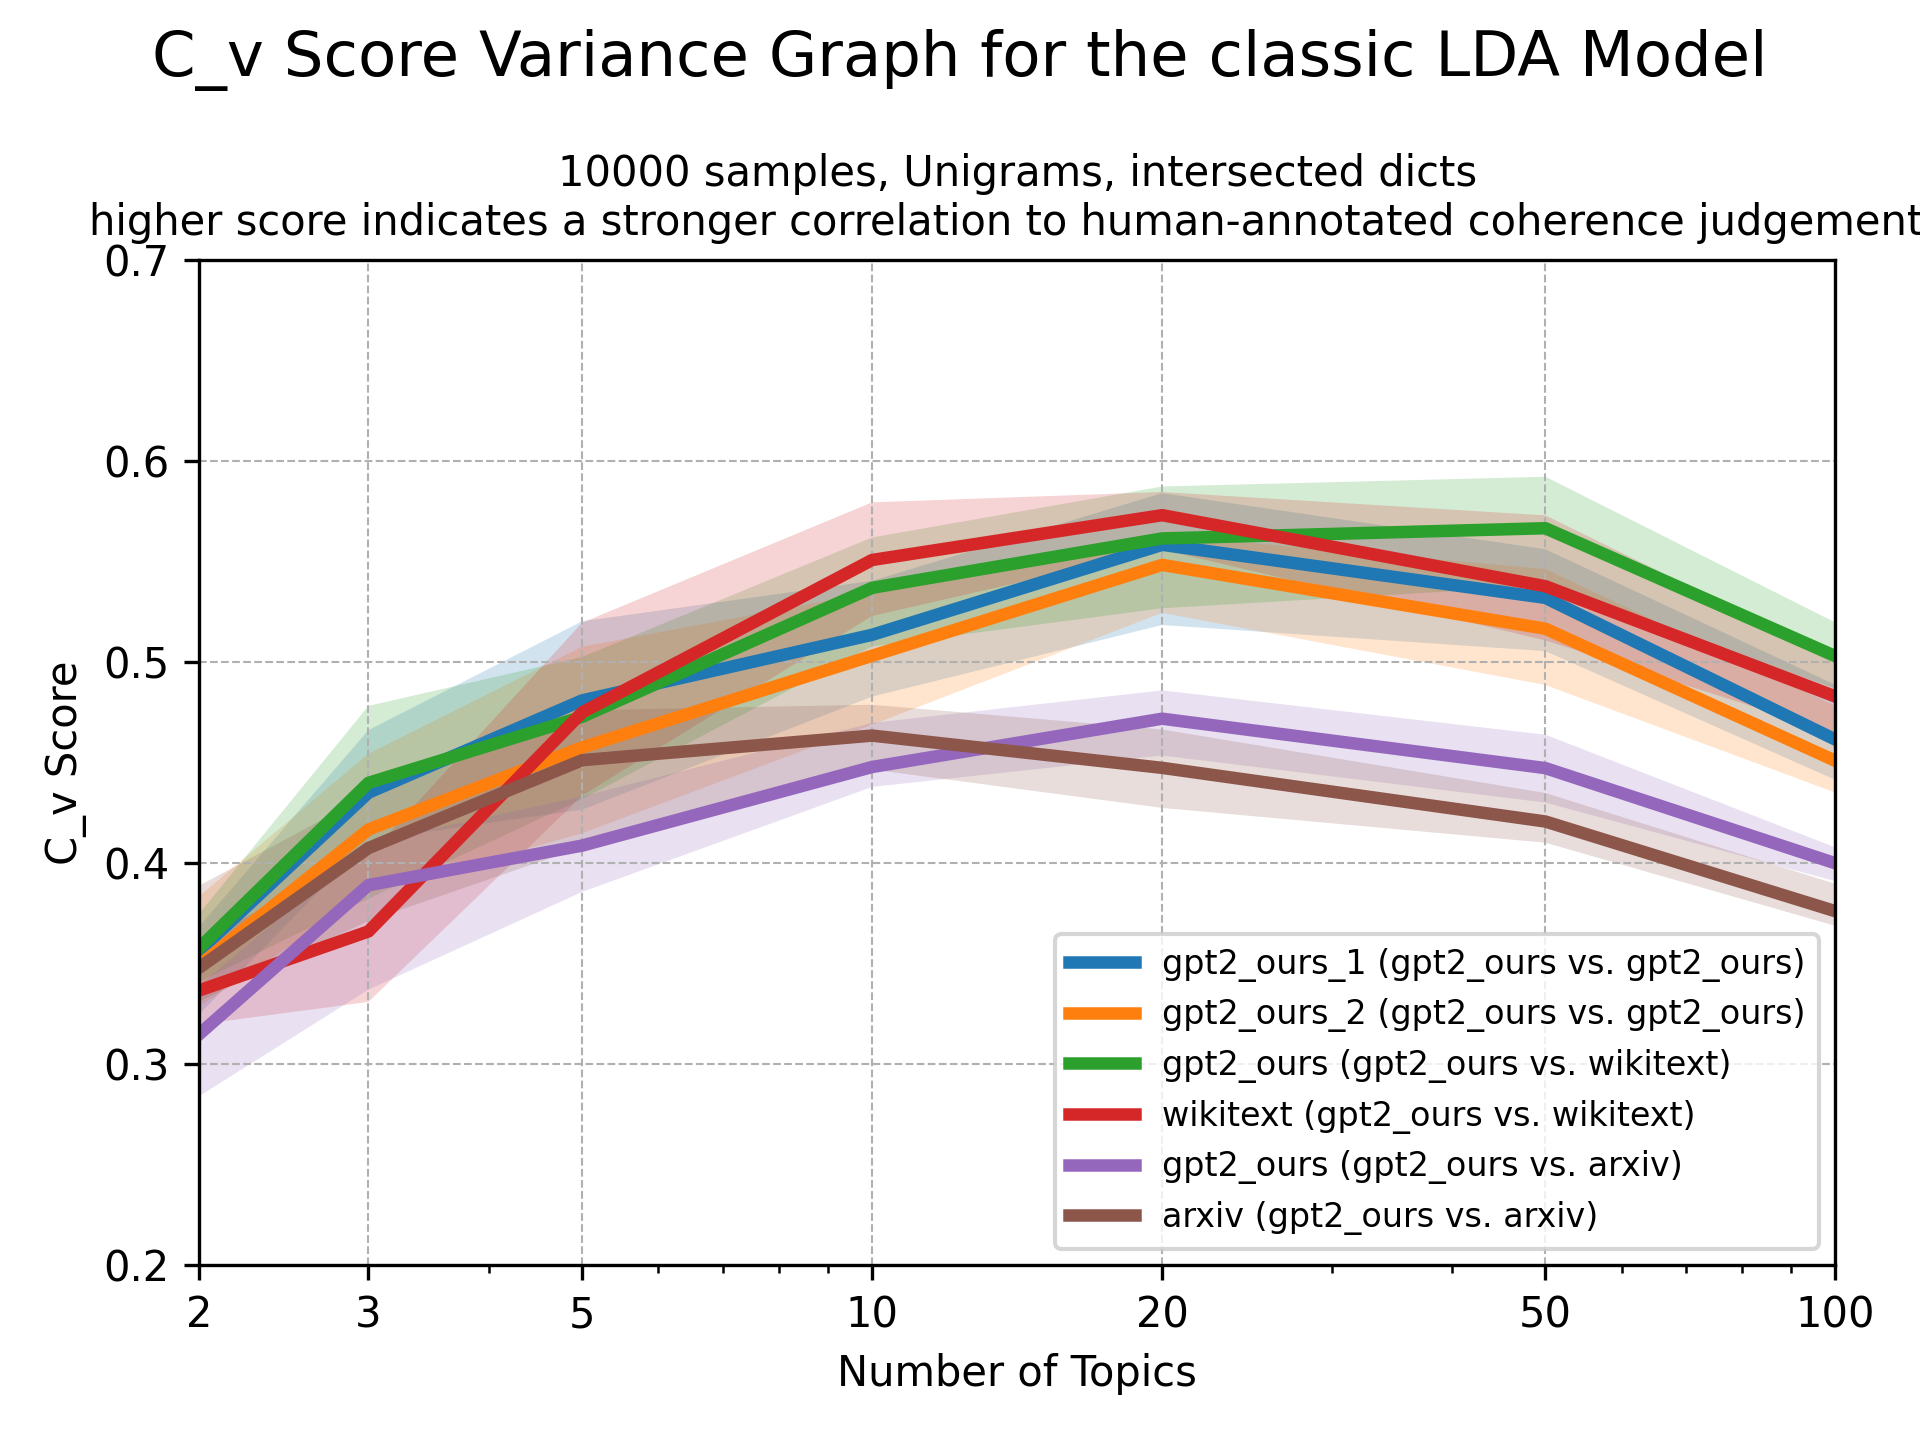
\includegraphics[width=0.6\textwidth]{figures/Unigrams-10000-var-cv-is}
    \caption{Topic coherence of topic models with changing seed.}
    \label{fig:Unigrams-10000-var-cv-is}
\end{figure}
We also compare the effect of a slightly changed dictionary. In contrast to 100'000 samples, we now have additional topic models. We add the evaluation of topic models created with the neural LDA and from additional corpora, i.e. \texttt{trafo\_xl}, \texttt{trafo\_xl\_own}, \texttt{trafo\_xl\_own} sampled with Top-P sampling and \texttt{trafo\_xl\_own} sampled with Typical sampling. With this, we get 11 topic models for the \texttt{wikitext} corpus with a (slightly) different dictionary. 

% =======================================
\subsubsection{GPT-2 With Classic LDA}
Fig. \ref{fig:Unigrams-10000-crossmodel-cv-var-classic_lda-gpt2+nt-is} on the left shows the results in respect to the GPT-2 models. The topic model scores are in a range of $0.31$ to $0.53$ with a variance of $\pm0.05$. On average, we can see that the quality of each of our topic models here is the highest when using $5$ to $20$ topics, depending on the corpus.

Fig. \ref{fig:Unigrams-10000-crossmodel-cv-var-classic_lda-gpt2+nt-is} on the right shows the influence of different sampling methods for the \texttt{gpt2\_own} corpus. On average, Top-P and even more Typical sampling improve the quality of topics created by topic models.
\begin{figure}[H]
    \centering
    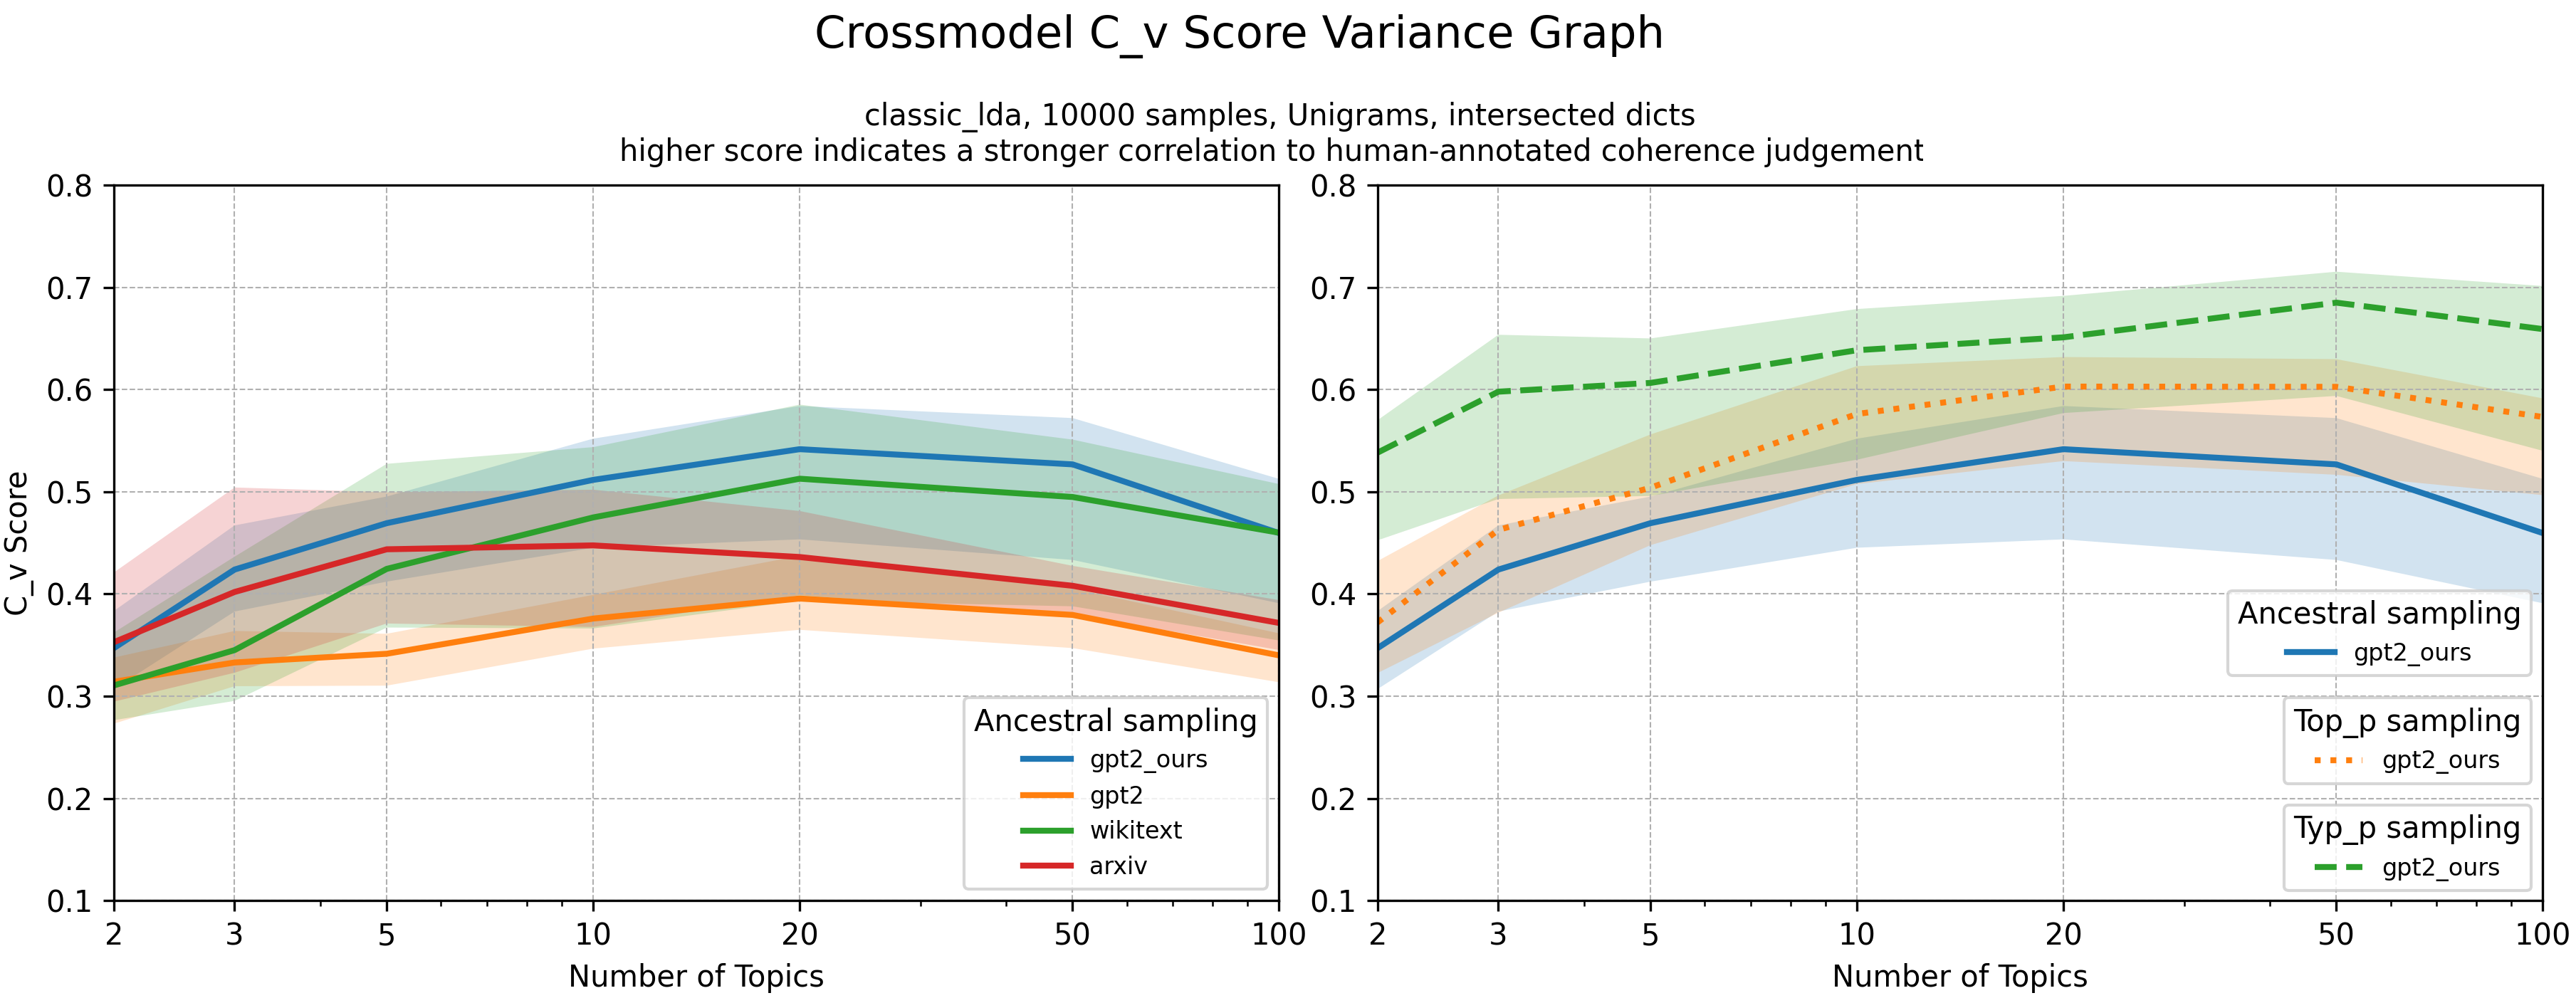
\includegraphics[width=1\textwidth]{figures/Unigrams-10000-crossmodel-cv-var-classic_lda-gpt2+nt-is}
    \caption{Topic coherence of topic models with slightly different dictionaries.}
    \label{fig:Unigrams-10000-crossmodel-cv-var-classic_lda-gpt2+nt-is}
\end{figure}

% =======================================
\subsubsection{Transformer-XL With Classic LDA}
Fig. \ref{fig:Unigrams-10000-crossmodel-cv-var-classic_lda-trafo_xl+nt-is} on the left shows our results with classic LDA in reference to the Tranformer-XL models. The topic model scores are in a range of $0.31$ to $0.56$ with a variance of $\pm0.1$. On average, we see that the quality of our topic models is the highest when using $5$ to $20$ topics, depending on the corpus.

In fig. \ref{fig:Unigrams-10000-crossmodel-cv-var-classic_lda-trafo_xl+nt-is} on the right, we see that for a lower number of topics (2 to 10), different sampling methods do not make a notable difference. For topic models with a topic count of 10 or more Top-P and even more Typical sampling leads to better topic models than ancestral sampling.
\begin{figure}[H]
    \centering
    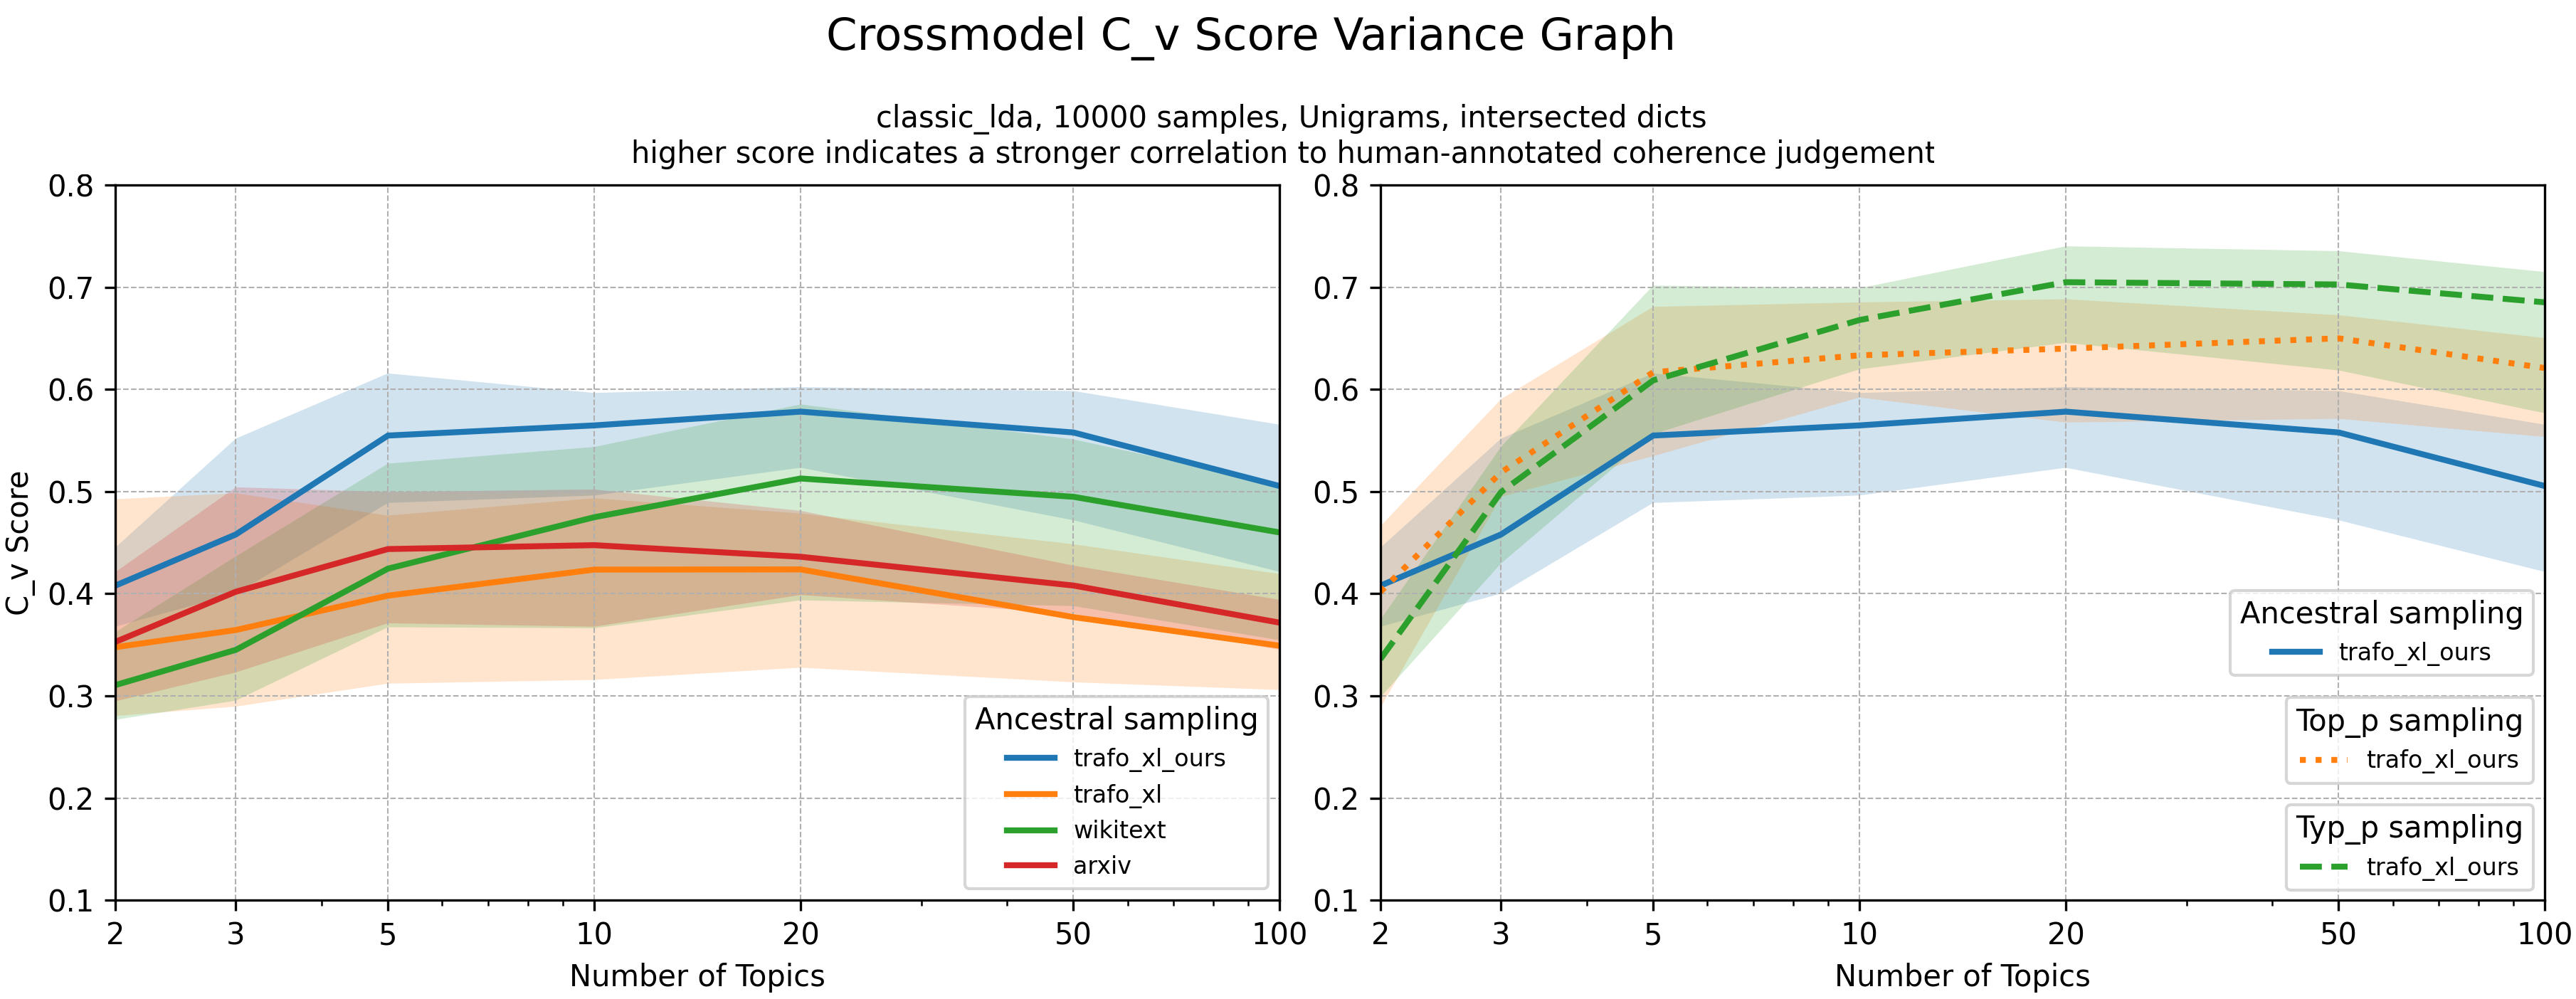
\includegraphics[width=1\textwidth]{figures/Unigrams-10000-crossmodel-cv-var-classic_lda-trafo_xl+nt-is}
    \caption{Topic coherence of topic models with slightly different dictionaries.}
    \label{fig:Unigrams-10000-crossmodel-cv-var-classic_lda-trafo_xl+nt-is}
\end{figure}

% =======================================
\subsubsection{GPT-2 With Neural LDA}
Fig. \ref{fig:Unigrams-10000-crossmodel-cv-var-neural_lda-gpt2+nt-is} shows the quality of topic models created with neural LDA in respect to GPT-2 models. Interestingly, the inverse peak is at 3 topics. All topic models created with neural LDA have this in common. After 5 topics, the scores range from $0.3$ to $0.45$ with a variance of up to $\pm0.1$. The quality with 5 topics or more is approximately horizontal and definitely worse than with the classic LDA. 

The influence of different sampling methods for the \texttt{gpt2\_own} corpus and the quality of the resulting topic models is shown in fig. \ref{fig:Unigrams-10000-crossmodel-cv-var-neural_lda-gpt2+nt-is}. Note that by changing the sampling method, the inverse peak observed with ancestral sampling at 3 topics gets smoothed out. On average, Top-P and even more Typical sampling improve the quality of topics created by topic models.
\begin{figure}[H]
    \centering
    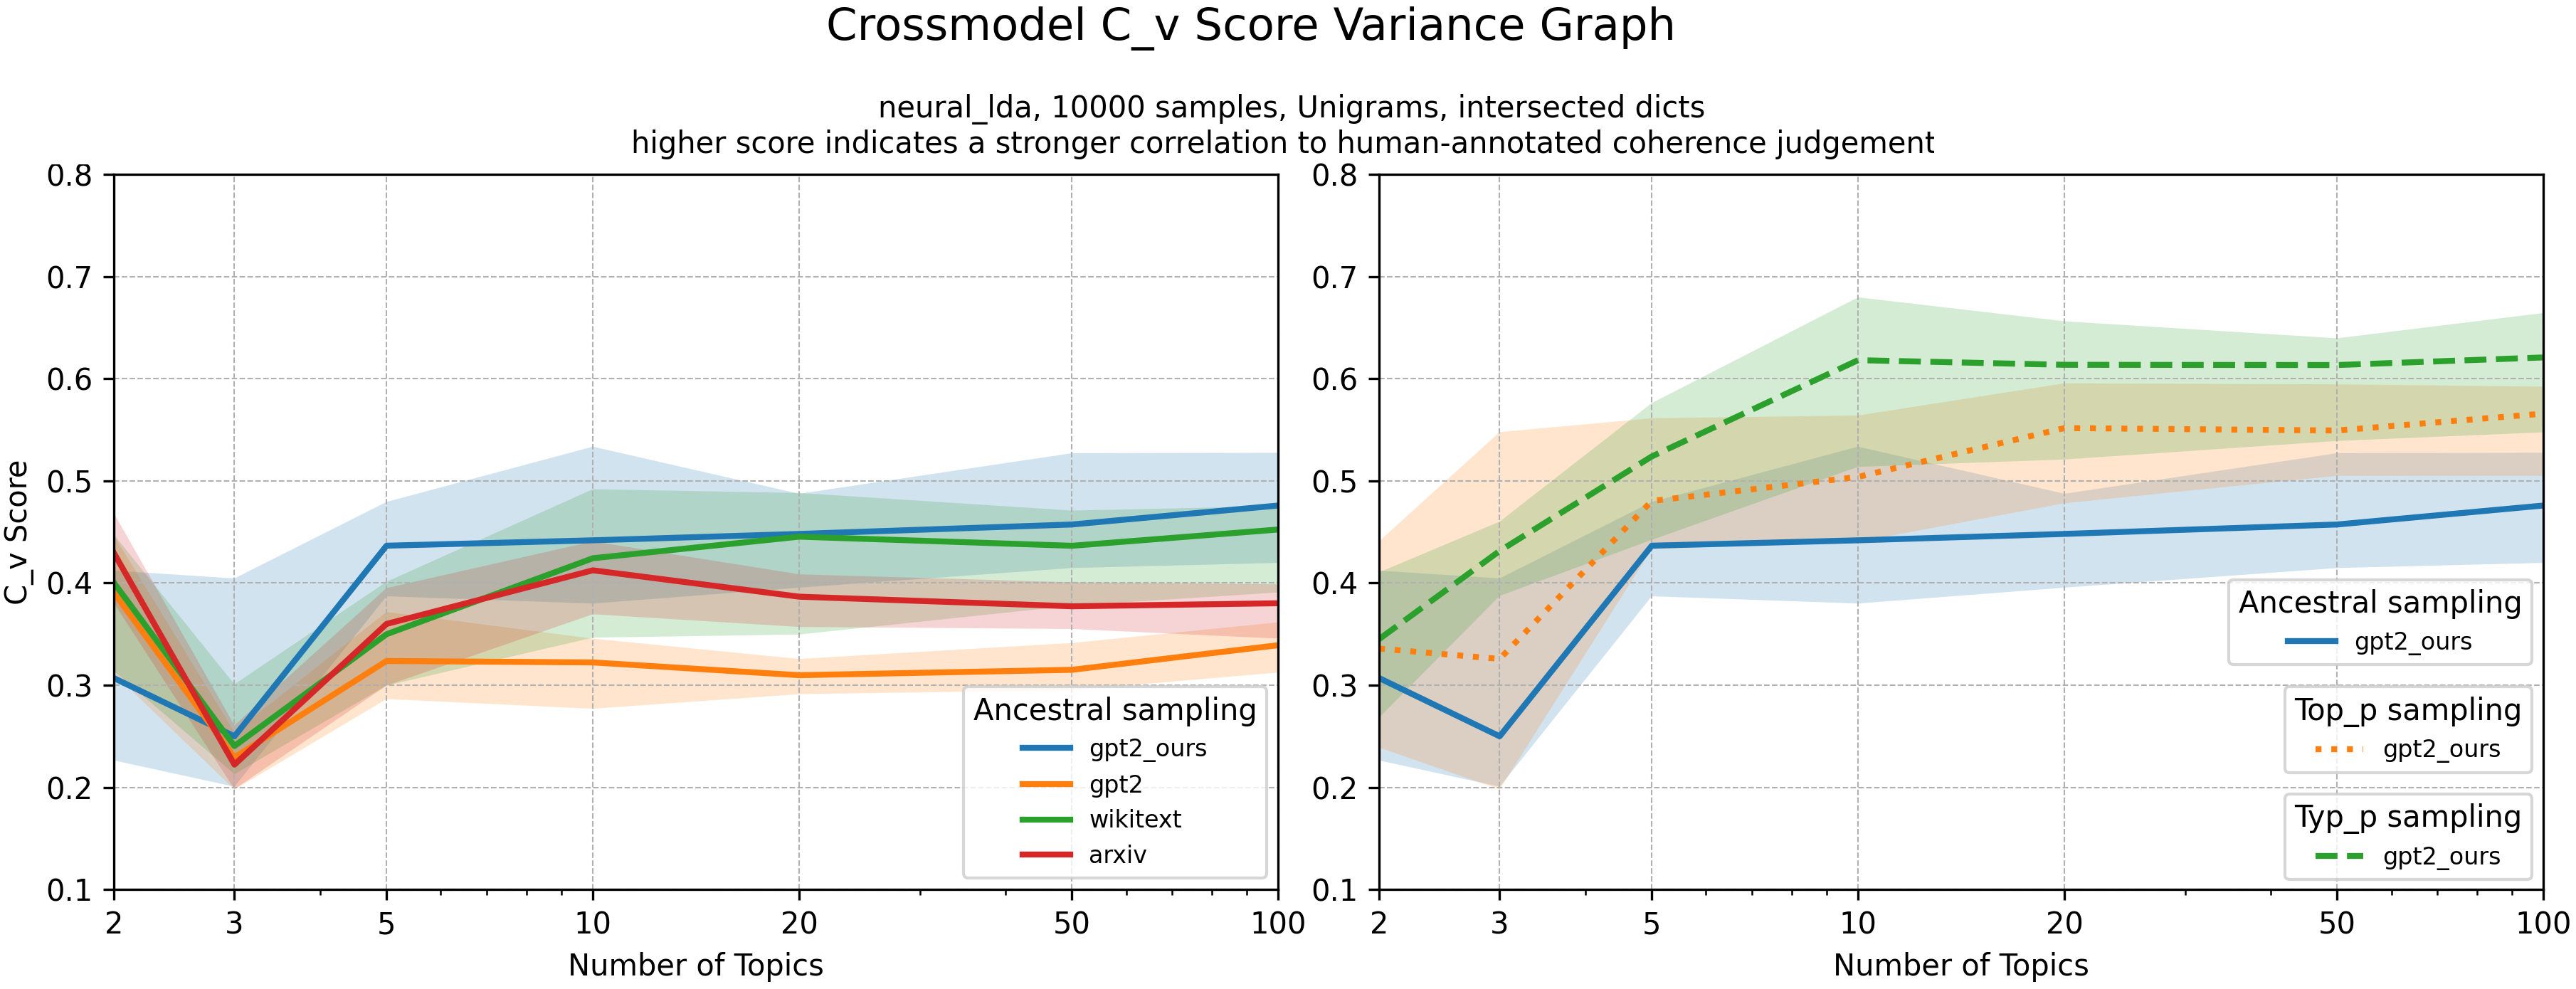
\includegraphics[width=1\textwidth]{figures/Unigrams-10000-crossmodel-cv-var-neural_lda-gpt2+nt-is}
    \caption{Topic coherence of topic models with slightly different dictionaries.}
    \label{fig:Unigrams-10000-crossmodel-cv-var-neural_lda-gpt2+nt-is}
\end{figure}

% =======================================
\subsubsection{Transformer-XL With Neural LDA}
The quality of topic models created with neural LDA in respect to both Transformer-XL models is very similar to the GPT-2 results. In fig. \ref{fig:Unigrams-10000-crossmodel-cv-var-neural_lda-trafo_xl+nt-is} on the left, we see again the peaks at 3 topics. At a topic size of 5 or more, the topic model quality ranges from $0.31$ to $0.51$ with a variance of up to $\pm0.1$. The quality of 5 topics or more is more or less horizontal and on average worse than the classic LDA topic models. 

The quality of neural LDA topic models from the corpus sampled with Typical (and Top-P) sampling is much smoother. Additionally, for 3 topics or more, the quality is improved (see fig. \ref{fig:Unigrams-10000-crossmodel-cv-var-neural_lda-trafo_xl+nt-is} on the right).
\begin{figure}[H]
    \centering
    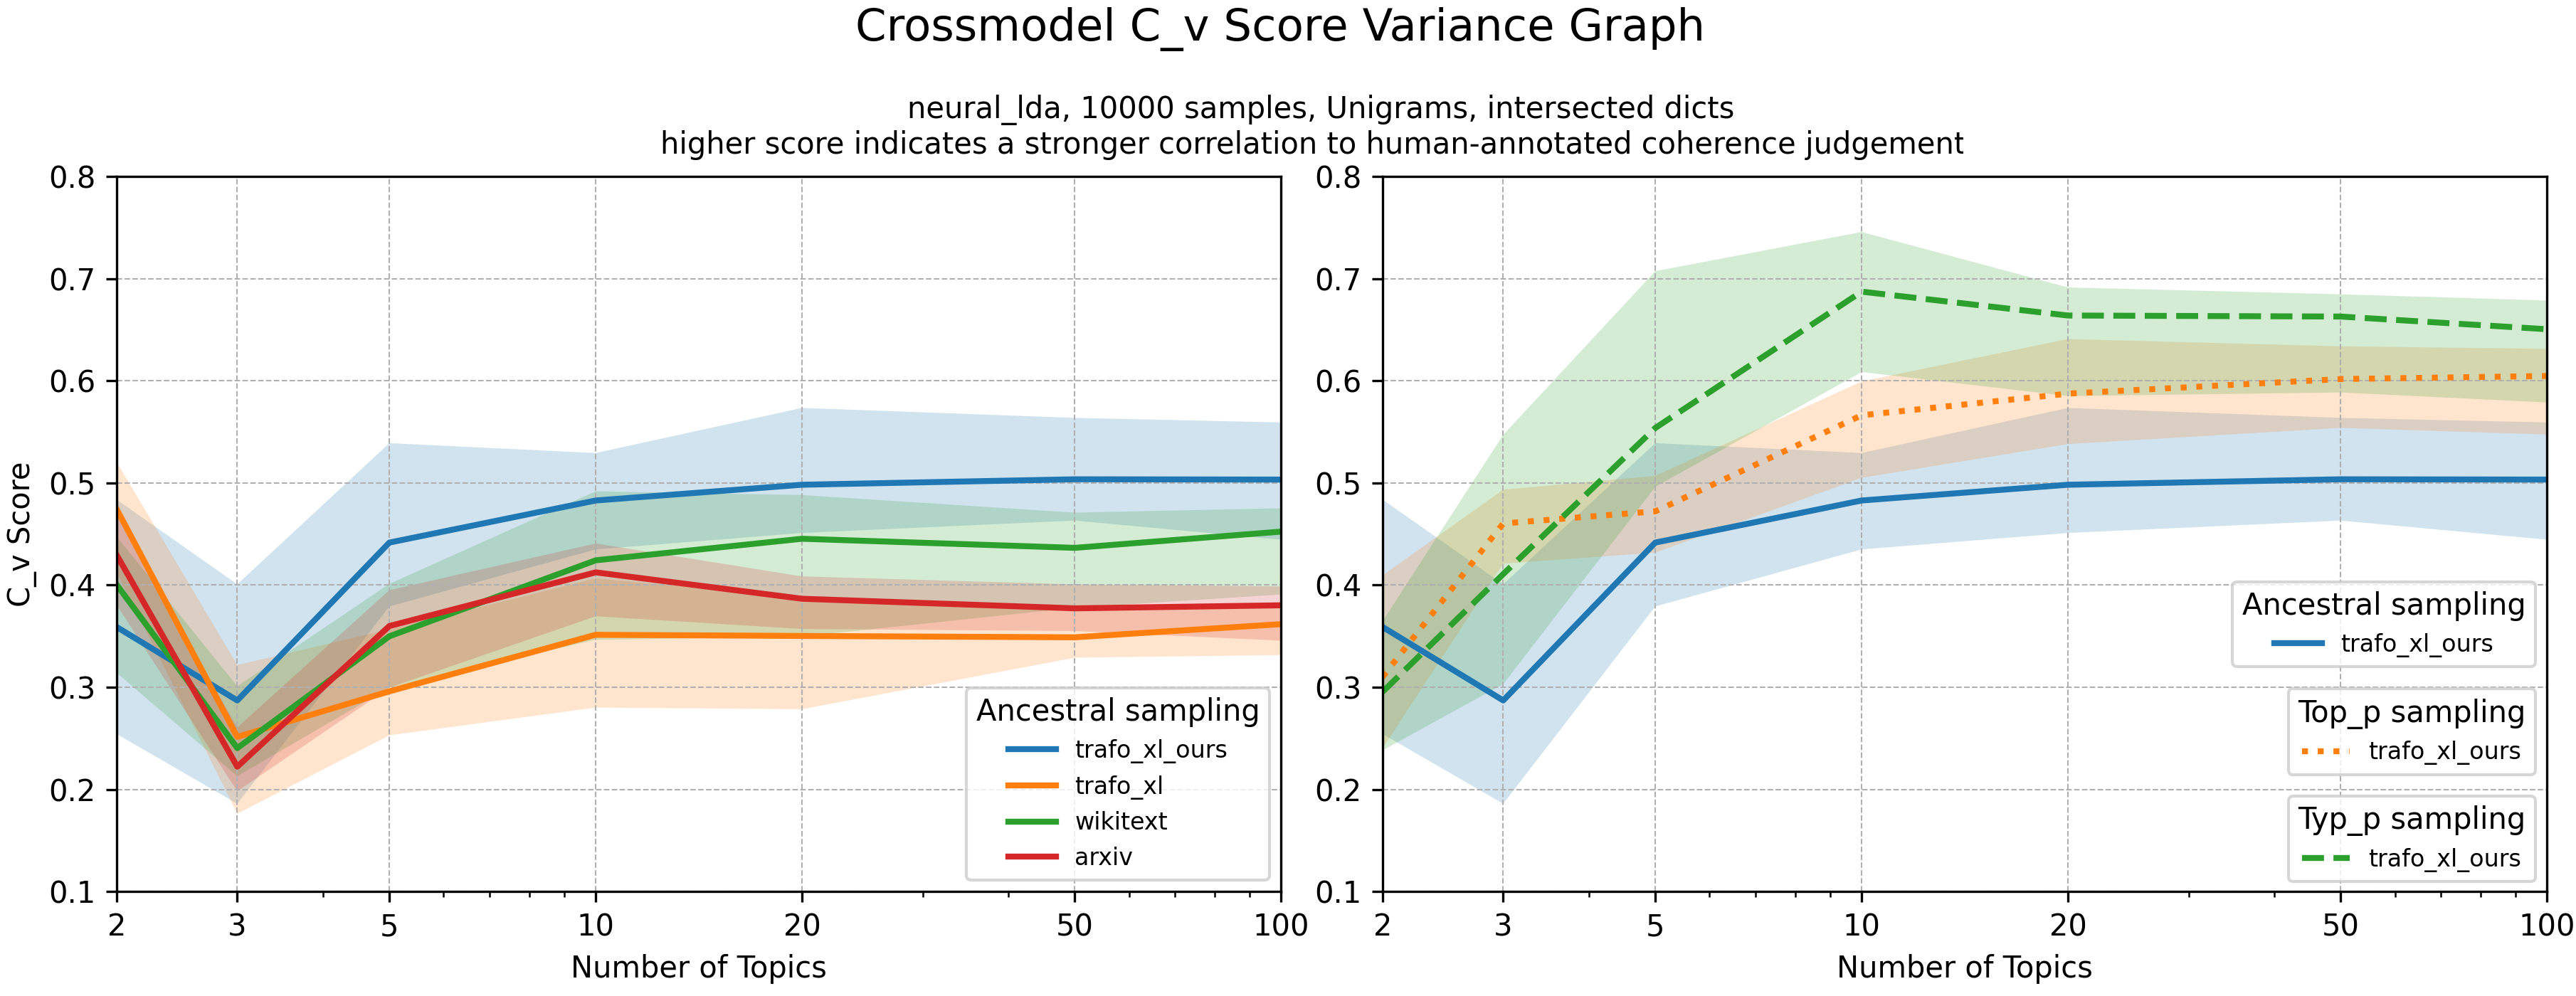
\includegraphics[width=1\textwidth]{figures/Unigrams-10000-crossmodel-cv-var-neural_lda-trafo_xl+nt-is}
    \caption{Topic coherence of topic models with slightly different dictionaries.}
    \label{fig:Unigrams-10000-crossmodel-cv-var-neural_lda-trafo_xl+nt-is}
\end{figure}


% =======================================
\subsection{Variance of Our Metric for Comparing Topic Models}
To be able to make some assumptions about our final results with a certain degree of confidence, we measure the variance of our metric on the following topic model comparisons for 100'000 and 10'000 documents: \texttt{gpt2\_ours} vs. \texttt{gpt2\_ours}, \texttt{gpt2\_ours} vs. \texttt{wikitext} and \texttt{gpt2\_ours} vs. \texttt{arxiv}.

Fig. \ref{fig:Unigrams-var-tt-is} shows that for topic models with a higher number of topics, especially for corpora with 100'000 documents (graph on the left), the metric tends to be stable in respect to variance. The variance for topic models from corpora with 100'000 documents collapses nearly to 0 for a higher number of topics. Topic models from corpora with 10'000 documents tend to have a slightly higher variance of up to $\pm0.1$.  
\begin{figure}[H]
    \centering
    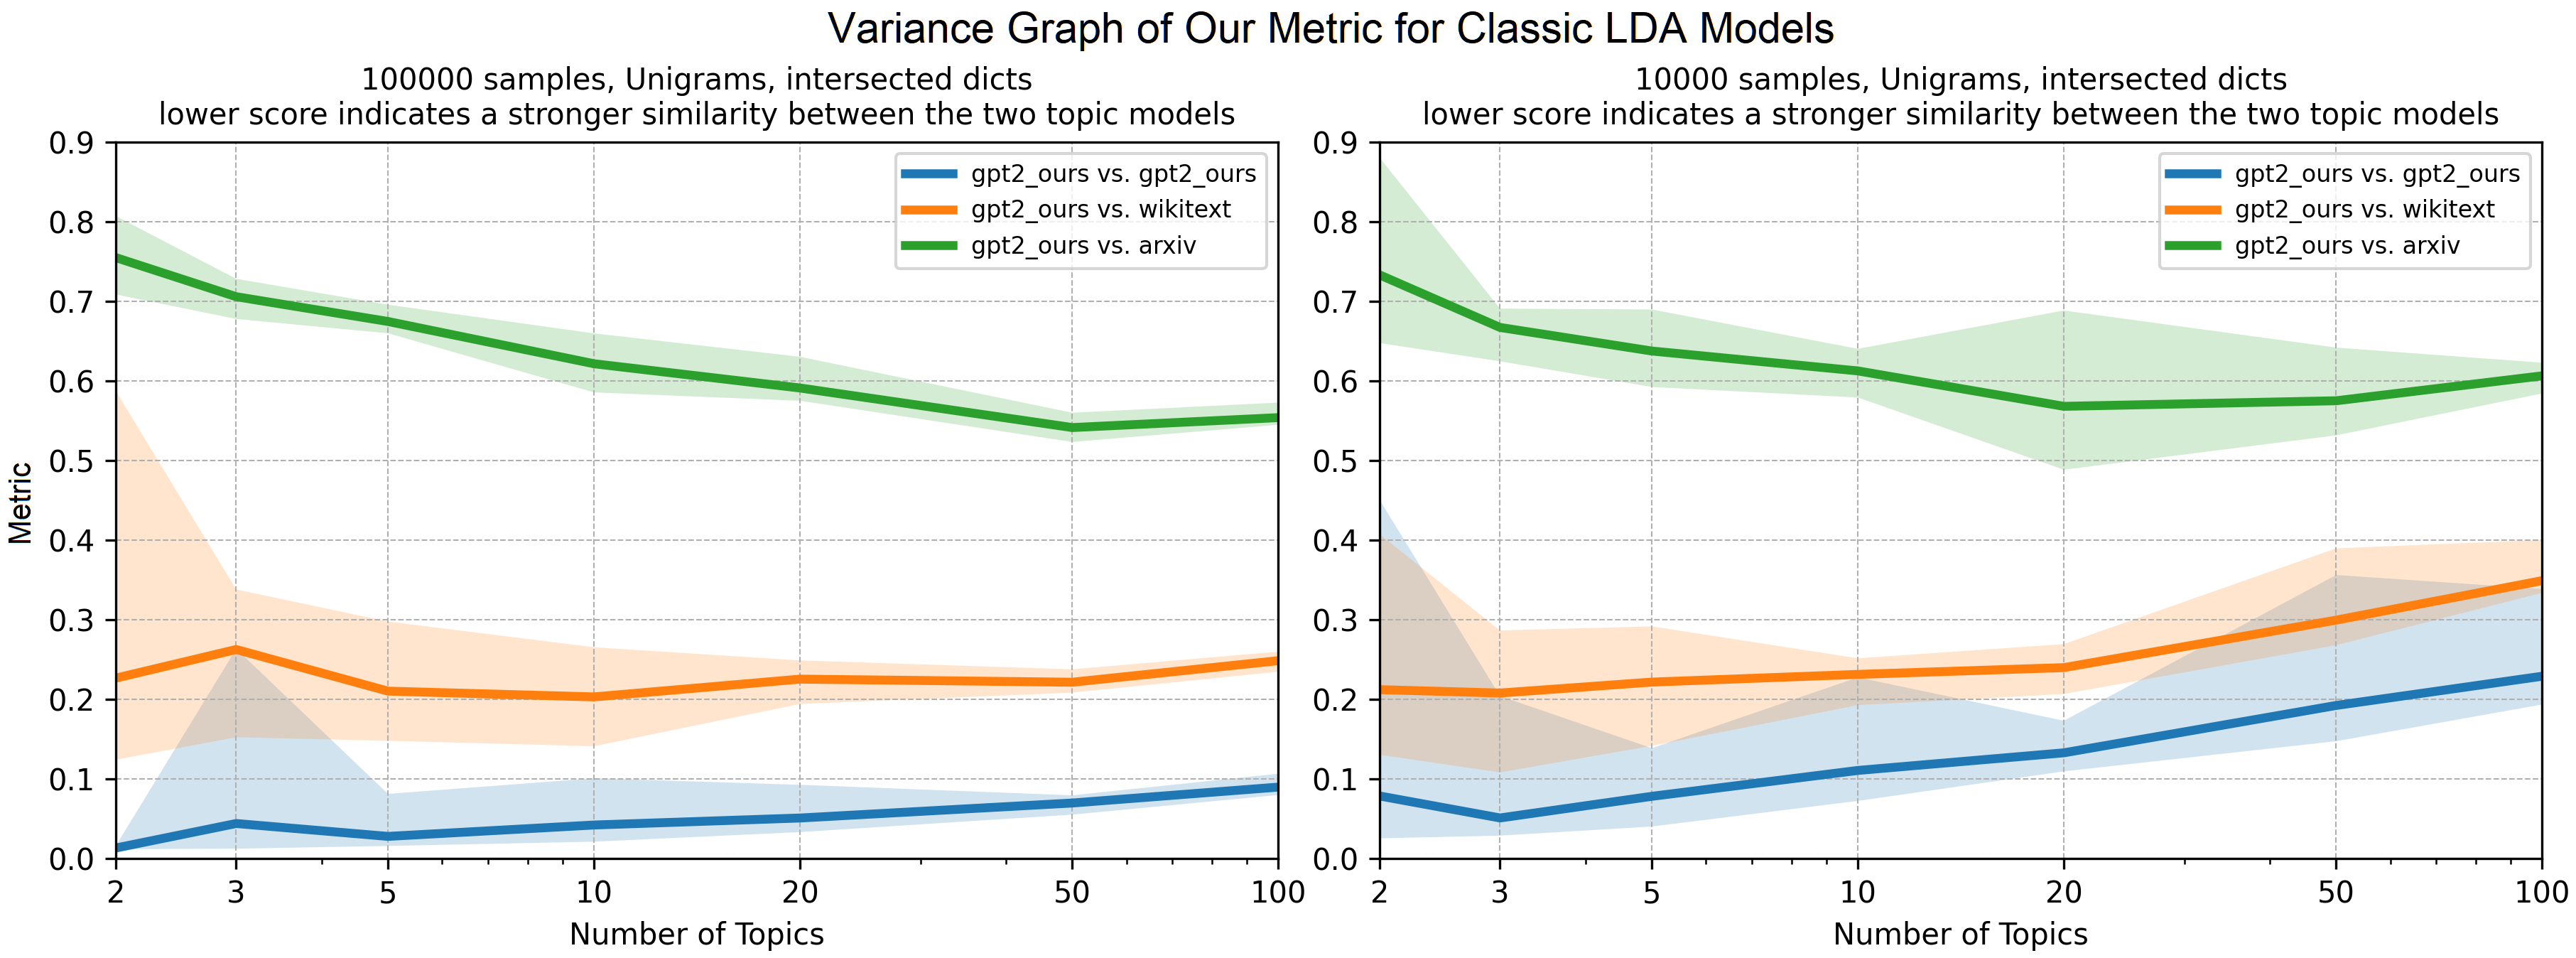
\includegraphics[width=1\textwidth]{figures/Unigrams-var-tt-is}
    \caption{Variance of the topic model comparison metric for corpora with 100'000 and 10'000 samples.}
    \label{fig:Unigrams-var-tt-is}
\end{figure}

% =======================================
\subsection{Comparisons of Our Topic Models}\label{sec:comp}
In order to make some assumptions about our findings, we need a baseline. Specifically, we need to know what it means to compare two similar topic models and what it means to compare two dissimilar topic models in respect to our metric. 

To find an upper boundary for the area of similar topic models, we compare topic models from the same corpus, i.e. \texttt{dataset1-*} vs. \texttt{dataset2-*}. To find a lower boundary for the area of different topic models, we compare topic models from corpora we know are different, i.e. \texttt{wikitext} vs. \texttt{arxiv}.

% =======================================
\subsubsection{Corpora With 100'000 Documents}
For corpora with 100'000 documents (see fig. \ref{fig:Unigrams-100000-crossmodel-tt-gpt2-classic_lda-ab-is} on the left), the \texttt{arxiv} corpus compared to other corpora results in a value of greater than $0.52$. When comparing topic models from the same corpora, the value is below $0.2$. The comparisons between topic models from corpora \texttt{gpt2\_ours}, \texttt{gp2} and \texttt{wikitext} result in a value ranging from $0.2$ and $0.52$.

In contrast to the improvement in quality of our topic models with help of other sampling methods, we cannot say the same in regard to our comparison metric. In fig. \ref{fig:Unigrams-100000-crossmodel-tt-gpt2-classic_lda-ab-is} on the right, we cannot see a general improvement of our metric values when using Typical or Top-P sampling. Instead, in some occasions (dashed red line vs. red line), the topic models differ clearly from each other. 
\begin{figure}[H]
    \centering
    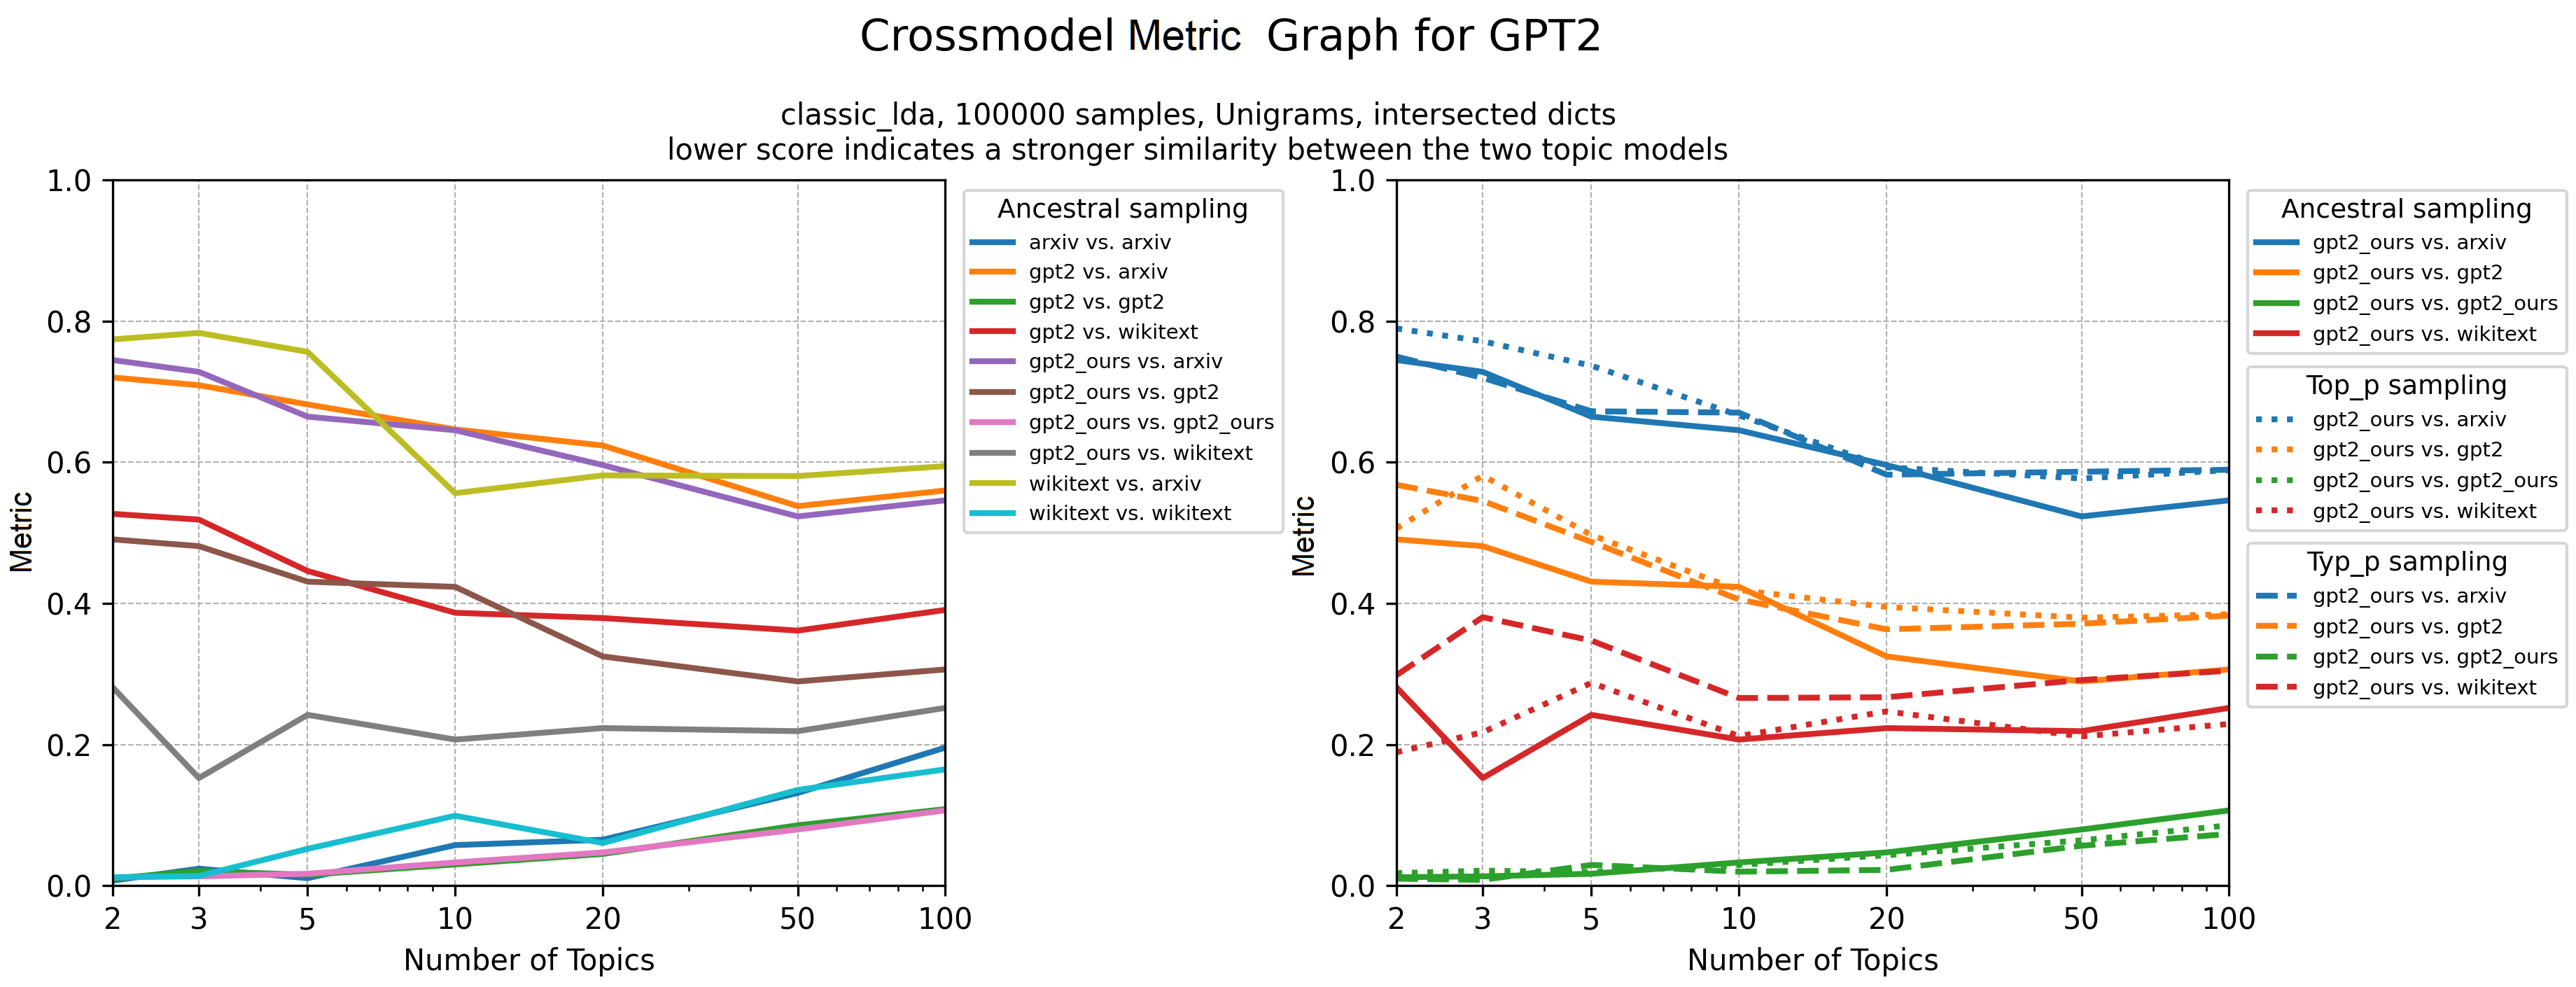
\includegraphics[width=1\textwidth]{figures/Unigrams-100000-crossmodel-tt-gpt2-classic_lda-ab-is}
    \caption{Topic model comparison metric (GPT-2, classic LDA, 100'000 samples).}
    \label{fig:Unigrams-100000-crossmodel-tt-gpt2-classic_lda-ab-is}
\end{figure}

% =======================================
\subsubsection{Corpora With 10'000 Documents}
% =======================================
\subsubsection{GPT-2 and Classic LDA}
For corpora with 10'000 documents in respect to GPT-2 and topic models created with classic LDA (see fig. \ref{fig:Unigrams-10000-crossmodel-tt-gpt2-classic_lda-ab-is} on the left), the \texttt{arxiv} corpus compared to other corpora results in a value of greater than $0.5$. When comparing topic models from the same corpora, the value is below $0.2$. For topic sizes of up to 20 topics, the value is below $0.4$. The comparisons between topic models from corpora \texttt{gpt2\_ours} and \texttt{wikitext} result in a value ranging from $0.14$ to $0.32$.

In contrast to the topic model quality measurements, other sampling methods do not seem to improve our comparison metric. In fig. \ref{fig:Unigrams-10000-crossmodel-tt-gpt2-classic_lda-ab-is} on the right, we cannot see a general improvement of our values when using Typical or Top-P sampling. Instead, in some occasions (dashed red line vs. red line), the topic models differ clearly from each other.
\begin{figure}[H]
    \centering
    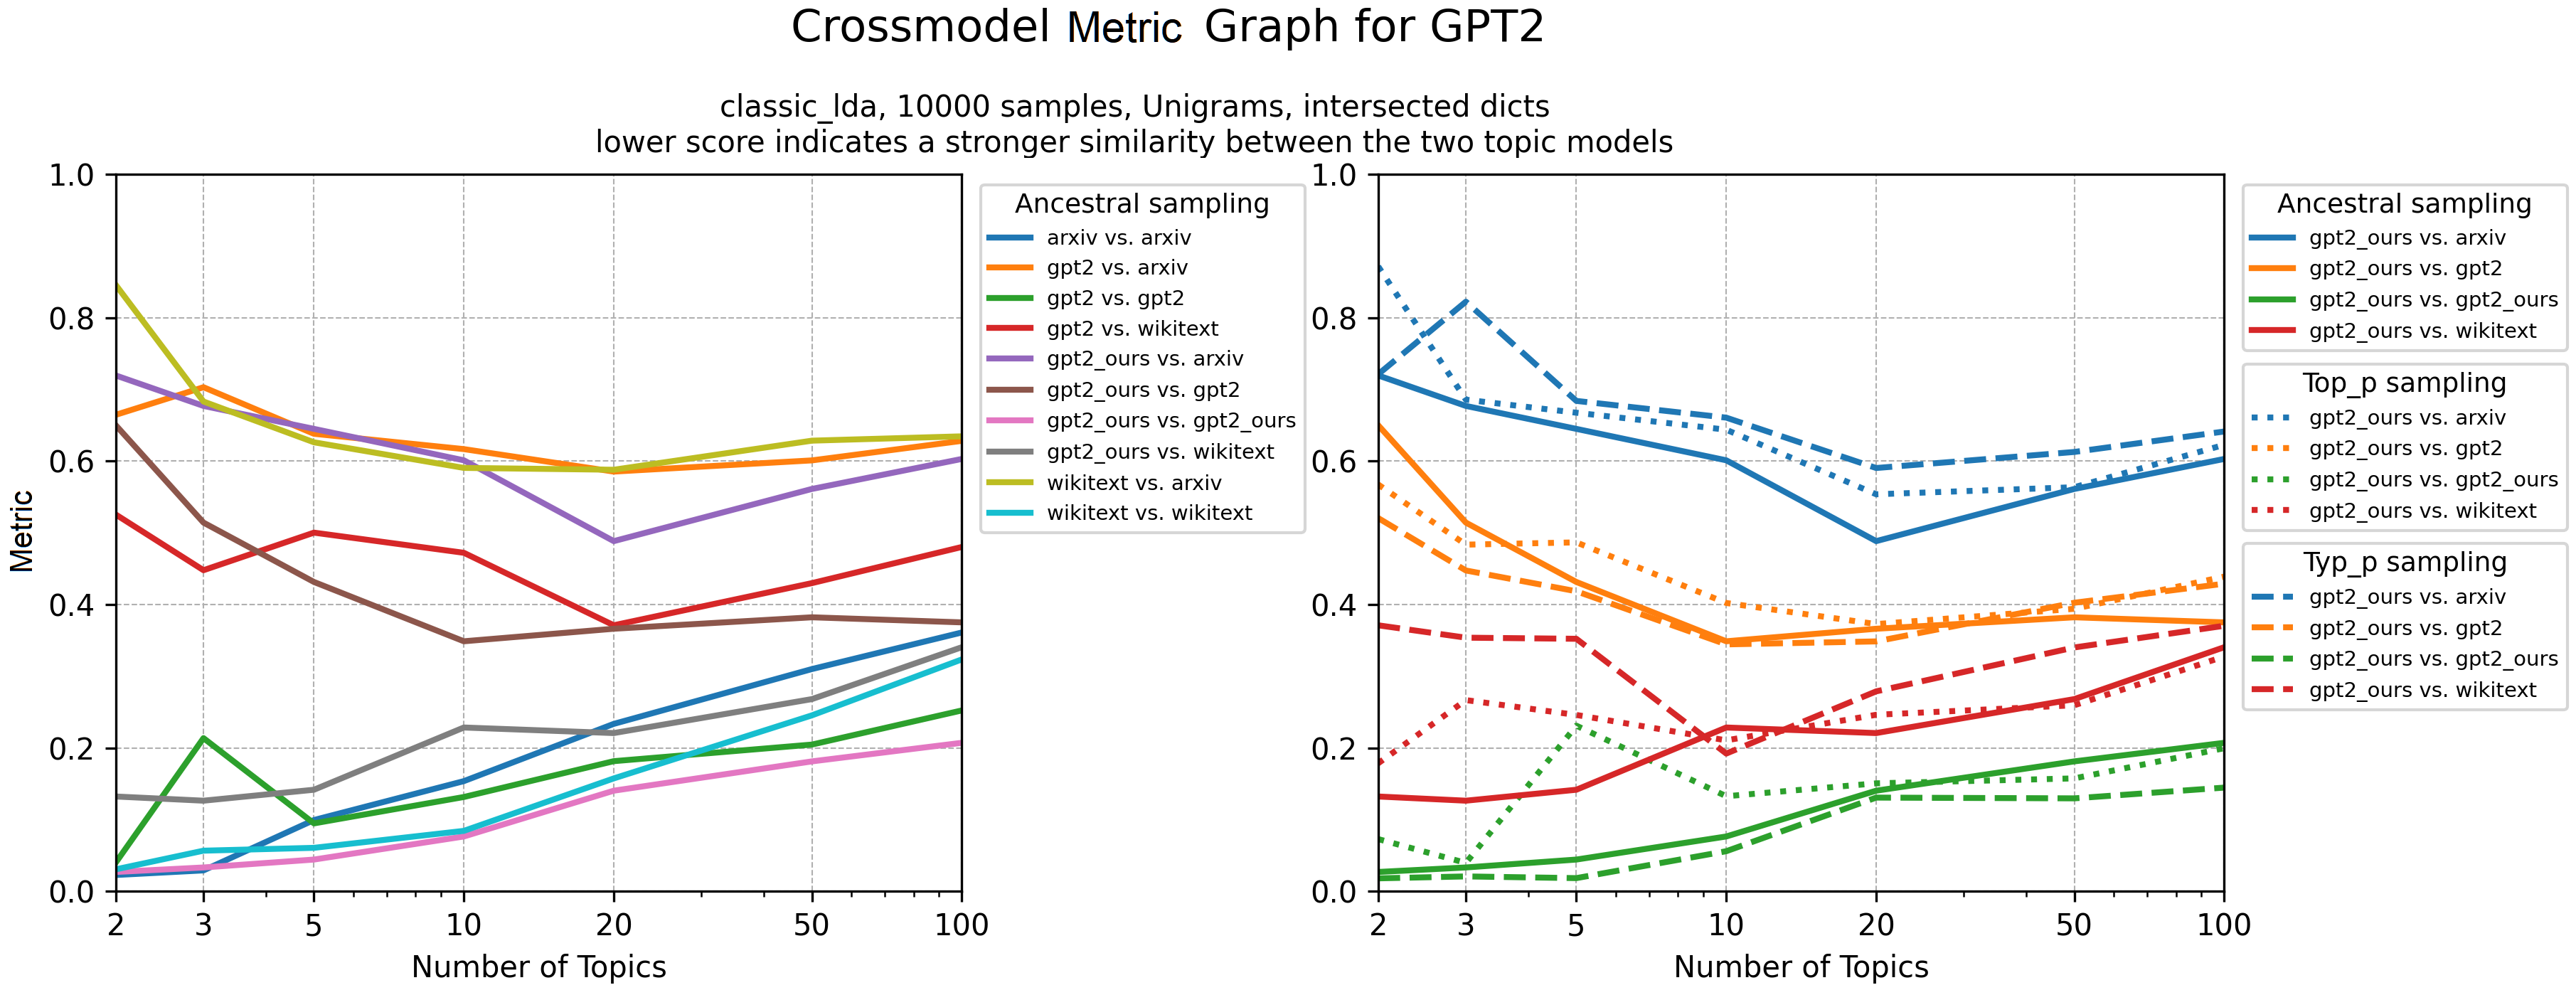
\includegraphics[width=1\textwidth]{figures/Unigrams-10000-crossmodel-tt-gpt2-classic_lda-ab-is}
    \caption{Topic model comparison score (GPT-2, classic LDA, 10'000 samples).}
    \label{fig:Unigrams-10000-crossmodel-tt-gpt2-classic_lda-ab-is}
\end{figure}

% =======================================
\subsubsection{Transformer-XL and Classic LDA}
For the results in respect to Transformer-XL and topic models created with classic LDA (see fig. \ref{fig:Unigrams-10000-crossmodel-tt-trafo_xl-classic_lda-ab-is} on the left), the \texttt{arxiv} corpus compared to other corpora results in a value above $0.6$. When comparing topic models from the same corpora, the upper boundary is linearly increasing from $0.2$ for topic size 2 up to $0.45$ for topic size 100. The comparisons between topic models from corpora \texttt{trafo\_xl\_ours} and \texttt{wikitext} result in a value slightly lower than the upper boundary from the area of similarity.

Other sampling methods have various impacts on our results. In fig. \ref{fig:Unigrams-10000-crossmodel-tt-trafo_xl-classic_lda-ab-is} on the right, we can see an improvement when comparing two nearly identical topic models (green line vs. green dashed/dotted line). For all other comparisons, there is no general improvement when using Typical or Top-P sampling.
\begin{figure}[H]
    \centering
    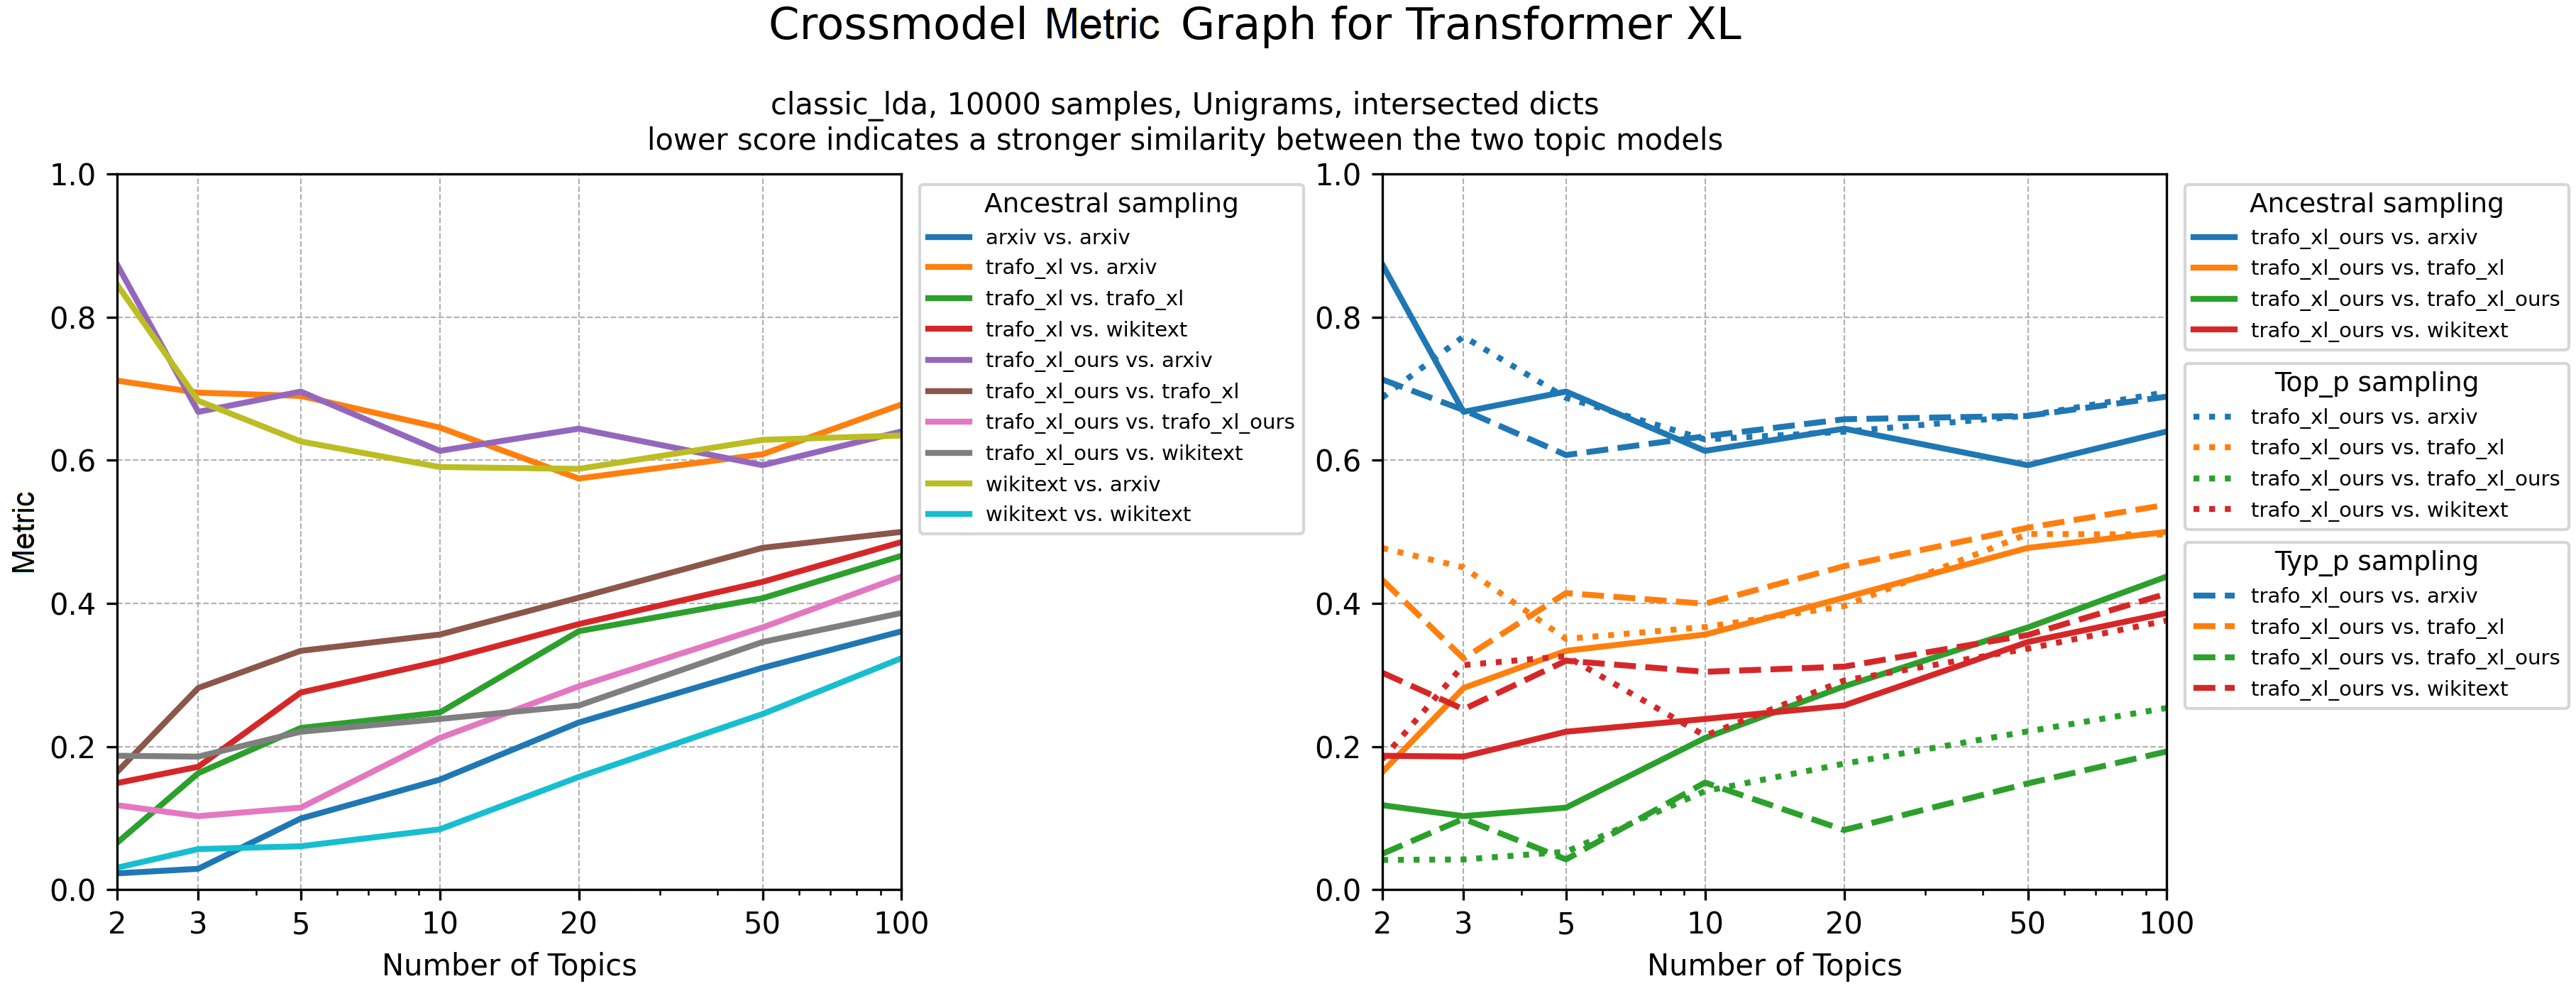
\includegraphics[width=1\textwidth]{figures/Unigrams-10000-crossmodel-tt-trafo_xl-classic_lda-ab-is}
    \caption{Topic model comparison metric (Transformer-XL, classic LDA, 10'000 samples).}
    \label{fig:Unigrams-10000-crossmodel-tt-trafo_xl-classic_lda-ab-is}
\end{figure}

% =======================================
\subsubsection{GPT-2 and Neural LDA}
In the results for GPT-2 and topic models created with neural LDA (see \ref{fig:Unigrams-10000-crossmodel-tt-gpt2-neural_lda-ab-is} on the left), we find some similar tendencies as in the data from before. The \texttt{arxiv} corpus compared to other corpora results in a value above $0.53$. When comparing topic models from the same corpora, the upper boundary is generally increasing from $0.1$ for a topic size of 2 up to $0.45$ for a topic size of 100. The results of the comparisons between topic models from corpora \texttt{gpt2\_ours} and \texttt{wikitext} fall into the area of similarity, except for 2 topics. There we can see a distinctive difference.

Other sampling methods have few impacts on our results. In fig. \ref{fig:Unigrams-10000-crossmodel-tt-gpt2-neural_lda-ab-is} on the right, we can see no improvements in general which could not be related to variance. The comparison between \texttt{gpt2\_ours} and \texttt{wikitext} is an exemption. There it is clearly visible that Typical sampling has an impact on the smoothness of the curve (red line vs. red dashed line).  
\begin{figure}[H]
    \centering
    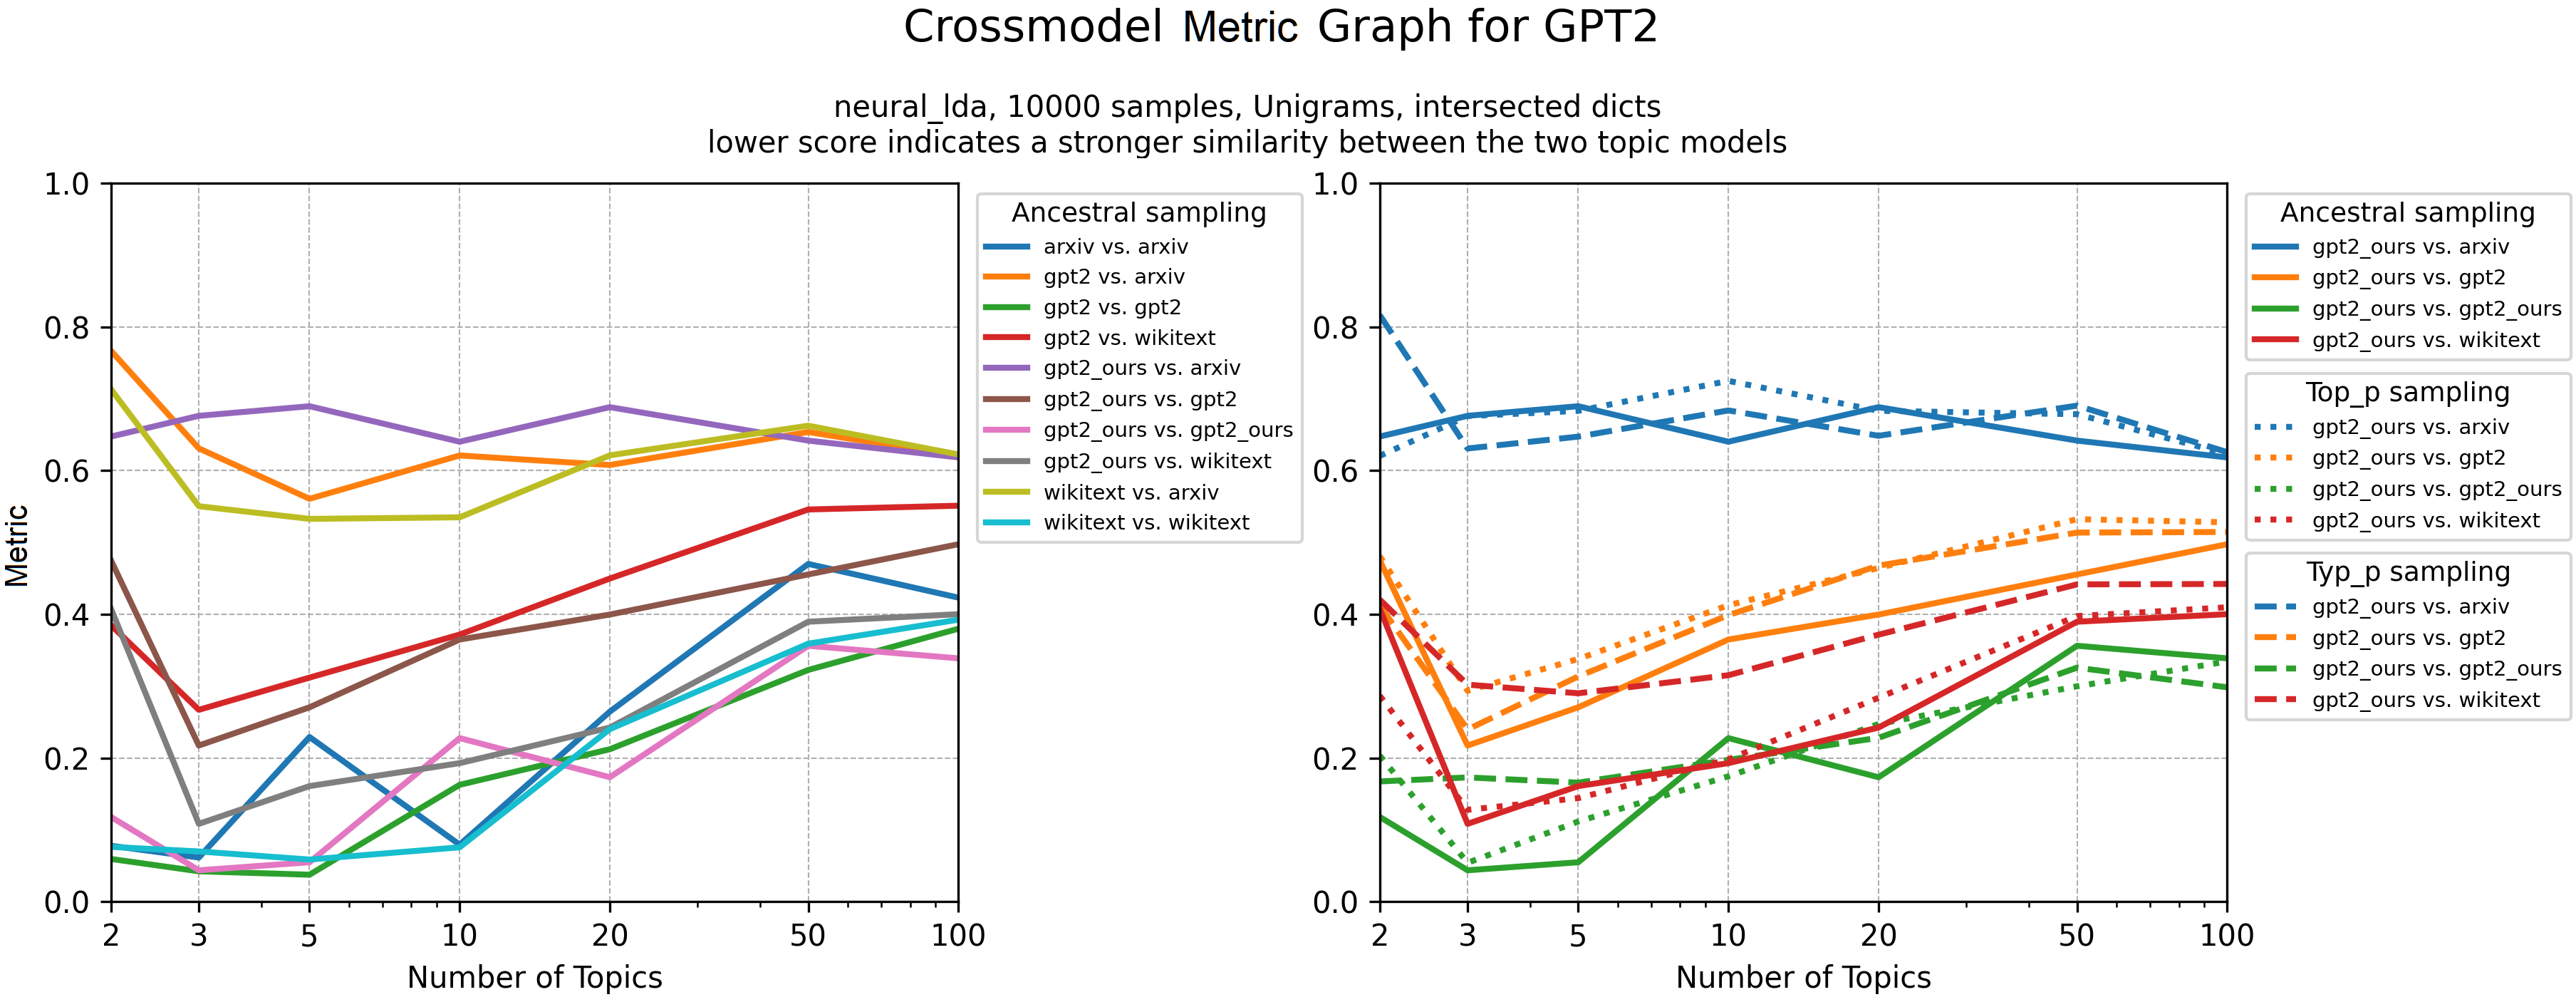
\includegraphics[width=1\textwidth]{figures/Unigrams-10000-crossmodel-tt-gpt2-neural_lda-ab-is}
    \caption{Topic model comparison metric (GPT-2, neural LDA, 10'000 samples).}
    \label{fig:Unigrams-10000-crossmodel-tt-gpt2-neural_lda-ab-is}
\end{figure}

% =======================================
\subsubsection{Transformer-XL and Neural LDA}
In the results for Transformer-XL and topic models created with neural LDA (see \ref{fig:Unigrams-10000-crossmodel-tt-trafo_xl-neural_lda-ab-is} on the left), we find the same tendencies as with the results for GPT-2 topic models created with neural LDA. The \texttt{arxiv} corpus compared to other corpora results in a value above $0.5$ and when comparing topic models from the same corpora, the upper boundary is generally increasing from $0.2$ for a topic size of 2 up to $0.5$ for a topic size of 100. The results of the comparisons between topic models from corpora \texttt{trafo\_xl\_ours} and \texttt{wikitext} fall into the area of similarity, except for 2 topics. There we can see a distinctive difference once again.

Other sampling methods have a rather chaotic impact on some of our results. In fig. \ref{fig:Unigrams-10000-crossmodel-tt-trafo_xl-neural_lda-ab-is} on the right, we can see no impact on the comparison with the topic models from \texttt{arxiv} (the blue lines) but a rather chaotic impact on the comparison of \texttt{trafo\_xl\_ours} with itself (the green lines). The comparison between \texttt{trafo\_xl\_ours} and \texttt{wikitext} (the red lines) shows a kind of smoothing of the metric line when comparing ancestral sampling with Top-P sampling and then with Typical sampling. 
\begin{figure}[H]
    \centering
    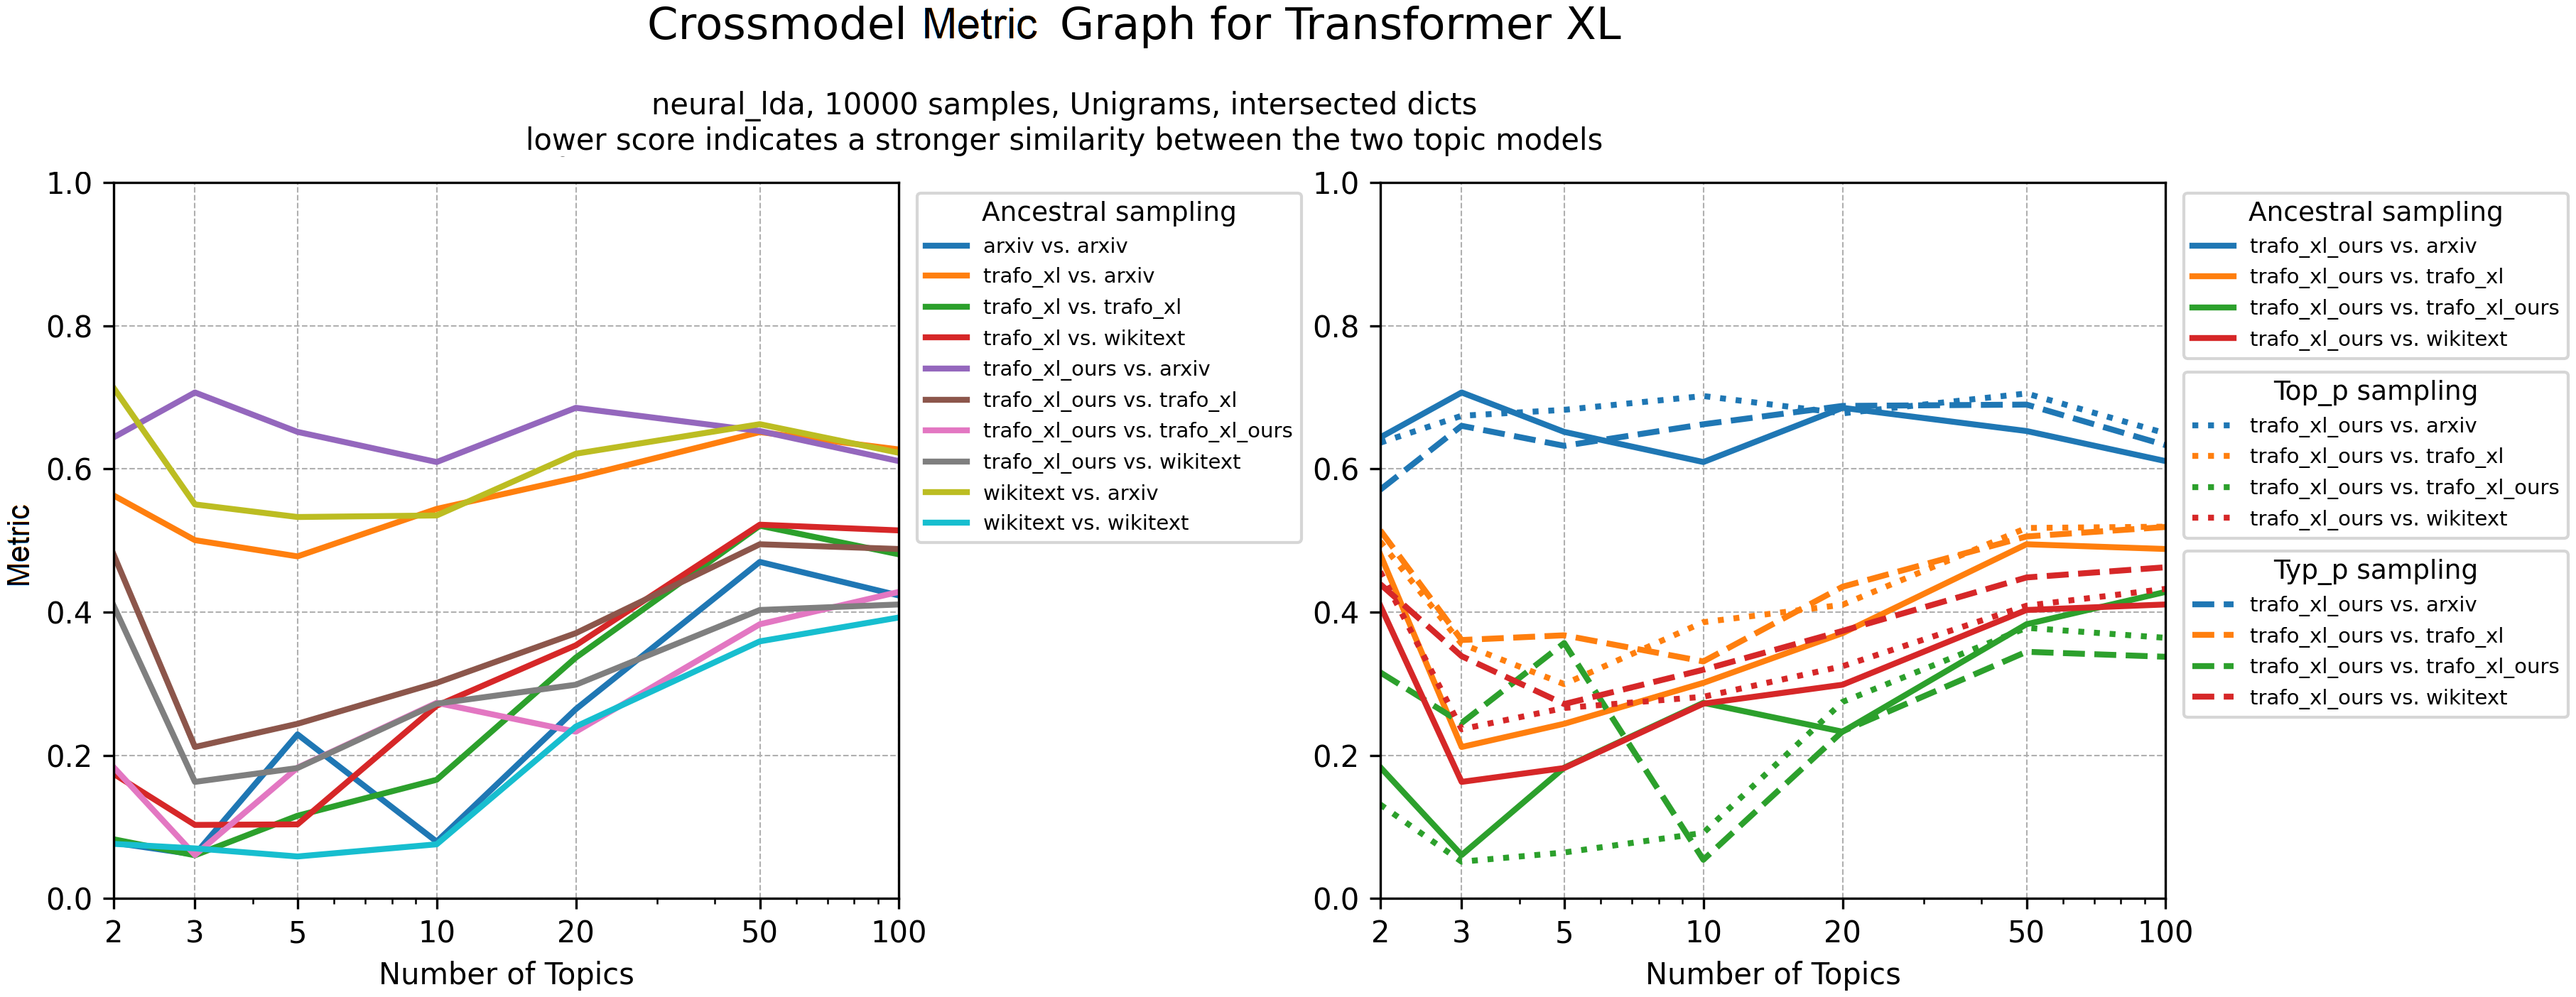
\includegraphics[width=1\textwidth]{figures/Unigrams-10000-crossmodel-tt-trafo_xl-neural_lda-ab-is}
    \caption{Topic model comparison metric (Transformer-XL, neural LDA, 10'000 samples).}
    \label{fig:Unigrams-10000-crossmodel-tt-trafo_xl-neural_lda-ab-is}
\end{figure}

\chapter{Discussion}
In this chapter we are discussing what conclusions we can draw from our results presented in sec. \ref{sec:results} and in which directions future research could go.

% =======================================
\section{Conclusion}
% =======================================
\subsection{The Quality of Our Topic Models}
The results from our measurements regarding the quality of our topic models indicate that the created topic models tend to be stable in their quality when varying the seed and even with slightly changed dictionaries. Furthermore, topic models created with classic LDA tend to have a higher quality than the ones created with neural LDA. Topic models from neural LDA have an interesting inverse peak at 3 topics and tend to produce topic models with nearly the same quality for a topic size of 5 or more when using ancestral sampling.

In the original papers of GPT-2 \cite{gpt-2} and Transformer-XL  \cite{transformer-xl}, the coherence score $C_v$ for their testset is between $0.35$ and $0.60$. Thus, our topic models have a good correlation to human topic-ranking data, especially those with a higher number of topics which can be seen in table \ref{fig:summary}. Regarding different sampling techniques, we see that on average Top-P and even more so Typical sampling clearly improve the quality of topics created by topic models.  
\begin{figure}[H]
    \centering
    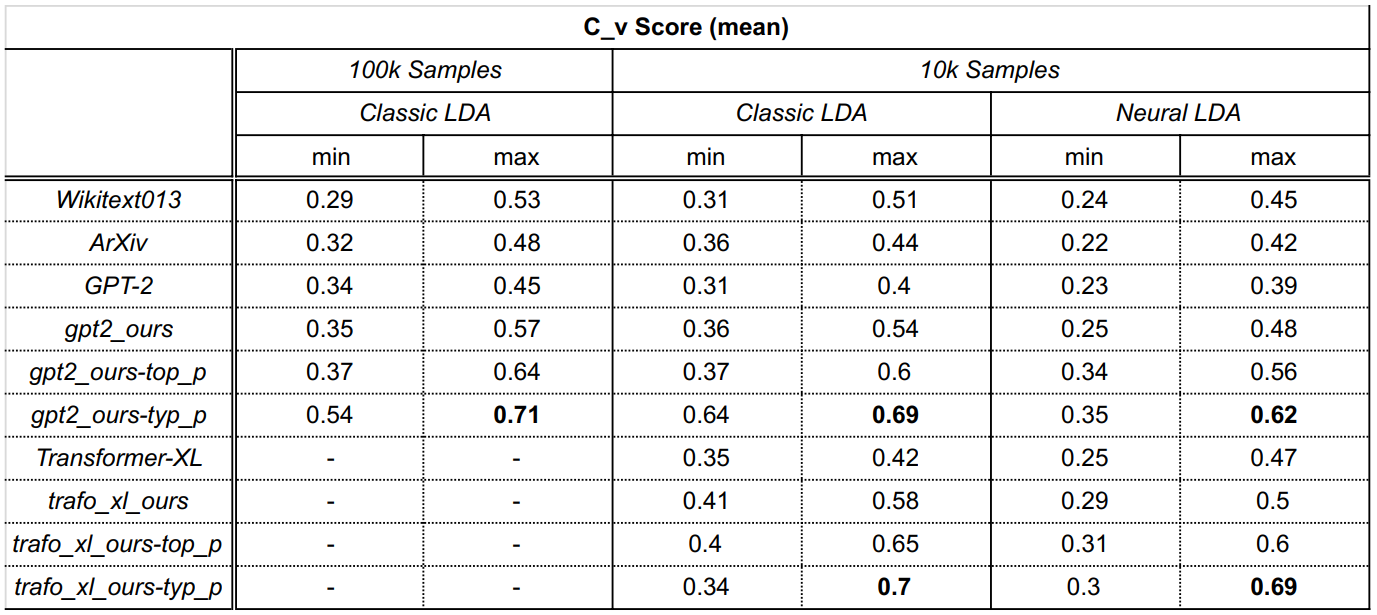
\includegraphics[width=1\textwidth]{figures/Unigrams-cv-var-table-is}
    \caption{$C_v$ topic coherence score table with min and max mean values computed over all topic models.}
\label{fig:summary}
\end{figure}

% =======================================
\subsection{Comparing the Semantic Spaces}
The results from the comparison between topic models with corpora of 100'000 documents clearly show dissimilarities between the sampled corpus and the corpus the GPT-2 model was trained on. With our variance analysis, we can say with a good degree of confidence that these findings are solid for a topic size of 10 or more. In general, we expect the two topic distributions from training dataset and generated dataset to be similar, as the goal of our language model is to learn the language of the corpus it is trained on. This indicates that there is something that skews the model's topic distribution. To find out what is causing this, we have to look at the results from the comparison of topic models with corpora of 10'000 documents. 

First, through our variance analysis for topic models of corpora with 10'000 documents, we have to take a variation of up to $0.1$ for a topic size of 5 or more into account. This makes the interpretation rather vague and we conclude that topic models from corpora with 10'000 documents are not ideal for interpretations. Nonetheless, in our comparison we see that dissimilar topic models result in a value of $0.5$ or higher. This strongly correlates to our findings with corpora of 100'000 documents. For similar topic models, the values tend to be under $0.2$ for a topic size of 10 or lower. For a topic size higher than 10, the area of similar topic models tends to be under $0.4$. This differs from our first findings where the area for similar topic models remains under $0.2$ across all topic sizes. The comparison of the topic models from the sampled corpus and the corpus the GPT-2 model, respectively the Transformer-XL model, was trained on, lies in the area of similarity. This again differs from our first findings where we see a clear discrepancy. We can conclude that if there is a strong inductive bias from the model architecture, we can assume we would see some discrepancies even in topic models from corpora with just 10'000 documents. 

Concerning the differences between the GPT-2 and Transformer-XL results, we expect the topic models created from the original Transformer-XL model to behave similarly to the model we trained ourselves. This is because the original Transformer-XL model was also trained on the Wikitext103 corpus. This assumption is reflected in our results for \texttt{trafo\_xl\_ours} vs. \texttt{trafo\_xl}. It also makes sense that the results from GPT-2 and Transformer-XL did not differ much. Both underlying architectures are based on the decoder model from the Transformer architecture. It backs our proposed approach because we can see similar results with a similar language model architecture. 

As for the differences between the classic LDA and the neural LDA, we come to the same conclusions as with classic LDA. The difference of the learned semantic space and the original one tend to appear similar. There is no clear indication that something skews with the topic distributions. What can clearly be seen in the graphs is that both topic model techniques have the same area of similarity and area of dissimilarity for a corpus size of 10'000 documents. This also backs our proposed approach as the produced results are very similar across different topic modeling techniques.

As for corpora created with different sampling techniques (ancestral, Top-P and Typical sampling), we see that different sampling methods always lead to a skewed topic distribution. By looking at the red lines in all the graphs with all three sampling methods (sec. \ref{sec:comp}, the graphs on the right), we can see that Top-P sampling and even more Typical sampling in general influence the topic distributions. We therefore conclude that the sampling methods Top-P and even more so Typical sampling introduce a generalization to the predicted output which overrules some of the meanings in the semantic spaces. Such an impact is rather unlikely if there is a strong inductive bias in the language model architecture.

% =======================================
\subsection{Summary}
With our new approach to probing language models, we show that by analyzing the differences from various topic distributions, we gain a better understanding of the characteristics of the language learned by today's language models. Furthermore, we are closer than before to being able to identify the isolated impact the inductive bias has on our metric. With this, we show a way to finding out what components of the learning algorithm lead to certain inductive biases. We find discrepancies in the semantic space that are linked to the different methods and parameters we applied but also to the language model algorithm itself. We give a baseline for how to use our method, and build a foundation on which further research can be built. 

% =======================================
\section{Further Work}
After providing the groundwork, our method can be further enhanced and explored in various ways. 

By focusing on the topic model part, the method itself can be extended to work with non-LDA-based topic models \cite{karami2018fuzzy, zhang2022pre}. Additionally, a different approach to tokenization and dictionary creation can lead to more stable and more meaningful topic models which is reflected in the metric. This can help to better identify the differences in the semantic space over corpora of different sizes. We tried incorporating bigrams and trigrams into our topic models but could not to see any notable difference between them. This does not mean they have no influence, just that our implementation did not show any.

By putting the focus on the language model, the method itself can be extended to work with other language model architectures, e.g. encoder based architectures. Additionally, different approaches to train the language model, like changing the loss function and the training parameters, can provide an insight into the influence of architectural properties on the semantic space. All in all, comparing the behaviour of our metric with different language models might tell us what components of the learning algorithm lead to certain inductive biases, which leads in itself to a change in the choice of language model for specific downstream tasks.

Furthermore, by changing the training data for the language models, i.e. using a completely different dataset or an altered version, can give us an insight into how the inductive bias of one language model architecture affects the learning behaviour with different learning data. This might lead to conclusions on how today's language models are trained and how we utilize training data. 

We also suggest to test the stability of our method for a higher corpus size than 10'000 documents, as this will provide answers to how reproducible the results of our metric are and how the language models inductive bias is reflected on different corpus sizes.

If we consider a totally different direction instead of focusing on the inductive bias, we can shift our view to how we can utilize the learned topic distributions from a language model. We could try to influence the probability of a produced string of a language model by combining the learned topic distribution with the intermediate conditional probability over words from a language model. This could help us increase the probability of a string with a certain topic, which is especially interesting when the topic is not very common in the learned language. By analyzing the topics themselves, we could see where the semantic space differs on a word level. Comparing the topic-word distributions with the results or findings from downstream tasks, we could draw conclusions about what specific bias those models exert in those downstream tasks. 

% This displays the bibliography for all cited external documents. All references have to be defined in the file references.bib and can then be cited from within this document.
\bibliographystyle{IEEEtran}
\bibliography{references}

% This creates an appendix chapter, comment if not needed.
%\appendix

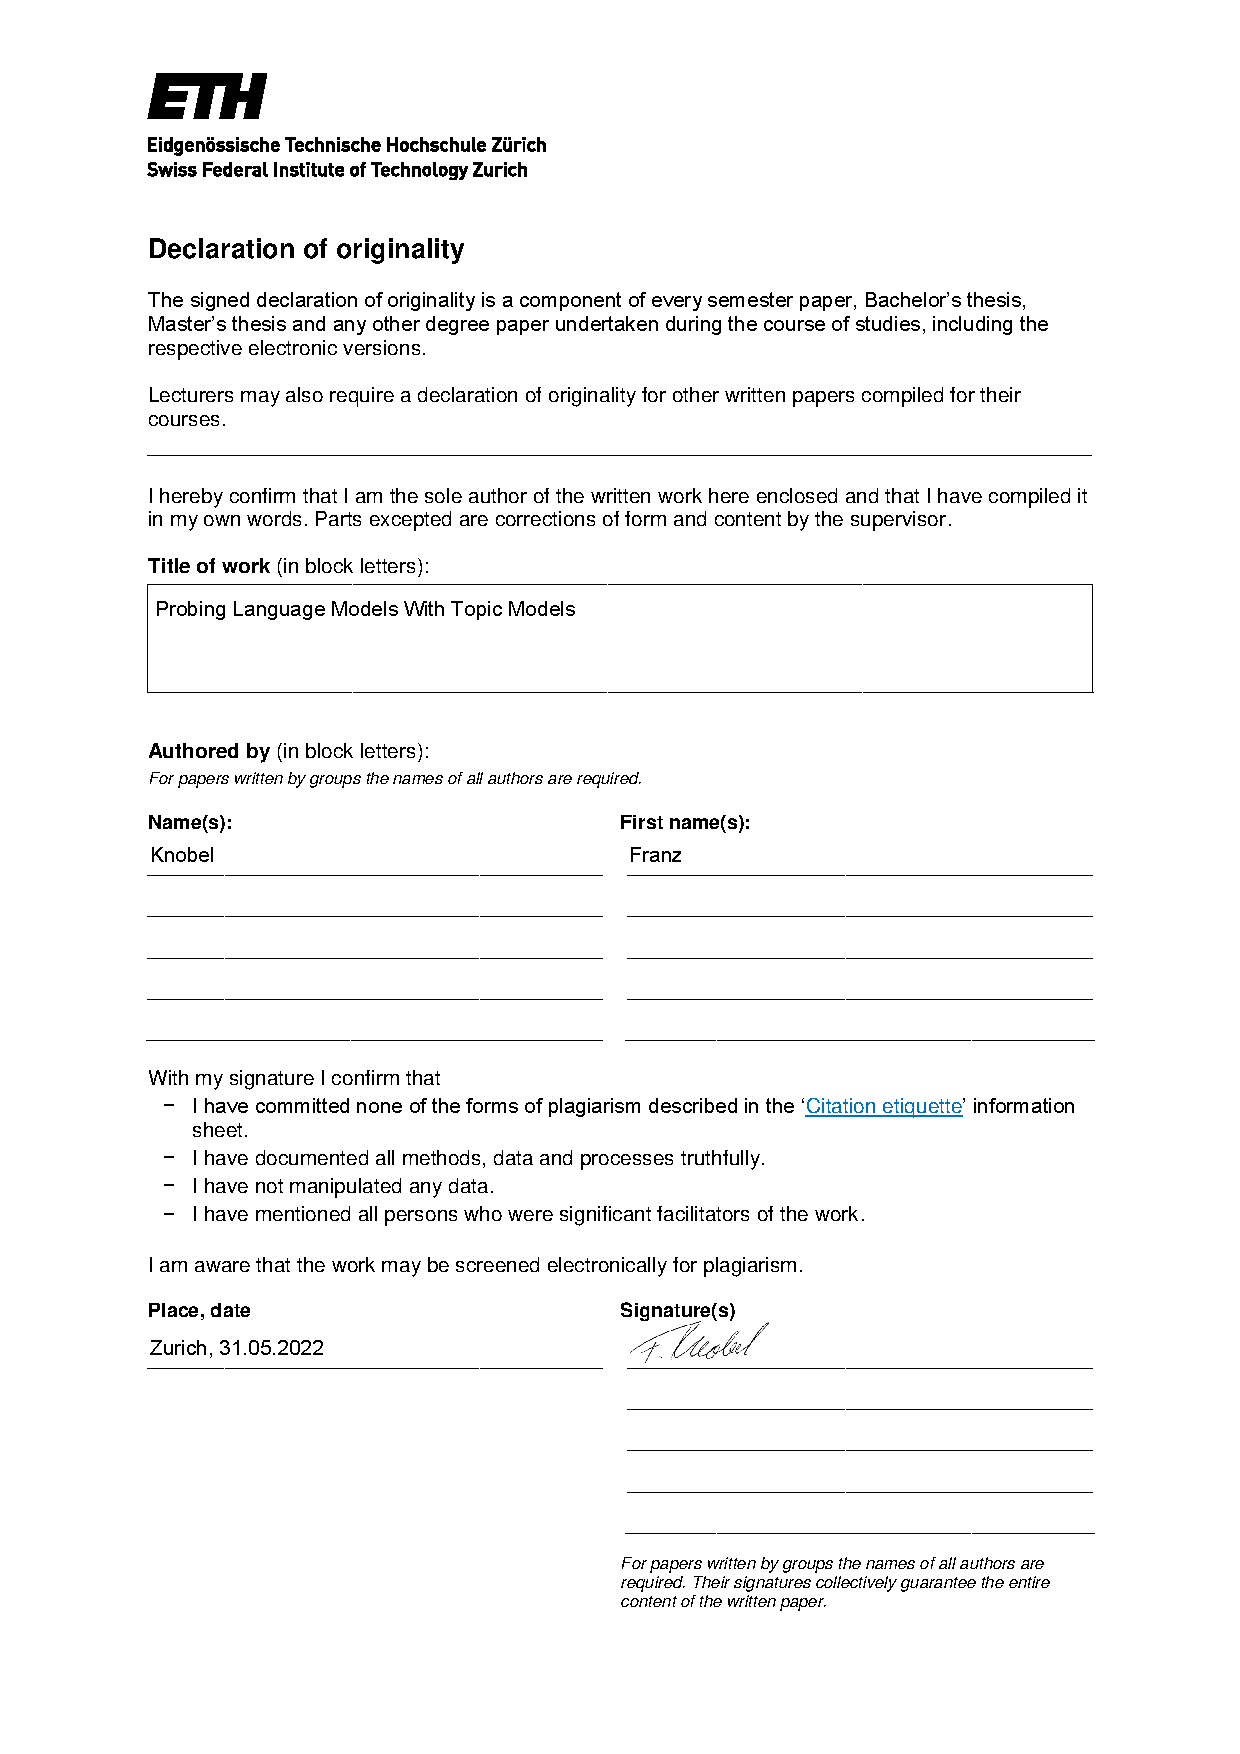
\includepdf[pages={1-},scale=1]{attachments/declaration-originality.pdf}
\end{document}